\documentclass[a4paper, 11pt, openright, twoside]{book}

% Linguistic and standard settings
\usepackage[T1]{fontenc}
\usepackage[utf8]{inputenc}
\usepackage[italian, english]{babel}

\usepackage{comment} 		% Use comment env

\begin{comment}
\usepackage{fancyhdr}
\usepackage{float}
\usepackage{graphicx}
\usepackage{wrapfig}
%------------------------------ colors
\usepackage[usenames,dvipsnames,table]{xcolor} % use colors on table and more
\definecolor{333}{RGB}{51, 51, 51} % define custom color
%------------------------------ source code
\usepackage{listings}
\lstset{
  basicstyle=\footnotesize\sffamily,
  commentstyle=\itshape\color{gray},
  captionpos=b,
  frame=shadowbox,
  language=HTML,
  rulesepcolor=\color{333},
  tabsize=2
}
%------------------------------ define Abstract environment, missing in the 'book' class
\newenvironment{abstract}{\cleardoublepage \null \vfill \begin{center}\bfseries\abstractname \end{center}}{\vfill\null}
\addto\captionsenglish{\renewcommand*\abstractname{Sommario}} % change Abstract title
%------------------------------ active url
\usepackage{url}
\renewcommand{\UrlFont}{\color{black}\small\ttfamily}
\usepackage[colorlinks=true, linkcolor=black, citecolor=black, urlcolor=black]{hyperref} % active ref
%------------------------------ macros
\newcommand{\sectionname}{Section} % define Section ref
\newcommand{\subsectionname}{Sub-section} % define Sub-section ref
\renewcommand*\arraystretch{1.4} % tables padding
\end{comment} 

%%%%%%%%%%%%%%%%%%%%%%%%%%%%%%%%%%%%%%%%%%%%%%%%%%%%%%%%%%%%%%%%%%%%%%%%%%%%% MY STUFF %%%%%%%%%%%%%%%%%%%%%%%%%%%%%%%%%%%%%%%%%%%%%%%%%%%%%%%%%%%%%%%%%%%%%%%%%%%%%

\usepackage{amsmath}
\usepackage{amssymb}
\usepackage{amsthm}
\usepackage{braket} 					% Nice sets
%\usepackage{commath} 					% Nice differential (dx) and derivatives
\usepackage{hyperref} 					% Nice refs
\usepackage[capitalise]{cleveref} 		% Nicer refs
\usepackage{emptypage} 					% Remove headings from blank pages
\usepackage{enumitem} 					% Lists
\usepackage{fancyhdr} 					% Modify page style
\usepackage{float}
\usepackage[a4paper,width=160mm,top=25mm,bottom=25mm,bindingoffset=6mm]{geometry}		% Modify margins
\usepackage{graphicx}					% Insert figures
\usepackage{caption}					% Nice captions
\usepackage{subfig}						% More figures together
\usepackage{mathtools}
\usepackage{nicefrac}					% Nice inline fractions
\usepackage{stmaryrd}
\usepackage{tikz-cd} 					% Diagrams
\usepackage{titlesec}       			% Modify title formats (e.g. remove 'Chapter')
\usepackage{verbatim}
\usepackage[swapnames]{frontespizio}
\usepackage{lipsum} 					% Write garbage

%------------------------------ define Abstract environment, missing in the 'book' class
\newenvironment{abstract}{
	\cleardoublepage \null \vfill 
	\begin{center}
		\bfseries\abstractname
	\end{center}
}
{\vfill\null}
\addto\captionsenglish{\renewcommand*\abstractname{Abstract}} % change Abstract title


%%% Use smaller fonts for didascalie
\captionsetup{font=small, labelfont={sf, bf}} 

%%% Remove `Chapter` from chapters %%%
\titleformat{\chapter}
{\Huge \normalfont \bfseries}{\thechapter}{1em}{}

%%% Page Styles %%%
\pagestyle{fancy}
\fancyhf{}
\fancyhead[LE]{\bfseries \leftmark}
\fancyhead[RO]{\bfseries \rightmark}
\fancyhead[RE, LO]{\bfseries \thepage}

\setlength{\headheight}{13.6pt}

\renewcommand\chaptermark[1]{\markboth{\thechapter.\space#1}{}} 
\renewcommand\sectionmark[1]{\markright{\thesection.\ #1}} 

%%% Use empty pagestyle instead of plain, to remove chapter page numbering %%%
\makeatletter
\let\ps@plain\ps@empty
\makeatother

%%% Colors setup for refs %%%
\hypersetup{    
	colorlinks=false,
	citecolor=Violet,
	linkcolor=Red,
	urlcolor=Blue
}

%%% Bibliography stuff %%

\usepackage[autostyle]{csquotes}
\usepackage[style=numeric, backend=biber, citestyle=numeric]{biblatex}
\addbibresource{Backmatter/bibliography.bib}

\DeclareBibliographyCategory{book}
\DeclareBibliographyCategory{online}

\addtocategory{book}{robert:padic-analysis}
\addtocategory{book}{koblitz:padic-numbers}
\addtocategory{book}{bourbaki:topologie}
\addtocategory{online}{chen:padics}
\addtocategory{online}{michon:padic-arithmetic}
\addtocategory{online}{thorne:teichmuller}
\addtocategory{online}{conrad:algebraic-closure}

\defbibheading{book}{\section*{Books}}
\defbibheading{online}{\section*{Sites}}

%%% abs and norm %%%
\DeclarePairedDelimiter\abs{\lvert}{\rvert}%
\DeclarePairedDelimiter\norm{\lVert}{\rVert}%

% Swap the definition of \abs* and \norm*, so that \abs
% and \norm resizes the size of the brackets, and the 
% starred version does not.
\makeatletter
\let\oldabs\abs
\def\abs{\@ifstar{\oldabs}{\oldabs*}}

\let\oldnorm\norm
\def\norm{\@ifstar{\oldnorm}{\oldnorm*}}
\makeatother

% New math operators
\DeclareMathOperator{\Ima}{Im}			% Write Im of a function in math mode
\DeclareMathOperator{\dist}{ dist }		% Write dist(A, B) between sets
\DeclareMathOperator{\Log}{Log} 		% Iwasawa continuation of log_p
\DeclareMathOperator{\card}{card}		% Cardinality of a set

% New commands
\newcommand{\N}{ \mathbb{N} }
\newcommand{\Nb}{ \mathbf{N} }
\newcommand{\Z}{ \mathbb{Z} }
\newcommand{\Q}{ \mathbb{Q} }
\newcommand{\R}{ \mathbb{R} } 
\newcommand{\C}{ \mathbb{C} }
\newcommand{\F}{ \mathbb{F} }
\newcommand{\E}{ \mathrm{E} } % Artin-Hasse exponential
\newcommand{\Zp}{ \Z_p }
\newcommand{\Qp}{ \Q_p }
\newcommand{\Fp}{ \F_p }
\newcommand{\Cp}{ \C_p }
\newcommand{\padic}{$p$-adic }
\newcommand{\Qpa}{ \Qp^{\textup{alg cl} } }
\newcommand{\Qpu}{ \Qp^{\textup{unram}  } }
\newcommand{\Zpu}{ \Zp^{\textup{unram}  } }
\newcommand{\ord}{ \textrm{ord}_p\, }  %%% \, is a slight space %%%
\newcommand{\pabs}[1]{ \abs{#1}_p }
\newcommand{\ser}[1]{ \llbracket {#1} \rrbracket } % Write quickly formal power series
\newcommand{\newt}[1]{ \mathfrak{N}(#1) } % Write quickly the Newton polygon of f

% Renewed commands
\renewcommand{\phi}{\varphi}
\renewcommand{\epsilon}{\varepsilon}
\renewcommand{\hat}{\widehat}
\renewcommand{\tilde}{\widetilde}

% Theorem styles
\theoremstyle{plain}
\newtheorem{thm}{Theorem}[chapter]
\newtheorem{prop}[thm]{Proposition}
\newtheorem{lemma}[thm]{Lemma}
\newtheorem{corollary}{Corollary}[thm]

\theoremstyle{definition}
\newtheorem{defn}[thm]{Definition}
\newtheorem{example}[thm]{Example}
%%%%%%%%%%%%%%%%%%%%%%%%%%%%%%%%%%%%%%%%%%%%%%%%%%%%%%%%%%%%%%%%%%%%%%%%%% END OF MY STUFF %%%%%%%%%%%%%%%%%%%%%%%%%%%%%%%%%%%%%%%%%%%%%%%%%%%%%%%%%%%%%%%%%%%%%%%%%%%
\begin{document}
	\frontmatter
	%\begin{titlepage} %------------------------------ TITLE PAGE -------------------------------%
	\begin{center}
		\vbox to0pt{\vbox to\textheight{\vfill 
\includegraphics[width=11.5cm]{images/unipd-light} \vfill}\vss}
		
		\hspace{0.5cm}
		\begin{minipage}{.20\textwidth}
			
\includegraphics[height=2.5cm]{images/unipd-bn}
		\end{minipage}
		\begin{minipage}{.90\textwidth}
			\begin{table}[H]
				\begin{tabular}{l}
					\scshape{\Large{\bfseries{Universit\`a degli Studi di Padova}}} \\
					\hline \\
					\scshape{\Large{Dipartimento di Matematica ``Tullio Levi-Civita''}} \\
				\end{tabular}
			\end{table}
		\end{minipage}
		
		\vspace{1cm}
		\emph{\Large{LAUREA TRIENNALE IN MATEMATICA}} \\
		\vspace{1.5cm}
		\scshape{\Large{\bfseries{On p-adic analysis}}} \\
		%\vspace{0.2cm} \linespread{1} \scshape{\large{\bfseries{(subtitle)}}}
	\end{center}
	
	\vfill
	\begin{normalsize}
		\begin{flushleft}
			  \hspace{45pt} \textit{Laureando} \hspace{160pt} \textit{Relatore}\\
			  \vspace{5pt}
			  \hspace{30pt} \large{\textbf{Carlo Buccisano}} \hspace{70pt} \large{\textbf{Prof. Maurizio Cailotto}}\\
			  \vspace{10pt}
			  %\hspace{260pt} \normalsize{\textit{Co-relatore}}\\
			  %\vspace{5pt}
			  %\hspace{240pt} \large{\textbf{nome cognome}}
		\end{flushleft}
	\end{normalsize}
	
	\vfill
	\begin{center}
		\hspace{-0.2cm}
		\line(1, 0){360}
		
		\textsc{Academic Year 2018/2019}
	\end{center}
\end{titlepage}
	\begin{frontespizio}
	\begin{Preambolo*}
		\renewcommand{\frontinstitutionfont}{\fontsize{16}{19}\bfseries}
		\renewcommand{\frontdivisionfont}{\fontsize{14}{18}\scshape}
		\renewcommand{\fronttitlefont}{\fontsize{20}{24}\bfseries}
		\renewcommand{\frontpretitlefont}{\normalfont\fontsize{20}{22}\selectfont}
		\renewcommand{\frontfixednamesfont}{\normalfont\fontsize{14}{16}\rmfamily}
		\renewcommand{\frontnamesfont}{\fontsize{14}{16}\bfseries}
		\renewcommand{\frontsmallfont}{\fontsize{11}{13}\bfseries}
		\renewcommand{\frontfootfont}{\fontsize{14}{16}\bfseries}
	\end{Preambolo*}
	\Universita{Padova}
	\Divisione{Dipartimento di Matematica ``Tullio Levi-Civita''}
	\Corso[Laurea Triennale]{Matematica}
	%\Titoletto{Data ufficiale sessione di laurea: 5 luglio 2019}
	\Titolo{Analytic functions on $p$-adic fields}
	\Candidato[1152337]{Carlo Buccisano}
	\Relatore{Prof. Maurizio Cailotto}
	%\Annoaccademico{2018-2019}
	\Piede{Data sessione di laurea: 5 luglio 2019\\Anno accademico 2018/2019}
	\Logo{images/sigillo_unipd.jpg}
	\Filigrana[height=15cm]{images/unipd-light.png}
	\Margini{1.5cm}{1.5cm}{1.5cm}{1cm}
\end{frontespizio}
	\chapter*{Introduzione}
	Questa tesi si compone di due parti: nella prima (capitoli 1-3) si costruiscono i vari campi $p$-adici per arrivare a $\Cp$, campo completo e algebricamente chiuso, tentando di emulare il procedimento classico che da $(\Q, \abs{\ }_{\infty})$ porta a $\C$. Nella seconda parte (capitoli 4-5), invece, si studiano le funzioni analitiche su $\Cp$, definite come serie di potenze, con particolare attenzione ad alcune funzioni elementari, come l'esponenziale e il logaritmo, e alle differenze che si presentano nel caso $p$-adico rispetto al caso classico. Infine, nel capitolo 5, viene definito il poligono di Newton, potente strumento per capire subito il raggio di convergenza e l'ordine ($p$-adico) degli zeri di una funzione analitica. \newline
	Più specificamente, nel capitolo 1, dopo aver introdotto la definizione di norma e quella di valore assoluto $p$-adico su $\Q$ (e aver mostrato che definisce una norma non-Archimedea), si dimostra il teorema di Ostrowski, che afferma che ogni norma non banale su $\Q$ è equivalente o al valore assoluto classico o a un valore assoluto $p$-adico, per qualche primo $p$. Viene poi provato che $(\Q, \pabs{\ })$ non è completo e viene definito, nel modo classico, il suo completamento $(\Qp, \pabs{\ })$, analogo di $(\R, \abs{\ }_{\infty})$ nel caso classico. Infine, viene provato un teorema di struttura, che afferma che ogni elemento di $\Qp$ può essere scritto come una serie del tipo $\sum_{i=m}^{+\infty} a_ip^i$, con $a_i \in \{0, \dots, p-1\}$ e $m \in \Z$. \newline
	Nel capitolo 2 si arriva di nuovo a costruire $(\Qp, \pabs{\ })$ in un modo, però, totalmente diverso dal primo e più ``algebrico''. Si parte infatti da $\Zp$, insieme contenente tutti gli elementi del tipo $\sum_{i=0}^{+\infty} a_ip^i$ con $a_i \in \{0, \dots, p-1\}$, equipaggiato con le operazioni di somma con riporto e prodotto alla Cauchy (con riporto). Si mostra che esso è un dominio integrale (qui si capisce perché $p$ debba essere primo) e che contiene gli interi (o meglio, che esiste un monomorfismo $\Z \hookrightarrow \Zp$). Dopo un breve excursus su proprietà generiche dei gruppi topologici (dalle quali si ricaverà che $\Zp$ è uno spazio compatto, completo e metrizzabile), viene mostrata un'altra definizione di $\Zp$: come limite proiettivo degli insiemi $\Z/p^n\Z$. Infine si mostra che $\Qp$ è esattamente il campo delle frazioni di $\Zp$ e si introduce il lemma di Hensel, fondamentale strumento per ``rialzare'' le radici di polinomi da $\Z/p^n\Z$ a $\Zp$, quando il polinomio soddisfa opportune ipotesi. \newline
	Nel capitolo 3, dopo un breve excursus su generiche proprietà di spazi ultrametrici, si studiano le estensioni di campi $K/\Qp$ di grado finito e si vede come si può estendere il valore assoluto $p$-adico a tali campi $K$. Vengono poi classificate in base al loro indice di ramificazione e al grado residuo, con particolare attenzione ad estensioni non ramificate e totalmente ramificate. Dopo aver mostrato una versione analoga del criterio di Eisenstein nel caso $p$-adico, viene mostrato che $\Qp$ ammette estensioni di qualunque grado finito, da cui si ricava che la sua chiusura algebrica, $\Qpa$, ha necessariamente grado infinito su $\Qp$. Infine si mostra che $(\Qpa, \pabs{\ })$ non è completo e si considera il suo completamento $\Cp$, che si mostrerà essere anche algebricamente chiuso. Si noti che qui il caso $p$-adico sembra essere più complicato del caso classico: ciò è dovuto al fatto che $\Qpa$ ha grado infinito su $\Qp$ e dunque la completezza si ``perde'', mentre nel caso classico $\C = \R^{\textup{alg cl}}$ ha grado finito (2) su $\R$ e dunque rimane completo. Infine viene dimostrato un teorema di struttura di $\Cp$, che afferma che ogni elemento è prodotto di una potenza frazionaria (radice di un polinomio del tipo $X^a - p^b$, con $a,b \in \Z$), una radice di 1 e un elemento nel disco aperto di raggio 1 centrato in 1. In realtà, come spiegato alla fine del capitolo 3, i due processi (di costruzione di campi completi e algebricamente chiusi) possono essere fatti in modo totalmente analogo: si considera prima $\Q$, poi la sua chiusura algebrica $\Q^{\textup{alg cl}}$ e si completa quest'ultima rispetto a $\abs{\ }_{\infty}$ per ottenere $\C$ e rispetto a $\pabs{\ }$ per ottenere $\Cp$. Il problema di questa costruzione è la notevole difficoltà che si incontra nello studio di $\Q^{\textup{alg cl}}$.\newline
	Nel capitolo 4 viene introdotta la nozione di funzione analitica su $\Cp$, funzione definita come una serie di potenze (dove esssa converge). Viene provato poi che la stessa formula classica per trovare il raggio di convergenza di una serie di potenze vale anche nel caso $p$-adico (sostituendo chiaramente il valore assoluto $p$-adico a quello classico). Viene anche introdotta le definizione di differenziabilità (e stretta differenziabilità) e viene provato che le funzioni analitiche sono differenziabili nel modo standard (termine a termine). Vengono poi definite le funzioni $\exp_p(X)$ e $\log_p(1 + X)$ (usando le serie di MacLaurin note dal caso classico) e viene provato che, a differenza del caso reale, la funzione esponenziale converge solo su un piccolo disco aperto centrato in 0 (di raggio $r_p = p^{-1/(p-1)}$). Le proprietà classiche di esponenziale e logaritmo, però, si conservano anche nel caso $p$-adico e, restringendo in maniera appropriata dominio e codominio, si mostra che esponenziale e logaritmo sono funzioni l'una inversa dell'altra. Infine si introducono due nuove funzioni: il logaritmo di Iwasawa e l'esponenziale di Artin-Hasse. La prima è una funzione localmente analitica, definita su tutto $\Cp$, che estende il logaritmo precedentemente definito e ha derivata $x \mapsto 1/x$. L'esponenziale di Artin-Hasse, invece, è ricavato togliendo i termini ``problematici'' dall'esponenziale, ottenendo così una più estesa regione di convergenza (più specificamente viene prima mostrato un modo per scrivere $\exp_p(X)$ come prodotto infinito di serie di potenze e viene poi notato che sono solo alcuni di questi termini a imporre una minore regione di convergenza: togliendoli si ottiene l'esponenziale di Artin-Hasse). Nonostante il nome che potrebbe trarre in inganno, esso non è un'estensione dell'esponenziale: infatti vale $\E_p(X) = \exp_p\left(X + \tfrac{X^p}{p} + \tfrac{X^{p^2}}{p^2} + \dots\right)$. \newline
	Nell'ultimo capitolo viene introdotta la definizione di poligono di Newton prima per i polinomi e poi per le serie di potenze. Viene poi presentato l'importante teorema che lega gli zeri di un polinomio al suo poligono di Newton: infatti per ogni segmento di pendenza $\lambda$ e di lunghezza $M$ (qui per lunghezza si intende quella della proiezione sull'asse orizzontale) vi sono esattamente $M$ zeri, contati con molteplicità, di ordine $p$-adico $-\lambda$ e tutti gli zeri sono ottenuti in questo modo. Dopo aver mostrato che il raggio di convergenza di una serie è esattamente il $\sup$ delle pendenze del suo poligono di Newton si mostrano dei lemmi tecnici per arrivare a dimostrare il teorema di separazione di Weierstrass. Esso ha, tra i suoi corollari, la generalizzazione alle serie di potenze del teorema precedentemente enunciato solo per i polinomi, ossia per ogni segmento di lunghezza $N < +\infty$ e di pendenza $\lambda$ si hanno $N$ zeri della serie di ordine $p$-adico $-\lambda$. L'ultimo risultato mostrato è che ogni serie di potenze $f(X) \in 1 + X\Cp\ser{X}$ convergente su tutto $\Cp$ ha un insieme di zeri numerabile, sia $(r_n)_{n \in \N}$, e vale $f(X) = \prod_{n \in \N} \left(1 - \tfrac{X}{r_n}\right)$. Possiamo pensare a tale risultato come ad una generalizzazione del teorema fondamentale dell'algebra (esiste una versione di tale teorema anche su $\C$, ma si ottiene un prodotto con fattori più complicati). Tra le conseguenze di quest'ultimo vi è ad esempio il fatto che non può esistere, su $\Cp$, un esponenziale come nel caso classico, ossia ovunque convergente e mai nullo: infatti qualunque serie del genere deve essere una costante.
	
	%\cleardoublepage % make left page blank
	\begin{comment}
		\thispagestyle{empty} %------------------------------ DEDICA
		
		\null
		\vspace{2cm}
		\begin{flushright}
		A ...
		\end{flushright}
		\vfill
		
		\begin{quote}
		  Quote
		
		  \textit{Author}
		\end{quote}
		\vfill
		\null
	\end{comment}
	
	
	\begingroup %------------------------------ CONTENTS
	  \makeatletter
	  \let\ps@plain\ps@empty
	  \makeatother
	  \tableofcontents
	  \clearpage
	\endgroup
	
	\mainmatter
	\setcounter{chapter}{0}
	%part{Setting up the p-adic environment}
	\chapter{Analytic Approach}
	\section{Basic concepts}
		Here we'll define some basic concepts about norms and metrics. 
		\begin{defn}
			Let $X$ be a non-empty set, a function $d\colon  X \times X \to \R_{\geq 0}$ is a \textit{metric} if, for every $x, y, z \in X$, we have:
			\begin{enumerate}
				\item $d(x, y) = 0 \iff x = y$;
				\item $d(x, y) = d(y, x)$;
				\item $d(x, y) \leq d(x, z) + d(z, y)$.
			\end{enumerate}
		\end{defn}
		\begin{defn}
			\label{defn:field-norm}
			Let $F$ be a field, a function $\norm{\ }\colon F \to \R_{\geq 0}$ is a \textit{field norm}\footnote{Although usually the term ``field norm'' has a different definition in field theory, we choose to use this terminology, to distinguish between norms on fields and norms on vectorial spaces.}(or an \textit{absolute value}) if, for every $x, y \in F$, we have:
			\begin{enumerate}
				\item $\norm{x} = 0 \iff x = 0$;
				\item $\norm{x \cdot y} = \norm{x} \cdot \norm{y}$;
				\item $\norm{x + y} \leq \norm{x} + \norm{y}$.
			\end{enumerate}
		\end{defn}
		\begin{defn}
			Let $V$ be a vector space over the field $F$, which has its norm $\norm{\ }_F$. A function $\norm{\ }\colon V \to \R_{\geq 0}$ is a \textit{norm} if, for every $v, w \in V, \alpha \in F$, we have:
			\begin{enumerate}
				\item $\norm{v} = 0 \iff v = 0$;
				\item $\norm{\alpha \cdot v} = \norm{\alpha}_F \cdot \norm{v}$;
				\item $\norm{v + w} \leq \norm{v} + \norm{w}$.
			\end{enumerate}
		\end{defn}
		Beginning from a (field) norm $\norm{\ }$ there's a natural metric defined as $d(x, y) = \norm{x - y}$.
	\section{Metrics on $\Q$}
		The metric we normally equip $\Q$ with is the euclidean one, which comes from the usual absolute value $\abs{\ }$ (denoted also by $\abs{\ }_\infty$). 
		\begin{defn}
			Let $p$ a fixed prime. We can define a function $\ord\colon \Z \to \N \cup \{+\infty \}$ as follows: 
			\begin{equation*}
				\ord a := 
				\begin{cases*}
					+\infty, & \text{if $a = 0$;} \\
					n_a, & \text{otherwise;}
				\end{cases*} 
			\end{equation*}
			where $n_a \in \N$ is such that $p^{n_a} | a$ and $p^{n_a + 1} \nmid a$. It's easy to prove that $\ord ab = \ord a + \ord b$ (using the usual convention $\infty + n = n + \infty =+\infty$).
		\end{defn}
		We can extend this function to $\Q$:
		\begin{equation*}
			\ord \left( \frac{a}{b} \right) := 
			\begin{cases*}
				+\infty, & \text{if $\frac{a}{b} = 0$;} \\
				\ord a - \ord b, & \text{otherwise;}
			\end{cases*}.
		\end{equation*}
		This is of course well defined: $\ord \left( \tfrac{ac}{bc} \right) = \ord ac - \ord bc = \ord a - \ord b = \ord \left( \tfrac{a}{b} \right)$. 
		\begin{prop}
	 		$\emph{ord}_p\colon  \Q \to \Z \cup \{+\infty\}$ is a discrete valuation.
		\end{prop}
		\begin{proof}
			We have to prove the following properties:
			\begin{itemize}
				\item $\ord x = +\infty \iff x = 0$;
				\item $\ord xy = \ord x + \ord y$;
				\item $\ord (x + y) \geq \min \{\ord x, \ord y \}$.
			\end{itemize}
			The first two properties are quite easy, to see why the third one is true it's sufficient to write 
			\[
				x = \frac{a}{b} = p ^ {\ord x} \cdot \frac{a'}{b'}, \qquad y = \frac{c}{d} = p^{\ord y} \cdot \frac{c'}{d'}
			\]
			with $a', b', c', d'$ coprime with $p$. Then
			\begin{equation*}
				x + y = p^{\min \{\ord x,\,\ord y \}} \cdot q \qquad (q \in \Q).
			\end{equation*}
			Applying property $2.$ from \cref{defn:field-norm} we obtain
			\begin{gather*} 
				\ord(x + y) = \ord \left(p^{\min \{\ord x,\,\ord y \}} \cdot q\right) \geq \min \{\ord x, \ord y \}.\qedhere
			\end{gather*}
		\end{proof}
		
		Using these functions we can define a field norm $\pabs{\ }\colon \Q \to \Q$ as follows:
		\begin{equation*}
			\pabs{x} = 
			\begin{cases*}
				p ^ {-\ord x}, & if $x \neq 0$; \\
				0, & otherwise;
			\end{cases*}.
		\end{equation*}
		\begin{prop}
			\label{prop:padic-nonarchimedean}
			$\pabs{\ }$ is a field norm on $\Q$.
		\end{prop}
		\begin{proof}
			Property $1.$ is obvious. \newline
			To prove $2.$, given $x, y \in \Q^{\times}$ we know that $\ord xy = \ord x + \ord y$ so 
			\begin{gather*}
				\pabs{xy} = p^{- \ord xy} = p^{-\ord x - \ord y} = p^{-\ord x} \cdot p^{-\ord y} = \pabs{x} \cdot \pabs{y}.
			\end{gather*}
			To prove $3.$ let $x, y \in \Q^{\times}$; $\ord(x + y) \geq \min \{\ord x, \ord y\}$ so
			\begin{gather*}
				\pabs{x + y} = p^{-\ord(x + y)} \leq p^{- \min \{\ord x,\, \ord y \} } = p ^ {\max \{-\ord x,\,-\ord y\} } \\
				= \max \left\{p ^ {-\ord x}, p^{-\ord y} \right\} = \max \left\{\pabs{x}, \pabs{y} \right\} \leq \pabs{x} + \pabs{y}.
			\end{gather*}
			We actually proved a stronger inequality than $3.$, which is one of the key ingredients of \padic analysis.
		\end{proof}
		\begin{defn}
			A norm on $X$ is called \textit{non-Archimedean} if $\norm{x + y} \leq \max \left\{\norm{x}, \norm{y} \right\}$ holds for every $x, y \in X$. 
		\end{defn}
		If $\norm{\ }$ is a non-Archimedean norm on $X$, it's immediate to see that
		\begin{gather*}
			\norm{n\cdot x} \leq \norm{x} \text{ for every $n \in \N, x \in X$ }
		\end{gather*}
		which explains the name. We have already proved that $\pabs{\ }$ is a non-Archimedean norm on $\Q$ in \cref{prop:padic-nonarchimedean}.
		\begin{prop}
			If $\norm{\ }$ is a non-Archimedean norm on $X$ then
			\[
				\norm{x} \neq \norm{y} \implies \norm{x + y} = \max \left\{\norm{x}, \norm{y} \right\}.
			\] 
		\end{prop}
		\begin{proof}
			We can assume that $\norm{x} < \norm{y}$. Then
			\begin{gather*}
				\norm{y} = \norm{(x + y) - x} \leq \max \left\{\norm{x+y}, \norm{x}\right\} \leq \norm{y}
			\end{gather*}
			but since $\norm{x} < \norm{y}$ we must have $\norm{x+y} = \norm{y}$.
		\end{proof}
		\begin{defn}
			If $(X, d)$ is a metric space, a sequence $(a_n)_{n \in \N}$ is a \textit{Cauchy sequence} if $\forall \varepsilon > 0$ $\exists n_0 \in \N$ such that $n, m > n_0 \implies d(a_n, a_m) < \varepsilon$.
		\end{defn}
		\begin{defn}
			Two metrics $d_1, d_2$ on $X$ are \textit{equivalent} if every Cauchy sequence for $d_1$ is Cauchy for $d_2$ and vice-versa. Two norms are equivalent if they induce equivalent metrics.
		\end{defn}
		Now we present a technical lemma we're going to need.
		\begin{lemma}
			\label{lemma:equivalent-norm}
			If $\alpha \in (0, 1]$ the function on $\Q$ defined by $x \mapsto \abs{x}^\alpha$ is a norm equivalent to $\abs{\ }_\infty$.
		\end{lemma}
		\begin{proof}
			First of all we show $\abs{\ }^\alpha$ is actually a norm; property $1.$ and $2.$ are easily verified. To prove $3.$ we have to show that $\abs{x + y}^\alpha \leq \abs{x}^\alpha + \abs{y}^\alpha$ for every $x, y \in \Q^{\times}$. We can assume $0 < x < y$ and, dividing both sides by $\abs{y}^\alpha$, we just need to prove $(1 + t)^\alpha \leq 1 + t^\alpha$ for $t \in [0, 1]$. This easily follows studying the first derivative of $[0, 1] \ni t \mapsto 1 + t^\alpha - (1 + t)^\alpha$ (always non negative if $0 \leq \alpha \leq 1$).\newline
			The equivalence of the two norms is easy to see if we use the above definition: let $(a_n)_n$ be Cauchy for $\abs{\ }$; fixed $\varepsilon > 0$ we can find $n_0 \in \N$ such that $n, m > n_0 \implies \abs{a_n - a_m} < \varepsilon ^ \frac{1}{\alpha}$ i.e. $\abs{a_n - a_m}^\alpha < \varepsilon$ $\forall n, m > n_0$ so $(a_n)_n$ is also Cauchy for $\abs{\ }^\alpha$ (and vice-versa).
		\end{proof}
		Generalizing a little bit the previous lemma we can prove that if $\norm{\ }_1$ and $\norm{\ }_2$ are two field norms on $F$ which satisfy $\norm{x}_1 = \norm{x}_2^\alpha$ $\forall x \in F$ for a fixed $\alpha > 0$ then they're equivalent. For example, instead of defining $\pabs{\ }$ using $p ^ {- \ord a}$, we could have used $\rho \in (0, 1)$ in place of $1/p$ and we would have obtained an equivalent norm because $p^ {-\ord a} = \left(\rho ^ {\ord a}\right)^{-\log_\rho p}$.
		\begin{defn}
			The norm $\norm{\ }$ such that $\norm{x} = 1 - \delta_0^x$ is called \textit{trivial}.
		\end{defn}
		Finally we can prove the main theorem of this section.
		\begin{thm}[Ostrowski]
			Every non-trivial norm $\norm{\ }$ on $\Q$ is equivalent to $\pabs{\ }$ for some prime $p \in \N$ or for $p = \infty$.
		\end{thm}
		\begin{proof}
			We distinguish two cases.\newline
			\textit{Case} (1). There exists a positive integer $n$ such that $\norm{n} > 1$. Let $n_0$ be the minimum among those (for every field norm $\norm{\pm 1} = 1$ so $n_0 > 1$). Since $\norm{n_0} > 1$ there exists $\alpha = \log_{n_0}\norm{n_0} > 0$ such that $\norm{n_0} = n_0^\alpha$. Now if $n \in \N^{\times}$ then, using base $n_0$, we can write
			\begin{equation*}
				n = a_0 + a_1n + \dots + a_sn_0^s, \qquad a_i \in \{0, 1, \dots, n_0-1\}, a_s \neq 0.
			\end{equation*}
			Then, since norms are subadditive and multiplicative
			\begin{gather*}
				\norm{n} \leq \norm{a_0} + \norm{a_1n_0} + \dots + \norm{a_sn_0^s} = \\
				= \norm{a_0} + \norm{a_1}n_0^\alpha + \dots + \norm{a_s}n_0^{s\alpha}.
			\end{gather*}
			Being $n_0$ the minimum positive integer with $\norm{n_0} > 1$ we have $\norm{a_i} \leq 1$ so
			\begin{gather*}
				\norm{n} \leq 1 + n_0^\alpha + \dots + n_0^{s\alpha} \leq n_0^{s\alpha}(1 + n_0^{-\alpha} + \dots + n_0^{-s\alpha}) \leq 
	 			n^\alpha \left[\sum_{i=0}^{\infty} n_0^{-i\alpha} \right].
			\end{gather*}
			The last inequality is true because $n \geq n_0^s$. The series at the right side is a geometric one which converges to a certain $C < +\infty$ (since $0 < \frac{1}{n_0} < 1$). Now we have obtained
			\begin{equation*}
				\norm{n} \leq Cn^\alpha.
			\end{equation*}
			Using $n^N$, for some large $N \in \N$, in place of $N$ in the last inequality, and then extracting $N$th roots, leads us to
			\begin{equation*}
				\norm{n} \leq \sqrt[N]{C}n^\alpha.
			\end{equation*}
			Letting $N \to +\infty$ we get $\norm{n} \leq n^\alpha$ (obviously this is valid for every $n \in \N$). To get the other verse of the inequality, using $n$ written as above, we have $n_0^{s+1} > n \geq n_0^s$. Using reverse triangular inequality and the one we obtained above, we get
			\begin{equation*}
				\norm{n} \geq \norm{n_0^{s+1}} - \norm{n_0^{s+1} - n} \geq n_0^{(s+1)\alpha} - \left(n_0^{s+1} - n\right)^\alpha.
			\end{equation*}
			Since $n > n_0^s$
			\begin{equation*}
				\norm{n} \geq n_0^{(s+1)\alpha} - \left(n_0^{s+1} - n_0^s\right)^\alpha = n_0^{(s+1)\alpha} \left[1 - \left(1 - \frac{1}{n_0} \right) ^ \alpha \right] \geq C'n^\alpha
			\end{equation*}
			with $C' := \left[1 - \left(1 - \frac{1}{n_0} \right) ^ \alpha \right]$ that doesn't depend on $n$. As before, using $n^N$ and taking $N$th roots and letting $N \to +\infty$ gives $\norm{n} \geq n^\alpha$.
			So we proved that $\norm{n} = n^\alpha$ for every $n \in \N$. Using property $2.$ of norms and $\norm{-1} = 1$ we get $\norm{q} = \abs{q}^\alpha$ for every $q \in \Q$. Now, using \cref{lemma:equivalent-norm}, we conclude that $\norm{\ }$ is equivalent to $\abs{\ }_\infty$.\newline
			\textit{Case} (2). For every $n \in \N$, $\norm{n} \leq 1$. Since $\norm{\ }$ is non-trivial by hypothesis we can find the minimum $\N \ni n_0 > 1$ such that $\norm{n_0} < 1$. Easily $n_0$ is a prime number: if not, $n_0 = a \cdot b$ with $1 < a,b < n_0$ and $1 > \norm{n_0} = \norm{ab} = \norm{a}\norm{b}$ so at least one from $\norm{a}$ and $\norm{b}$ must be strictly less than $1$, absurd because $a, b < n_0$ and $n_0$ is the minimum positive integer with this property. \newline
			Let $p = n_0$ and we claim that if $q$ is a different prime from $p$ $\norm{q} = 1$. If this is not true then $\norm{q} < 1$ and we can find some large $N \in \N$ such that $\norm{p^N}, \norm{q^N} < 1/2$. Since $p^N$ and $q^N$ are coprime, from Bézout identity there are $n, m \in \Z$ such that $np^N + mq^N = 1$, but this leads to a contradiction:
			\begin{equation*}
				1 = \norm{1} = \norm{np^N + mq^N} \leq \norm{n}\norm{p^N} + \norm{m}\norm{q^N} \leq \norm{p^N} + \norm{q^N} < \frac{1}{2} + \frac{1}{2} < 1.
			\end{equation*}
			Now, given $n \in N$ we can factorize it in a unique way into prime divisors $n = p_1^{b_1} \cdots p_r^{b_r}$. At most one from the $p_i$-s is equal to $p$ so if, wlog, $p_1 = p$ then $b_1 = \ord n$ and $\norm{p_i} = 1$ if $i>1$ so
			\begin{equation*}
				\norm{n} = \norm{p_1^{b_1} \cdot \dots \cdot p_r^{b_r}} = \norm{p_1}^{b_1}\cdot \dots \cdot \norm{p_r}^{b_r} = \norm{p}^{\ord n}.
			\end{equation*}
			Letting $\rho := \norm{p} \in (0, 1)$ we obtain $\norm{a} = \rho ^ {\ord a}$ for $a \in \N^{\times}$. Using property $2.$ of norms we can show this holds also if $a \in \Q^{\times}$. We conclude that $\norm{\ }$ is equivalent to $\pabs{\ }$, using the general version of \cref{lemma:equivalent-norm}.
		\end{proof}
		The standard topology of $\Q$, induced by the euclidean metric, is very different from the \padic topology, induced by the \padic ultrametric. With the former, $\Z \subset \Q$ is a discrete set while, in \padic environment, $\Z$ isn't discrete: $0$ is an accumulation point, $\lim_{n \to +\infty}p^n = 0$. There are also some interesting algebraic properties, which we haven't in the standard topology, for example the one described in the following lemma.
		\begin{lemma}
			For every $r > 0$ the set $B_{<r}(0) \cap \Z = \{x \in \Z \mid \pabs{x} < r\}$ is an ideal of the ring $\Z$, in the \padic topology.
		\end{lemma}
		\begin{proof}
			It's clear that we can only consider the case $r = p^k$ with $k \in \Z$. If $k \geq 0$ the property is trivial since $\Z \subseteq B_{\leq 1}(0) = \{x \in \Q \mid \pabs{x} \leq 1 \}$. Let's consider $x, y \in \Z \cap B_{< p^k}(0)$, i.e. $\pabs{x}, \pabs{y} < p^k$. We must show that $\pabs{x - y} < p^k$ and that for every $z \in \Z$ we have $z \cdot x \in B_{<p^k}(0) \cap \Z$. For the first property we have
			\begin{gather*}
				\pabs{x - y} \leq \max \left\{\pabs{x}, \pabs{-y} \right\} = \max \left\{\pabs{x}, \pabs{y} \right\} < p^k
			\end{gather*}
			and for the second one, recalling that $\Z \ni z \implies \pabs{z} \leq 1$, we have
			\begin{gather*}
				\pabs{z \cdot x} = \pabs{z} \cdot \pabs{x} \leq \pabs{x} < p^k. \qedhere
			\end{gather*}
		\end{proof}
	
		These non-Archimedean norms $\pabs{\ }$ have some very strange properties, far from our intuition (which is based on euclidean norms). We'll explore them in detail in \cref{section:ultrametrics}.
	\section{Construction of $\Qp$}
		\label{section:construction-Qp}
		\begin{defn}
			A metric space $(X, d)$ is \textit{complete} if every Cauchy sequence in $X$ converges to some element in $X$.
		\end{defn}
		\begin{defn}
			If $(X, d)$ is a metric space, $(\overline{X}, \overline{d})$ is its completion if it is a complete metric space which contains $X$ as a dense subspace and satisfies this universal property: if $Y$ is a complete metric space and $f\colon X \to Y$ is uniformly continuous then there exists a unique $f'\colon \overline{X} \to Y$ such that $f'$ is uniformly continuous and $f'|_X = f$.
		\end{defn}
		It's clear from the definition that the completion of a space is unique up to isometry.
		\begin{prop}
			\label{prop:Q-not-complete}
			$(\Q, \pabs{\ })$ is not complete.
		\end{prop}
		\begin{proof}
			This proof will heavily rely on the definition of $\Zp$ proposed in \cref{section:Zp}, and on Hensel's lemma (\cref{thm:hensel-lemma}). Obviously we don't need any result depending on this statement to  build $\Zp$ and prove the Hensel's lemma (in other words: this proof does not create any logical loop).\newline
	 		We have to show that there exists a Cauchy sequence in $(\Q, \pabs{\ })$ which has no limit in $\Q$. To do this, we'll use a polynomial $P(X) \in \Z[X] \subset \Zp[X]$ which has no roots in $\Q$ but admits a root in $\Z/p\Z$. We'll then use Hensel's lemma to obtain $\xi \in \Zp$ such that $P(\xi) = 0$. We'll then have a Cauchy sequence in $\Z \subset \Q$ (we can consider truncated sums of $\xi$) which converges to $\xi \notin \Q$. Let's distinguish four cases.
	 		\begin{itemize}
	 			\item $p = 2$: \newline
	 				  Let's consider the polynomial $P(X) = X^3 - 7 \in \Z[X]$: obviously there are no rational roots of $P$ but $x_0 = 1$ is such that $P(x_0) \equiv 0 \mod 2$. We immediately see that $P'(X) = 3X^2$ so $2 \nmid 3 = P'(1)$ and, applying Hensel's lemma, we infer there is a unique $\xi \in \Z_2$ such that $P(\xi) = 0$. 
	 			\item $p = 3$: \newline
		 			  Let's consider the polynomial $P(X) = X^2 - 7 \in \Z[X]$: obviously there are no rational roots of $P$ but $x_0 = 1$ is such that $P(x_0) \equiv 0 \mod 3$. We immediately see that $P'(1) = 2 \not\equiv 0 \mod 3$ and, applying Hensel's lemma, we infer there is a unique $\xi \in \Z_3$ such that $P(\xi) = 0$. 
	 			\item $p \equiv 1 \mod 4$: \newline
	 				  Let's consider the polynomial $P(X) = X^2 - (p+1) \in \Z[X]$. We observe that $P$ has no rational roots; writing $p+1 = 4k + 2$ we immediately see that $p+1$ is not a perfect square, because $2 \mid p+1$ but $4 \nmid p+1$. Clearly, $p+1$ can't either be a square of some rational number: if it were, then we would have
	 				  \[
	 				      p+1 = \left( \frac{a}{b} \right) ^2 \implies b^2\cdot (p+1) = a^2
	 				  \]
	 				  which is an absurd, since $p+1$ is not a perfect square. So $P$ has no roots in $\Q$, but we easily see that $P(1) \equiv 0 \mod p$ and $P'(1) = 2 \not\equiv 0 \mod p$. Applying Hensel's lemma we find $\xi \in \Zp$ such that $P(\xi) = 0$.
	 			\item $p \equiv 3 \mod 4$: \newline
	 				  Let's consider $\left(\frac{p-1}{2}\right)^2 \equiv 4^{-1} \mod p$ and let $t \in \{0, \dots, p-1\}$ such that $4t \equiv 1 \mod p$. Obviously $0 \neq t$ is a quadratic residue in $\Z/p\Z$; we claim that $\sqrt{t} \notin \Q$. We just need to show that $t$ is not a perfect square (then we can use the same reasoning of the previous point). First of all, with a little abuse of notation, we observe that 
	 				  \[
	 				  	  \Fp^2 = \Set{ x^2 | 0 \leq x \leq \frac{p-1}{2}, x \in \N}.
	 				  \]
	 				  Since the only perfect squares less than $p$ are exactly $\Set{x^2 | 0 \leq x \leq \lfloor{\sqrt{p}}\rfloor, x \in \N}$ and $\frac{p-1}{2} \geq \sqrt{p}$ for $p \geq 7$, we infer that $t$ cannot be a perfect square. \newline
	 				  Now we can consider the polynomial $P(X) = X^2 - t \in \Z[X]$: we know that it has no rational root but $x_0 = -2^{-1}$ is a root of $P$ in $\Z/p\Z$, by construction. Obviously $P'(X) = 2X$ so $P'(x_0) = 2x_0 \not\equiv 0 \mod p$. Then we can apply Hensel's lemma and obtain $\xi \in \Zp$ such that $P(\xi) = 0$.\qedhere 
	 		\end{itemize}
		\end{proof}
		Actually, if $p \neq 2$, there is an easier way to prove $(\Q, \pabs{\ })$ is not complete, using the Cauchy sequence $(a^{p^n})_{n \in \N}$, where $a \in \{1, \dots, p-2\}$. The proof can be found at 
		\cite[3]{thorne:teichmuller}. Anyway the proof we gave is indeed a nice application of the Hensel's lemma.
		
		The goal of this section is to build $\Qp$, the completion field of $(\Q, \pabs{\ })$ with $p$ a fixed prime. The building process is analogue to the construction of $\R$, the completion of $(\Q, \abs{\ }_\infty)$ and it's actually the ``standard'' way to complete a metric space. This process is actually necessary, because $(\Q, \pabs{\ })$ is not complete, so it's a very unfriendly setting to perform analysis. 
		\begin{defn}
			Let $\mathcal{S} := \Set{ (a_n)_{n \in \N} \subseteq \Q | (a_n)_{n \in \N} \text{ Cauchy for } \pabs{\ }}$. Then 
			\begin{equation*}
				\Qp := \nicefrac{\mathcal{S}}{\sim}
			\end{equation*}
			where $\sim$ is a relation on $\mathcal{S}$: $(a_n)_n \sim (b_n)_n$ if $\pabs{a_i - b_i} \to 0$ as $i \to +\infty$.
		\end{defn}
		\begin{prop}
			$\Qp$ is well defined and there's a natural sum and product on $\Qp$ which makes $(\Qp, +, \cdot)$ a field.
		\end{prop}
		\begin{proof}
			$\Qp$ is well defined, in the sense that $\sim$ is an equivalence relation on $\mathcal{S}$ (easy to verify). First of all we can immerge $\Q$ in $\mathcal{S}$ (and then in $\Qp$) sending $x$ to $\{x\}$, the constant sequence (it's immediate that $\{x'\} \sim \{x\} \iff x = x'$ so this is really an immersion). From now on we'll do a little abuse of notation, not to result too pedantic: $0$ will denote both $\{0\}$ (the constant sequence) and $[\{0\}]$ (its equivalence class), context will clarify which is the right meaning. \newline
			% Sum and product
			There's a natural extension of the classical sum and product on $\Q$ to $\Qp$, which makes it a field. Let $a, b \in \Qp$, we define $a + b := [(a_n + b_n)_n]$ where $(a_n)_n, (b_n)_n$ are two representatives of $a$ and $b$ respectively. It is easy to see that this is well defined: the sum of two Cauchy is still a Cauchy and $a + b$ doesn't depend on the choice of the representatives. Similarly the product of $a \cdot b := [(a_n \cdot b_n)_n]$ is well defined: product of two Cauchy is Cauchy and given $(a'_n)_n \sim (a_n)_n$ and $(b'_n)_n \sim (b_n)_n$ we have
			\begin{gather*}
				0 \leq \lim_{i \to +\infty} \pabs{a_ib_i - a'_ib'_i} = \lim_{i \to +\infty} \pabs{a_i(b_i - b'_i) + b'_i(a_i - a'_i)} \leq  \\
				\leq \lim_{i \to +\infty} \pabs{a_i}\pabs{b_i -b'_i} + \lim_{i \to +\infty} \pabs{b'_i}\pabs{a_i - a'_i} = 0
			\end{gather*}
			where we used that if $(a_n)_n$ is Cauchy then it is bounded in norm. Then the definition doesn't depend on the choice of the representatives (the first claim above can be proved in the exact same way).\newline
			It's easy to see $(\Qp, +)$ is a group, because $0$ is the neutral element and additive inverses are defined in the trivial way. To see that also $(\Qp^\times, \cdot)$ is a group let's first note that every sequence $(a_n)_n$ is equivalent to $(a'_n)_n$ where $a'_i = p^i$ if $a_i = 0$ and $a'_i = a_i$ otherwise. Associativity holds and the neutral element is $1 = [\{1\}] \neq 0$. The only non-trivial property to prove is the existence of multiplicative inverses: if $a \neq 0$ then if $a = [(a_n)_n]$ (where $(a_n)_n$ is chosen without zeros) then $1/a = [(1/a_n)_n]$. We have to show that $(1/a_n)_n$ is Cauchy: let $N \in \N$ large enough such that $\exists \varepsilon > 0$ and $\pabs{a_n} > \varepsilon$ $\forall n > N$ (see proof of \cref{prop:padic-is-norm}) and that $n, m > N \implies \pabs{a_n - a_m} < \varepsilon^3$; if $n, m > N$ we obtain
			\begin{equation*}
				\pabs{\frac{1}{a_n} - \frac{1}{a_m}} = \pabs{\frac{a_m - a_n}{a_na_m}} = \frac{1}{\pabs{a_na_m}}\pabs{a_m - a_n} \leq \frac{1}{\varepsilon^2} \varepsilon^3 = \varepsilon.
			\end{equation*}
			Using the same exact technique we can prove that $1/a$ is well defined, i.e. if $(a_n)_n$ and $(a'_n)_n$ are both non-zero representatives of $a$ then $(1/a_n)_n \sim (1/a'_n)_n$. Obviously this product is abelian. It is also easy to prove that distributivity holds, i.e. given $a, b, c \in \Qp$ $a \cdot (b + c) = a\cdot b + a \cdot c$ (it's sufficient to note that $a \cdot (b + c) = [(a_n \cdot (b_n + c_n))_n] = [(a_n \cdot b_n + a_n \cdot c_n)_n]$). So we have finally proved that $(\Qp, +, \cdot)$ is a field, containing $\Q$ as a subfield (the immersion defined at the beginning is in-fact a ring morphism between $\Q$ and $\Qp$, representing the natural identification of $\Q$ in $\Qp$).
		\end{proof}
		
		
		% Norm Extension
		We have then to extend the norm $\pabs{\ }$ to $\Qp$: if $a \in \Qp$ then $\pabs{a} := \lim_{i \to +\infty} \pabs{a_i}$ where $(a_n)_n$ is any representative of $a$.
		\begin{prop}
			\label{prop:padic-is-norm}
			$\pabs{\ }$ is a norm on $\Qp$.
		\end{prop}
		\begin{proof}
			First of all we prove that, chosen a representative $(a_n)_n$ of $a$, $\exists \lim_{i \to +\infty} \pabs{a_i}$. We have two cases:
			\begin{enumerate}
				\item if $a = 0$, by definition, $\lim_{i \to +\infty}\pabs{a_i} = 0$;
				\item if $a \neq 0$ then $(a_n)_n \nsim 0$ so $\exists \varepsilon > 0$ and for every $N \in \N$ there exists $i_N > N$ such that $\pabs{a_{i_N}} > \varepsilon$. Since $(a_n)_n$ is Cauchy, choosing $N$ large enough such that $\pabs{a_i - a_j} < \varepsilon$ $\forall i,j > N$ we have that $\pabs{a_i - a_{i_N}} < \varepsilon$ $\forall i>N$. Using the isosceles triangle principle we get $\pabs{a_i} = \pabs{a_{i_N}}$ for every $i > N$, so trivially the limit exists.
			\end{enumerate}
			Now we prove that this is well defined, i.e. $\pabs{a}$ doesn't depend on the choice of the representative of $a$. Let $(a_n)_n, (b_n)_n$ two representatives of $a$, then $(a_n)_n \sim (b_n)_n$ which means $\lim_{i \to +\infty} \pabs{a_i - b_i} = 0$. Now by the reverse triangular inequality
			\begin{equation*}
				0 \leq \lim_{i \to +\infty} \abs{\pabs{a_i} - \pabs{b_i} } \leq \lim_{i \to +\infty} \pabs{a_i - b_i} = 0 \implies \lim_{i \to +\infty} \pabs{a_i} = \lim_{i \to +\infty} \pabs{b_i}.
			\end{equation*}
			The property $1.$ of norms is proved in the case  above. Property $2.$ and $3.$ immediately follows from the ones of $\pabs{\ }$ on $\Q$ and basic limit rules.
		\end{proof}
		\begin{prop}
			$(\Qp, \pabs{\ })$ is complete.
		\end{prop}
		\begin{proof}
			We have to prove that if $(a_n)_n$ is a Cauchy sequence in $\Qp$ for $\pabs{\ }$ then there exists $a \in \Qp$ such that $a = \lim_{i \to +\infty} a_i$. Let $a_n = [(a_{n,m})_{m \in \N}]$ where $(a_{n,m})_m$ is a Cauchy sequence in $\Q$. Let $N_j \in \N$ such that $\forall$ $n, m > N_j$ $\pabs{a_{j, m} - a_{j, n}} < 1/j$. Now, choosing $k_j > \max \{N_j, k_{j-1} \}$, we claim that $[(a_{n, k_n})_n] \in \Qp$ is the limit of the sequence at the beginning. First of all we prove that $(a_{n, k_n})_n$ is a Cauchy sequence in $\Q$: 
			\begin{gather*}
				\pabs{a_{n, k_n} - a_{m, k_m}} = \pabs{ a_{n, k_n} - a_{n, j} + a_{n, j} - a_{m, j} + a_{m, j} - a_{m, k_m} } \leq  \\
				\leq \max \left\{\pabs{a_{n, k_n} - a_{n, j} }, \pabs{a_{n, j} - a_{m, j}}, \pabs{a_{m, j} - a_{m, k_m} } \right\}.
			\end{gather*} 
			Choosing a large enough $j \in \N$ we obtain $\pabs{a_{n, k_n} - a_{n, j} } < 1/n$ and $\pabs{a_{m, j} - a_{m, k_m} } < 1/m$. Since $(a_n)_n \subseteq \Qp$ is a Cauchy sequence, for every $\varepsilon > 0$ $\exists N \in N$ such that $n, m > N \implies \pabs{a_n - a_m} < \varepsilon$, meaning $\lim_{j \to +\infty} \pabs{a_{n, j} - a_{m, j}} < \varepsilon$. From here we can see that $\exists N' \in \N$ such that $j > N' \implies \pabs{a_{n, j} - a_{m, j} } < \varepsilon$ so we can also control the other term above. We proved that $(a_{n, k_n})_n$ is a Cauchy sequence. \newline
			Now we show that its equivalence class, let it be $a \in \Qp$, is actually the limit of $(a_n)_n$, i.e. 
			\[
				0 = \lim_{n \to +\infty} \pabs{a_n - a} = \lim_{n \to +\infty} \left( \lim_{j \to +\infty} \pabs{a_{n, j} - a_{j, k_j} } \right).
			\]
			Fixed $\varepsilon > 0$ we know that $\exists N \in \N$ such that $n, m > N \implies \pabs{a_{n, k_n} - a_{m, k_m} } < \varepsilon$. Choosing $\N \ni n > \max \{N, 1/\varepsilon \}$ we have
			\begin{equation*}
				\pabs{a_{n, j} - a_{j, k_j} } \leq \max \left\{\pabs{a_{n, j} - a_{n, k_n}}, \pabs{a_{n, k_n} - a_{j, k_j} } \right\}.
			\end{equation*}
			If $j > \max\{k_n, N\}$ then $\pabs{a_{n, j} - a_{n, k_n}} < 1/n < \varepsilon$ and $\pabs{a_{n, k_n} - a_{j, k_j} } < \varepsilon$ so 
			\[
				\lim_{j \to +\infty} \pabs{a_{n, j} - a_{j, k_j} } \leq \varepsilon.
			\]
			Thesis easily follows from the fact that $\varepsilon$ is arbitrary.
		\end{proof}
		\begin{prop}
			\label{prop:Q-dense-in-Qp}
			$\Q$ is dense in $\Qp$.
		\end{prop}
		\begin{proof}
			Chosen $a = [(a_n)_n] \in \Qp$ and $\varepsilon > 0$ we know that $\exists N \in \N$ such that $n > m > N \implies \pabs{a_n - a_m} < \varepsilon$. Now, fixed $n \in \N$ we have that $a_n \in \Q$ is identified with $a' = \{a_n\} \in \Qp$, the equivalence class of the constant sequence $(a_n, a_n, a_n, \dots)$. Now $\pabs{a - a'} = \lim_{j \to +\infty} \pabs{a_j - a_n}$ which is clearly no bigger than $\varepsilon$ (we can consider $j > N$).
		\end{proof}
		Up to now we have proved that $(\Qp, \pabs{\ })$ is actually the completion of $(\Q, \pabs{\ })$. Obviously we're not going to work using this abstract construction, thanks to the following result.\newline
		First we'll need a technical lemma.
		\begin{lemma}
			\label{lemma:integer-representation-Qp}
			If $x \in \Q$ and $\pabs{x} \leq 1$ then $\forall i \in \N$ $\exists \alpha \in \Z$ such that $\pabs{\alpha - x} \leq p^{-i}$. The integer $\alpha$ can be chosen in $\{0, 1, \dots, p^i-1\}$.
		\end{lemma}
		\begin{proof}
			Let $x = a/b$ written in lowest terms. The fact that $\pabs{x} \leq 1$ means exactly $p \nmid b$ so, since $p$ is a prime number, $p^i$ and $b$ are coprime; thanks to Bézout identity $\exists m, n \in \Z$ $mb + np^i = 1$. Letting $\Z \ni \alpha := am$ we get
			\begin{equation*}
				\pabs{\alpha - x} = \pabs{am - \frac{a}{b}} = \pabs{\frac{a}{b}}\pabs{mb - 1} \leq \pabs{mb - 1} = \pabs{np^i} = \frac{\pabs{n}}{p^i} \leq \frac{1}{p^i}
			\end{equation*}
			since $\pabs{x} = \pabs{a/b} \leq 1$ and $\pabs{n} \leq 1$ if $n \in \Z$. Adding the right multiple of $p^i$ to $\alpha$ we can get an integer between $0$ and $p^i - 1$ still satisfying the above inequality.
		\end{proof}
		\begin{thm}
			\label{thm:representation-Qp}
			Every $a \in \Qp$ with $\pabs{a} \leq 1$ has exactly one representative $(a_i)_{i \in \N}$ such that for every $i \in \N$:
			\begin{enumerate}
				\item $a_i \in \{0, 1, \dots, p^{i+1}-1\}$;
				\item $a_i \equiv a_{i+1} \mod p^{i+1}$.
			\end{enumerate}
		\end{thm}
		\begin{proof}
			We first prove uniqueness: let $(a'_i)_i$ a different sequence satisfying \textit{1}. and \textit{2.} If $a_{i_0} \neq a'_{i_0}$ then $a_{i_0} \not\equiv a'_{i_0} \mod p^{i_0 + 1}$ since they are both between $0$ and $p^{i_0 + 1}$. Now if $i \geq i_0$ we have
			\[
				a_i \equiv a_{i_0} \not\equiv a'_{i_0} \equiv a'_i \mod p^{i_0 + 1} \implies \pabs{a_i - a'_i} > \frac{1}{p^{i_0 + 1}},
			\]
			meaning $(a'_i)_i \nsim (a_i)_i$.\newline
			Now we prove existence. Let $(b_i)_i$ be any of the representatives of $a$ and let $N(j) \in \N$ such that $n, m \geq N(j) \implies \pabs{b_n - b_m} \leq p^{-j-1}$ for every $j \in \N$. We can choose the sequence $(N(j))_{j \in \N} \subseteq \N$ strictly increasing with $j$, in particular with $N(j) > \max \{j, N(j-1)\}$. We immediately note that if $i \geq N(0)$ then $\pabs{b_i} \leq 1$ because for every $j \geq N(0)$
			\begin{equation*}
				\pabs{b_i} \leq \max\left\{\pabs{b_j}, \pabs{b_i - b_j} \right\} \leq \max\left\{\pabs{b_j}, \frac{1}{p}\right\}
			\end{equation*}
			and $\lim_{j \to +\infty} \pabs{b_j} = \pabs{a} \leq 1$. Using \cref{lemma:integer-representation-Qp} we can find $a_j \in \Z$ such that $0 \leq a_j < p^{j+1}$ and $\pabs{a_j - b_{N(j)} } \leq 1/p^{j+1}$, because $\pabs{b_{N(j)}} \leq 1$. We'll show that $(a_n)_n$ is the desired sequence. Obviously it's Cauchy because
			\begin{equation*}
				\pabs{a_n - a_m} \leq \max\left\{\pabs{a_n - b_{N(n)} }, \pabs{b_{N(n)} - b_{N(m)}}, \pabs{b_{N(m)} - a_m}  \right\}
			\end{equation*}
			and, choosing $n, m$ large enough, we can control all those three terms. Property \textit{1}. is already verified by construction so we have only to prove that $a_{j+1} \equiv a_j \mod p^{j+1}$ and that $(a_n)_n \sim (b_n)_n$. The former follows from
			\begin{gather*}
				\pabs{a_{j+1} - a_j} \leq \max\left\{ \pabs{a_{j+1} - b_{N(j+1)} }, \pabs{b_{N(j+1)} - b_{N(j)}}, \pabs{b_{N(j)} - a_j} \right\} \leq \\
				\leq \max\left\{\frac{1}{p^{j+2}}, \frac{1}{p^{j+1}}, \frac{1}{p^{j+1}} \right\} \leq \frac{1}{p^{j+1}}.
			\end{gather*}
			To prove the latter, for every $j$, if $i > N(j)$ we have
			\begin{gather*}
				\pabs{a_i - b_i} \leq \max\left\{\pabs{a_i - a_j}, \pabs{a_j - b_{N(j)}}, \pabs{b_{N(j)} - b_i} \right\} \leq \\
				\leq \max\left\{\frac{1}{p^{j+1}},  \frac{1}{p^{j+1}}, \frac{1}{p^{j+1}} \right\} = \frac{1}{p^{j+1}}
			\end{gather*}
			because $a_i \equiv a_{i+1} \equiv a_{i+2} \equiv \dots \equiv a_j \mod p^{i+1}$. So $\lim_{j \to +\infty} \pabs{a_j - b_j} = 0$, i.e. $(a_i)_i \sim (b_i)_i$.
		\end{proof}
		So we have a ``canonical'' representative for every $a \in \Qp$ with $\pabs{a} \leq 1$, let it be $(a_n)_n$. Since $a_i \in \{0, 1, \dots, p^{i+1} - 1\}$ we can write it using base $p$, i.e.,
		\begin{equation*}
			a_i = b_0 + b_1p + b_2p^2 + \dots + b_ip^i
		\end{equation*}
		where $b_i \in \{0, 1, \dots, p-1\}$. Property \textit{2}. of \cref{thm:representation-Qp} tells us exactly that
		\begin{equation*}
			a_{i+1} = b_0 + b_1p + b_2p^2 + \dots + b_ip^i + b_{i+1}p^{i+1}
		\end{equation*}
		i.e. the first $i+1$ digits (from $b_0$ to $b_i$) are the same, because $\pabs{a_{i+1} - a_i} \leq 1/p^{i+1}$. So we can write, just as a notation,
		\begin{equation*}
			a = \sum_{i=0}^{+\infty} b_ip^i = b_0 + b_1p + b_2p^2 + \dots
		\end{equation*}
		the so called \padic expansion of $a$. It's easy to see that $\pabs{a} = p^{-k}$ where $k$ is the minimum integer such that $b_k \neq 0$ ($k = +\infty$ if $a=0$). This notation makes sense only if $\pabs{a} \leq 1$ but it can be used for every element of $\Qp$ with a little refinement: let $a' \in \Qp$ with $\pabs{a'} = p^m > 1$ ($m \in \N^{\times}$); then $\pabs{p^{m}a'} = \pabs{p^m}\pabs{a'} = 1$ so we can expand it like before
		\begin{equation*}
			p^ma' = \sum_{i=0}^{+\infty} b_ip^i
		\end{equation*}
		and multiplying both sides by $p^{-m}$ we obtain
		\begin{equation*}
			a' = p^{-m} \sum_{i=0}^{+\infty} b_ip^i = \sum_{i=0}^{+\infty} b_ip^{i-m} = \frac{b_0}{p^m} + \frac{b_1}{p^{m-1}} + \dots + \frac{b_{m-1}}{p} + b_m + b_{m+1}p + \dots
		\end{equation*}
		which can be thought as a \padic expansion with a finite number of decimal digits. So we have a unique canonical way to write every element of $\Qp$, which is way more practical than the abstract description. For example it is now easy to actually perform arithmetic operations: sum, difference, multiplication and division can be done applying the exact same algorithm that we use to perform them between integers, except that now we have to proceed with infinite digits (and actions like ``carrying'' or ``borrowing'' work from left to right). 
		\begin{defn}
			Given $a, b \in \Qp$ and $n \in \N^{\times}$ we say that $a \equiv b \mod p^n$ if $\pabs{a - b} \leq 1/p^n$.
		\end{defn}
		It's easy to check that if $a, b \in \Z$ this definition is exactly the old-fashioned congruence.
		\begin{defn}
			$\Zp := \Set{x \in \Qp | \pabs{x} \leq 1}$ is called the set of \emph{\padic integers}.
		\end{defn}
		It's easy to verify that $\Zp$ is a subring of $\Qp$ (immediate from properties of $\pabs{\ }$). Its invertible elements are exactly
		\[
			\Zp^{\times} = \Set{x \in \Zp | \frac{1}{x}\in \Zp} = \Set{x \in \Zp | x \not \equiv 0 \mod p} = \Set{x \in \Zp | \pabs{x} = 1}.
		\]
		We can now justify our initial notations, which is actually a ``real'' equality and not just a way to write things, thanks to the following lemma.
		\begin{lemma}
			Let $(c_i)_i \subseteq \Qp$ such that $\lim_{i \to +\infty} c_i = 0$. Then the series
			\begin{equation*}
				\sum_{i=0}^{+\infty} c_i
			\end{equation*}
			converges in $\Qp$.
		\end{lemma}
		\begin{proof}
			We need to show that the sequence of partial sums converge, i.e. $(S_n)_n \subseteq \Qp$ has limit, where $S_n := c_0 + c_1 + \dots + c_n$. Since $\Qp$ is complete it's sufficient to prove $(S_n)_n$ is Cauchy. Fixed $\varepsilon > 0$ $\exists N \in \N$ such that $i > N \implies \pabs{c_i} < \varepsilon$; so if $n, m > N$ we have 
			\begin{equation*}
				\pabs{S_n - S_m} = \pabs{c_{n+1} + \dots + c_m} \leq \max\left\{\pabs{c_{n+1}}, \dots, \pabs{c_m} \right\} < \varepsilon
			\end{equation*}
			so $(S_n)_n$ is Cauchy.
		\end{proof}
		We can use this lemma with $c_i = b_ip^{i-m}$, for $m \in \N$ and $b_i \in \{0, 1, \dots, p^i - 1\}$, because $\pabs{c_i} = \pabs{b_i}\pabs{p^{i-m}} \leq 1 \cdot p^{m - i} \to 0$ as $i \to +\infty$. We conclude that every \padic expansion
		\[
			\sum_{i=0}^{+\infty} b_ip^{i-m}
		\]
		actually converges to some element in $\Qp$ (and, clearly, our notation is coherent). This lemma is also a much cleaner results on series: they converge if and only if the general term approaches zero, unlike in $(\R, \abs{\ }_\infty)$ where there are divergent series like $1 + \frac{1}{2} + \frac{1}{3} + \dots = \sum_{n=1}^{+\infty} 1/n$. There is a very nice result about \padic expansions: while the writing of rational numbers using base 10 is not unique ($0.99999\ldots = 1$), in $\Qp$ \padic expansions are unique, i.e. if two expansions have different digits they converge to totally different numbers.
		\begin{lemma}
			\label{lemma:Q-in-Qp}
			Given $a = p^k \sum_{i=0}^{+\infty} a_ip^i \in \Qp$, its \padic expansion is periodic, i.e. $\exists r, N \in \N$ such that $a_i = a_{i+r}$ for every $i > N$, if and only if $a \in \Q$.
		\end{lemma}
		\begin{proof}
	 	To see that every periodic \padic number is rational we can write
			\begin{equation*}
			a = \sum_{i=-k}^{+\infty} a_ip^i = (a_{-k}p^{-k} + \dots + a_{m-1}p^{m-1}) + p^m\sum_{i=0}^{+\infty} (b_0 + b_1p + \dots + b_{n-1}p^{n-1})p^{in}
			\end{equation*}
			with the obvious meaning: $\Q \ni q := a_{-k}p^{-k} + \dots + a_{m-1}p^{m-1}$ is the anti-period and $(b_0, \dots, b_{n-1})$ is the period. It is an easy calculation to verify that if $\alpha \in \N^{\times}$
			\begin{equation*}
			\sum_{i=0}^{+\infty} p^{i\alpha} = \frac{1}{1 - p^\alpha}.
			\end{equation*}
			Using this identity we get
			\begin{equation*}
				a = q + (b_0 + b_1p + \dots + b_{n-1}p^{n-1})\cdot p^m \cdot \sum_{i=0}^{+\infty} p^{in} = q + (b_0 + b_1p + \dots + b_{n-1}p^{n-1})\cdot\frac{p^m}{1 - p^n}
			\end{equation*}
			which is clearly in $\Q$.\newline
			To prove that every $q \in \Q$ has a periodic \padic expansion we'll need a little more work. First of all let's note that if $a \in \Qp$ admits a periodic representation also $-a$ admits one: given
			\begin{equation*}
				a = \sum_{i=-k}^{+\infty} a_ip^i = (a_{-k}p^{-k} + \dots + a_{m-1}p^{m-1}) + p^m\sum_{i=0}^{+\infty} (b_0 + b_1p + \dots + b_{n-1}p^{n-1})p^{in}
			\end{equation*}
			we have 
			\begin{gather*}
				-a = (p - a_{-k})p^{-k} + (p - 1 - a_{-k+1})p^{-k+1} +  \dots + (p - 1 - a_{m-1})p^{m-1} +\\
				+ p^m\sum_{i=0}^{+\infty} \left[(p - 1 - b_0) + (p - 1 - b_1)p + \dots + (p - 1 - b_{n-1})p^{n-1}\right]p^{in}
			\end{gather*}
			i.e. the period is $(p-1-b_0, p-1-b_1, \dots, p-1-b_n)$ (the relation above is true if $a$ admits a non zero anti-period, but it's almost the same if it does not).\newline
			Now let $\Q \ni a/b = p^k\cdot(t/s)$ with $p \nmid ts$. We'll show that $t/s$ admits a periodic expansion (then we can conclude immediately). Since $p$ is prime $p \nmid ts \implies p \nmid s$ so $p$ and $s$ are coprime and, thanks to Euler's theorem, $1 - p^{\phi(s)} = \alpha s$ with $\alpha \in \Z_{\leq0}$ (where $\phi$ is the Euler's totient function). So we have
			\begin{equation*}
				\frac{t}{s} = \frac{\alpha t}{1 - p^{\phi(s)} } = \alpha t \cdot \left(\frac{1}{1 - p^{\phi(s)}} \right).
			\end{equation*}
			Now it's sufficient to prove that $\abs{\alpha t}/(1 - p^{\phi(s)})$ is periodic (because sign doesn't matter). As said before we know that $(1 - p^{\phi(s)})^{-1} = \sum_{i=0}^{+\infty} p ^ {\phi(s)i}$ and that $\abs{\alpha t} \in \N$ has a finite \padic expansion (i.e. definitively zero). It's easy to see that also their product is periodic.
		\end{proof}
		Using this characterization of $\Q$ in $\Qp$ we can give another proof (a posteriori) of the non-completeness of $(\Q, \pabs{\ })$. Obviously, this proof is much easier than the proof of \cref{prop:Q-not-complete}, because it already uses the structure of $\Qp$.
		\begin{prop}
			$(\Q, \pabs{\ })$ is not complete.
		\end{prop}
		\begin{proof}
			Using the density of $\Q$ in $\Qp$, proved in \cref{prop:Q-dense-in-Qp}, we just need to find some element $e \in \Qp \setminus \Q$, because then we'll have a Cauchy sequence in $(\Q, \pabs{\ })$ which doesn't converge to any rational. Thanks to \cref{lemma:Q-in-Qp} we know that every element of $\Q$ corresponds to a periodic expansion in $\Qp$ and vice-versa, so $e$ can be every infinite \padic expansion which is not periodic, like for example
			\begin{equation*}
				e = 1 + p^2 + p^4 + p^8 + \dots = \sum_{i=0}^{+\infty} p^{2^i}.\qedhere
			\end{equation*}
		\end{proof}
	\chapter{Algebraic Approach}
	In this chapter we present some different approaches to the construction of $\Zp$ and $\Qp$, definitely with a more algebraic flavour. 
	\section{Definition and algebraic properties of $\Zp$}
		\label{section:Zp}
		\begin{defn}
			A \padic integer is a formal series $\sum_{i \geq 0} a_ip^i$ with integral coefficients $0 \leq a_i \leq p-1$.
		\end{defn}	
		The set $\Zp$ contains all the so called \padic integers and is easily identified with 
		\[
			\prod_{i\geq0} \{0, 1, \dots, p-1\} = \{0, 1, \dots, p-1\}^\N
		\]
		which is clearly not countable. We have a natural embedding $\N \hookrightarrow \Zp$ just writing every number in base $p$.\newline
		We can define addition between two \padic integer in a component-wise way with a carry system: given $a, b \in \Zp$ the first component of the sum is $a_0 + b_0$ if it's less than $p$, or $a_0 + b_0 - p$ otherwise and, in this case, we add a carry to the component of p and so on. Here's a quick example:
		\begin{gather*}
			1 = 1\cdot p^0 + 0\cdot p^1 + 0 \cdot p^2 + \dots \\
			x = (p - 1)\cdot p^0 + (p-1)\cdot p^1 + (p-1)\cdot p^2 + \dots = \sum_{i\geq 0}(p-1)p^i\\
			1 + x = 0\cdot p^0 + 0\cdot p^1 + 0\cdot p^2 + \dots = 0\\
			\implies -1 = \sum_{i\geq 0}(p-1)p^i.
		\end{gather*} 
		This sum admits inverse in $\Zp$, given $a = \sum_{i\geq0} a_ip^i$ we define $b := \sigma(a) = \sum_{i\geq0}(p - 1 - a_i)p^i \in \Zp$ so $a + b + 1 = 0$, i.e. $-a = \sigma(a) + 1$. So $(\Zp, +)$ is an abelian group (easy to verify) and with an involution $\sigma\colon \Zp \to \Zp$ ($\sigma^2 = id$). \newline
		We can also define a product on $\Zp$, multiplying the two expansions in a Cauchy way (exactly like the multiplication between polynomials) and using a system of carries to keep the digits in $\{0, 1, \dots, p-1\}$. This procedure is simply the classical multiplication of natural integers written in base $p$, pursued indefinitely. For example
		\begin{equation*}
			-1 = (p-1)\sum_{i\geq 0}p^i \textrm{ ,  } -(p-1)\sum_{i\geq 0}p^i = 1 \textrm{ ,  } \sum_{i\geq 0}p^i = \frac{1}{1 - p}
		\end{equation*}
		which shows that $1-p \in \Zp$ is invertible. Not every element of $\Zp$ admits inverse, for example $p$ is not invertible because
		\begin{equation*}
			p \cdot \sum_{i\geq 0}a_ip^i = a_0p + a_1p^2 + \dots \neq 1 + 0p + 0p^2 + \dots = 1.
		\end{equation*}
		Then $\Zp$ equipped with these two operations is a commutative ring. We can now extend $\N \hookrightarrow \Zp$ to $\Z \hookrightarrow \Zp$, which is a ring injective homomorphism so we immediately deduct that $\textrm{char}(\Zp) = 0$.
		\begin{prop}						
			The ring $\Zp$ is an integral domain.
		\end{prop}
		\begin{proof}
			Given $a = \sum_{i \geq 0}a_ip^i \neq 0, b = \sum_{i\geq 0}b_ip^i \neq 0$ we have that $ab = \sum_{i\geq 0}c_ip^i \neq 0$: infact if $a_v, b_w$ are the first non zero coefficients of $a$ and $b$ then $p \nmid a_v, p \nmid b_w \implies p \nmid a_vb_w$ which means that $c_{v+w} = a_vb_w \neq 0$.
		\end{proof}
		Let us emphasize the importance of $p$ being a prime number: in the last proposition we used the fact that $\Z/p\Z$ is a domain and this is obviously false if $p$ isn't a prime. If we choose to work with $n$-adic integers, with $n$ being a composite integer, then, since $\Z/n\Z$ is not a domain, we obtain that also $\Z_n$ is not a domain, i.e. there are divisors of zero, so we can't even talk about the quotient field. 
		\begin{example}
			Here's an example with $n = 10$, using the definition of $\Zp$ given in \cref{thm:projective-lim}:
			\begin{gather*}
				u = (u_n)_n \in \lim_{\longleftarrow} \Z/10^n\Z \qquad u_n := 2^{5^n} \mod 10^n, \\
				v = (v_n)_n \in \lim_{\longleftarrow} \Z/10^n\Z \qquad v_n := 5^{2^n} \mod 10^n.
			\end{gather*}
			It can be proved by induction that
			\[
				u_n = 2^{5^n} \equiv 2^{5^{n-1}} = u_{n-1}, \qquad v_n = 5^{2^n} \equiv 5^{2^{n-1}} = v_{n-1} \mod 10^{n-1}
			\]
			so our definitions are coherent. Obviously $u, v \neq 0$ but it's easily seen that $u \cdot v = 0$: infact $u_n \cdot v_n \equiv 0 \mod 10^n$ (we recall that products in the projective limit are done component-wise). More facts about $10$-adic integers can be found at \cite{michon:padic-arithmetic}.
		\end{example}
		We can define $\ord\colon \Zp \to \N \cup \{\infty\}$ as follows
		\begin{equation*}
			\ord a := 
			\begin{cases*}
				+\infty, & if $a = 0$; \\
				v, & otherwise;
			\end{cases*}
		\end{equation*}
		where $v$ is the minimum integer such that $a_v > 0$. It's easily seen that $\ord$ behaves exactly like a discrete valuation.\newline
		Called $\Fp = \Z/p\Z$ the field with $p$ elements, the map $a = \sum_{i \geq0}a_ip^i \mapsto a_0 \mod p$ is a ring homomorphism $\varepsilon\colon \Zp \to \Fp$, which is obviously surjective and with kernel $p\Zp = \Set{a\in \Zp | a_0 = 0}$. Then $\Zp/p\Zp$ is isomorphic to $\Fp$ so $p\Zp$ is a maximal ideal of $\Zp$.
		\begin{prop}
			The group of invertible elements in $\Zp$ is $\Zp^{\times} = \Set{\sum_{i \geq 0}a_ip^i \in \Zp | a_0 \neq 0}$.
		\end{prop}
		\begin{proof}
			If $a \in \Zp$ is invertible also its reduction $\varepsilon(a) \in \Fp$ must be, so we obtain
			\[
				\Zp^{\times} \subseteq \Set{\sum_{i \geq 0}a_ip^i \in \Zp | a_0 \neq 0 }.
			\]
			The other inclusion can be proved, but, for brevity, we'll show it using an equivalent definition of $\Zp$.
		\end{proof}
		\begin{corollary}
			Every non-zero \padic integer $a \in \Zp$ has a canonical representation $a = p^vu$ where $v = \ord a$ and $u \in \Zp^{\times}$ is a \padic unit.
		\end{corollary}
		\begin{prop}
			The ring $\Zp$ is a principal ideal domain whose ideals are $\{0\}$ and $p^k\Zp := \set{x \in \Zp | \mathrm{ord}_p\, x \geq k}$ for $k \in \N$.
		\end{prop}
		\begin{proof}
			Let $I \neq 0$ be a nonzero ideal a $\Zp$. Chosen $0 \neq a \in I$ an element of minimal order, we have $a = p^ku$ with $u \in \Zp^{\times}$ so $p^k = a \cdot u^{-1} \in I$ which implies $p^k\Zp = (p^k) \subseteq I$. Conversely if $b \in I$ then $w = \ord b \geq k$ so $b = p^wu' = p^kp^{w-k}u' \in p^k\Zp$, which proves $I \subseteq p^k\Zp$.
		\end{proof}
		Lastly, we note that $\Zp$ is a local ring, i.e. a commutative ring with a maximal ideal $p\Zp$. 
	\section{Topological properties of $\Zp$}
		Now we are ready to add a topological structure to the ring of \padic integers.
	    Since we can identify every element of $\Zp$ with the sequence of its coefficients $(a_n)_{n \in \N} \in \{0, 1, \dots, p-1\}^\N =: X_p$ it's a natural choice to assign to $\Zp$ the product topology of $X_p$, where each factor is a discrete set.\newline
		By Tychonoff theorem we immediately get that $\Zp$ is compact and it's also easy to see that its connected components are points, i.e. it's totally disconnected. Since the discrete topology is metrizable (using the trivial metric) also $\Zp$ is metrizable, being product of a countable number of metric spaces. Given $x = (a_n)_n, y=(b_n)_n \in X_p \leftrightarrow \Zp$ we can define their distance as 
		\begin{equation*}
			d(x, y) := \sup_{i \geq 0} \frac{\delta_{a_i, b_i}}{p^i} = \frac{1}{p^{\ord(x - y)}}.
		\end{equation*}
		This is exactly the metric induced by the \padic absolute value $\pabs{\ }$ introduced above (and satisfies all of its properties)!
		\begin{defn}
			A topological group is a group $G$ equipped with a topology such that the map $(x, y) \mapsto xy^{-1}$ is continuous. A topological ring is a ring $A$ with a topology such that addition $(x, y) \mapsto x + y$ and multiplication $(x, y) \mapsto xy$ are continuous.
		\end{defn}
		\begin{prop}
			$\Zp$ is a topological ring.
		\end{prop}
		\begin{proof}
			First of all we prove that $(x, y) \mapsto x - y$ is a continuous map, i.e. $(\Zp, +)$ is a topological group. Using the \padic metric, given $a, b \in \Zp$ we have
			\begin{gather*}
				\pabs{x - a} \leq p^{-n}, \qquad \pabs{y - b} \leq p^{-n} \\
				\implies \pabs{(x - y) - (a - b)} \leq \max\left\{\pabs{x-a},\pabs{y-b} \right\} \leq p^{-n}
			\end{gather*}
			so the map is continuous at every point $(a, b) \in \Zp \times \Zp$. Now we have to prove the continuity of multiplication. Fixed $a, b \in \Zp$ if $x = a + h, y = b + k \in \Zp$ we have
			\begin{gather*}
				\pabs{xy - ab} = \pabs{(a + h)(b + k) - ab} = \pabs{ak + hb + hk} \leq \\
				\leq \max\left\{\pabs{a}, \pabs{b} \right\}\cdot \left(\pabs{h} + \pabs{k}\right) + \pabs{h}\pabs{k} \to 0, \qquad \text{as } \pabs{h},\pabs{k} \to 0,
			\end{gather*}
			proving the continuity of the multiplication at any point. These two conditions are equivalent to the ones given in the definition of topological ring: infact the map $(x, y) \mapsto x + y$ can be obtained by composing the map $(x, y) \mapsto (x, -y)$ (continuous thanks to product topology and continuity of multiplication) and the map $(x, y) \mapsto x - y$.
		\end{proof}
		\begin{defn}
			A completion of a topological metrizable group $G$ is a pair $(\widehat{G}, j)$ where $\widehat{G}$ is a Cauchy-complete group and $j\colon G \to \widehat{G}$ is a homomorphism such that
			\begin{itemize}
				\item $j(G)$ is dense in $\widehat{G}$;
				\item $j$ is a homeomorphism $G \to j(G)$;
				\item any continuous homomorphism $f\colon G \to G'$, where $G'$ is a complete group, can be uniquely factorized as $f = g \circ j\colon  G \to \widehat{G} \to G'$ with a continuous homomorphism $g\colon \widehat{G} \to G'$.
			\end{itemize}
		\end{defn}
		It's clear that if $G$ admits a completion $\widehat{G}$ then every other completion $\widehat{G}'$ is isomorphic to $\widehat{G}$ (from the definition we have a continuous bijective homomorphism $g\colon \widehat{G} \to \widehat{G}'$).
		Our aim is now to prove that $\Zp$ is a complete space and $(\Zp, +)$ is the completion of $(\Z, +)$ equipped with the \padic metric. We'll now show (and prove) some general results on topological groups which will help us.
		\begin{lemma}
			Let $G$ be a topological group. $G$ is metrizable (i.e. there exists a metric which induces the topology) if and only if $G$ is Hausdorff and first countable (i.e. every point has a countable fundamental system of neighbourhoods).
		\end{lemma}
		\begin{proof}
			The $\implies$ part is trivial. For the converse statement, check \cite[Chap. \RN{11}]{bourbaki:topologie}.
		\end{proof}
		%%% Facts %%%
		A metrizable group $G$ always admits a metric $d$ invariant under left translations, i.e. $d(x, y) = d(gx, gy)$ for every $g \in G$. A metrizable group can always be completed.
		%%% End of facts %%%
		\begin{lemma}
			\label{lemma:closure-group}
			If $G$ is a topological group and $H$ is a subgroup of $G$ then the closure $\overline{H}$ of $H$ is a subgroup of $G$. 
			%%% This may be useful in future but not now %%%
			\begin{comment}
			\begin{enumerate}[label=(\alph*)]
				\item the closure $\overline{H}$ of $H$ is a subgroup of $G$.
				\item $G$ is Hausdorff exactly when its neutral element is closed.
			\end{enumerate}
			\end{comment}
		\end{lemma}
		\begin{proof}
			%\textit{(a)}
		 Let $\phi\colon G \times G \to G$ be the continuous map $(x, y) \to xy^{-1}$. Since $H \leq G$ we have $\phi(H \times H) \subseteq H$ hence
			\begin{equation*}
				\phi(\overline{H} \times \overline{H}) = \phi(\overline{H \times H}) \subseteq \overline{\phi(H \times H)} \subseteq \overline{H}
			\end{equation*}
			which proves $\overline{H} \leq G$.
			\begin{comment}
			\textit{(b)} We recall that $G$ is Hausdorff exactly when its diagonal $\Delta_G$ is closed in $G \times G$. We have this chain of implications
			\begin{center}
				G Hausdorff $\implies$ $\{e\}$ closed $\implies$ \\
				$\Delta_G = \phi^{-1}(e)$ closed in $G \times G$ $\implies$ G Hausdorff
			\end{center}
			which concludes the proof.
			\end{comment}
		\end{proof}
		\begin{prop}
			\label{prop:clopen-group}
			Let $G$ be a topological group and $H \leq G$. If $H$ contains a neighbourhood of the neutral element of $G$ then $H$ is a clopen of $G$.
		\end{prop}
		\begin{proof}
			Let $V$ be such neighbourhood; then $\forall h \in H$, $hV$ is a neighbourhood of $h$ in $G$ which is fully contained in $H$. This proves $H$ is open in $G$. Since maps like $x \mapsto gx$ are homeomorphisms for every $g$ in $G$, we have that every coset $gH$ of $H$ in $G$ is open. Now $G\backslash H = \bigcup_{g \notin H}gH$ is open, i.e. $H$ is closed in $G$.
		\end{proof}
		For example the subgroups $p^n\Zp$ of $(\Zp, +)$ are open and closed.
		\begin{defn}
			A subspace $Y$ of a topological space $X$ is \emph{locally closed} (in $X$) when each point $y \in Y$ has an open neighbourhood $V$ in $X$ such that $Y \cap V$ is closed in $V$.
		\end{defn}
		It can be proved that $Y \subseteq X$ is locally closed if and only if $Y$ is open in its closure $\overline{Y}$. 
		\begin{thm}
			Let $G$ be a topological group and $H$ a locally closed subgroup. Then $H$ is closed.
		\end{thm}
		\begin{proof}
			If $H$ is locally closed then it's open in its closure $\overline{H}$. In particular, if $e$ is the neutral element of $G$ then $e \in H$ and $\exists V \subseteq H$, which is a neighbourhood of $e$ in $\overline{H}$. By \cref{lemma:closure-group}, $\overline{H} \leq G$ so, applying \cref{prop:clopen-group} with $H \leq \overline{H}$, we get that $H$ is closed in $\overline{H}$, i.e. $H = \overline{H}$, which clearly implies $H$ is closed in $G$.
		\end{proof}
		If we consider only Hausdorff spaces we immediately get that locally compact subsets are locally closed, because a compact set is closed in a Hausdorff space. We recall that a topological group is locally compact exactly when one of its points has a fundamental system of compact neighbourhoods (then by translation every point admits one).
		\begin{corollary}
			Let $H$ be a locally compact subgroup of a Hausdorff topological group $G$. Then $H$ is closed.
		\end{corollary}
		
		Let $G$ be a topological metrizable group which has $\widehat{G}$ as its completion. If $G$ is locally compact then it must be closed in its completion (we identify $G$ with its image in $\widehat{G}$). But since $G$ is dense in $\widehat{G}$ we get $\widehat{G} = G$.
		\begin{corollary}
			\label{corollary:locally_compact_group}
			A locally compact metrizable group is complete.
		\end{corollary}  
		Now we can prove the following
		\begin{prop}
			$\Zp$ is a compact, complete metrizable space. More precisely, the topological group $\Zp$ is the completion of $\Z$, equipped with the \padic metric.
		\end{prop}
		\begin{proof}
			We have already proved that $\Zp$ is compact and metrizable. To see that it's complete we can just apply \cref{corollary:locally_compact_group}, because $\Zp$ is locally compact (from general topology we know that Hausdorff and compact implies that every point has a fundamental system of compact neighbourhoods).\newline
			Let's consider $j\colon \Z \hookrightarrow \Zp$ the natural embedding: it is a continuous homomorphism ($\Z$ with the \padic metric has the topology induced by $\Zp$) and $j(\Z)$ is dense in $\Zp$. Given $\Zp \ni x = \sum_{i \geq 0} a_ip^i$ if 
			\begin{gather*}
				x_n := \sum_{0 \leq i < n} a_ip^i \in \N
			\end{gather*}
			then $(x_n)_n \subseteq \Z$ is a Cauchy sequence converging to $x$. To verify the universal property, given a continuous homomorphism $f\colon \Z \to X$, where $X$ is a complete group, we can define $\tilde{f}\colon  \Zp \to X$ as follows: given $x \in \Zp$ and $(x_n)_n \subseteq \Z$ a sequence convergent to $x$ then
			\begin{gather*}
				\tilde{f}(x) := \lim_{n \to +\infty} f(x_n)
			\end{gather*}
			where the limit is taken in $X$. This is well defined: if $(y_n)_n \subseteq \Z$ is another sequence convergent to $x$ we have that $\pabs{x_n - y_n} \to 0$ as $n \to +\infty$ so
			\begin{gather*}
				\lim_{n \to +\infty} \left( f(x_n) - f(y_n) \right) = \lim_{n \to +\infty} f(x_n - y_n) = f\left(\lim_{n \to +\infty} (x_n - y_n)\right) = f(0) = 0
			\end{gather*}
			where we exploited the fact that $f$ is continuous and a homomorphism. The fact that $\tilde{f}$ is a continuous homomorphism is easy to prove.
		\end{proof}
		\begin{corollary}
			The addition and multiplication of \padic integers are the only continuous operations on $\Zp$ extending the classic addition and multiplication on $\Z$.
		\end{corollary}
	\section{$\Zp$ as a projective limit}
		We now want to give another definition of $\Zp$, using projective limits.
		\begin{defn}
			A sequence $(E_n, \varphi_n)_{n \in \N}$ of sets and maps $\varphi_n\colon E_{n+1} \to E_n$ is called a \textit{projective system}. \newline
			A set $E$ together with maps $\psi_n\colon E \to E_n$ such that $\psi_n = \varphi_n \circ \psi_{n+1}$ $\forall n \in \N$ is called a \textit{projective limit} of the sequence $(E_n, \varphi_n)_n$ if the following holds: for each set $X$ and maps $f_n\colon X \to E_n$ satisfying $f_n = \varphi_n \circ f_{n+1}$ $\forall n \in \N$ there is a unique $f\colon X \to E$ such that $f_n = \psi_n \circ f$ for every $n \in \N$ (universal factorization property).
		\end{defn}
		The maps $\varphi_n\colon E_{n+1} \to E_n$ are called transition maps and the whole system, which is often called \textit{inverse system}, can be represented by
		\begin{gather*}
			E_0 \xleftarrow{\varphi_0} E_1 \xleftarrow{\varphi_1} E_2 \xleftarrow{\varphi_2} \dots \xleftarrow{\varphi_{n}} E_{n+1} \longleftarrow \dots
		\end{gather*}
		and denoting $E$ as $\lim\limits_{\longleftarrow}E_n$, the complete scheme would look like this:
		\begin{equation*}
			\begin{tikzcd}[row sep = large, column sep = huge]
				& & & &  \lim\limits_{\longleftarrow}E_n  \arrow[dlll, "\psi_n"']  \arrow[dll, "\psi_{n+1}"]	\\
				\dots & \arrow[l] E_n & \arrow[l, "\varphi_n"] E_{n+1} & \arrow[l] \dots \\
				 & & & &  X \arrow[ulll, "f_n"]  \arrow[ull, "f_{n+1}"'] \arrow[uu, dashed, "f"]
			\end{tikzcd}
		\end{equation*}
		\begin{thm}
			For every projective system $(E_n, \varphi_n)_{n \in \N}$ there exists a projective limit $E = \lim\limits_{\longleftarrow} E_n \subset \prod_n E_n$ with maps $\psi_n\colon E \to E_n$ given by (restriction of) projections.\newline
			Moreover, given $(E', \psi'_n)$ another projective limit of the system, there's a unique bijection $f\colon E' \to E$ such that $\psi'_n = \psi_n \circ f$.
		\end{thm}
		\begin{proof}
			First we prove existence. Let 
			\begin{gather*}
				E := \{(x_n)_n : \varphi_n(x_{n+1}) = x_n \text{   } \forall n \geq 0 \} \subset \prod_{n \geq 0} E_n
			\end{gather*}
			be the set of \textit{coherent sequences} (with respect to the transition maps $\varphi_n$). If $p_n\colon \prod_{i \geq 0}E_i \to E_n$ is the canonical projection then we have
			\begin{gather*}
				\varphi_n(p_{n+1}(x)) = p_n(x) \qquad \forall x \in E.
			\end{gather*}
			So, if we define $\psi_n := \left.p_n\right|_E\colon E \to E_n$ we have $\varphi_n \circ \psi_{n+1} = \psi_n$. We'll now show that $(E, \psi_n)$ is a projective limit of the system. If $(E', \psi'_n)$ is another set equipped with maps satisfying $\varphi_n \circ \psi'_{n+1} = \psi'_n$ (for every $n\geq 0$) then we need to prove that there's a unique factorization of $\psi'_n$ by $\psi_n$. We can define a vector map
			\begin{gather*}
				(\psi'_n)\colon E' \to \prod_{n \geq 0}E_n, \qquad y \mapsto (\psi'_n(y))_n.
			\end{gather*} 
			Since $\varphi_n(\psi'_{n+1}(y)) = \psi'_n(y)$, the image of this map is fully contained in $E$ (i.e. $(\psi'_n(y))_n$ is a coherent sequence). Thus there's a unique map $f\colon E' \to E$ such that $\psi'_n = \psi_n \circ f$, and it's exactly the map $(\psi'_n)$ considered with $E$ as target (uniqueness is easy to see, recalling that $\psi_n$ is just the restrictions to $E$ of the canonical projection $p_n$).\newline
			Now we have to prove uniqueness. If $(E, \psi_n)$ and $(E', \psi'_n)$ are both projective limits then, by the universal factorization property, there's a unique map $f'\colon E \to E'$ with $\psi_n = \psi'_n \circ f'$. Using the same $f\colon E' \to E$ defined before and substituting in $\psi'_n = \psi_n \circ f$ we obtain
			\begin{gather*}
				\psi'_n = \psi_n \circ f = \psi'_n \circ f' \circ f
			\end{gather*}
			which means that $f' \circ f$ is a factorization of $\text{id}_{E'}$ (identity map). Since $(E', \psi'_n)$ has also, by definition of projective limit, the unique factorization property we must have $f' \circ f = \text{id}_{E'}$. Similarly we can prove $f \circ f' = \text{id}_E$, so $f$ is the searched bijection.
		\end{proof}
		The projective limit can be defined for a lot of structures, like topological spaces, groups or vector spaces. For example, given $(G_n, \varphi_n)_n$ a projective system of groups and homomorphisms $\varphi_n\colon G_{n+1} \to G_n$, the projective limit $G=\lim\limits_{\longleftarrow}G_n$ is a group and the projections $\psi_n\colon G \to G_n$ are group homomorphisms. Likewise, a projective system of topological spaces and continuous maps will have a projective limit which is itself a topological space, equipped with continuous projections.
		
		We can now give another definition of $\Zp$. Let's consider the ring $\Z$ and the decreasing sequence $(p^n\Z)_n$ of ideals. The inclusion $p^{n+1}\Z \subset p^n\Z$ gives us the canonical transition homomorphism
		\begin{gather*}
			\varphi_n\colon \Z/p^{n+1}\Z \to \Z/p^n\Z, \qquad x + p^{n+1}\Z \mapsto x + p^n\Z.
		\end{gather*}
		If we consider $\Z/p^n\Z$ as a topological ring (equipped with discrete topology) then we have the following theorem.
		\begin{thm}
			\label{thm:projective-lim}
			The map $\Phi\colon \Zp \to \lim\limits_{\longleftarrow}\Z/p^n\Z$ which associates to the \padic integer $x = \sum_{i \geq 0} a_ip^i$ the sequence of its partial sums $x_n = \sum_{i < n}a_ip^i \mod p^n$ is an isomorphism of topological rings.
		\end{thm}
		\begin{proof}
			The map is well defined. In-fact, since the transition maps $\varphi_n$ are given by
			\begin{gather*}
				\sum_{i \leq n}a_ip^i \mod p^{n+1} \quad \mapsto \quad \sum_{i < n}a_ip^i \mod p^n
			\end{gather*}
			the set of coherent sequences in $\prod \Z/p^n\Z$ is exactly the set of partial sums of a \padic expansion. From the relations
			\begin{gather*}
				x_1 = a_0 \text{, } \quad x_2 = a_0 + a_1p \text{, } \quad x_3 = a_0 + a_1p + a_2p^2 \text{, \dots} \\
				a_0 = x_1 \text{, } \quad a_1 = \frac{x_2 - x_1}{p} \text{, } \quad a_2 = \frac{x_3 - x_2}{p^2} \text{, \dots}
			\end{gather*}
			we infer that $\Phi$ is bijective. It's easily proved that it is a ring homomorphism (sum and product are done component-wise on $\lim\limits_{\longleftarrow}\Z/p^n\Z$), so $\Phi$ is a ring isomorphism. Finally, this map is continuous since for every $n \in \N$, if $\pi\colon \prod_i \Z/p^i\Z \to \Z/p^n\Z$ is the canonical projection, we have
			\begin{gather*}
				\begin{aligned}
					\Zp \xrightarrow{\Phi} \lim\limits_{\longleftarrow}\Z/p^k\Z \xhookrightarrow{} \prod_k \Z/p^k\Z \xrightarrow{\pi} \Z/p^n\Z, \qquad
					\sum_{i \geq 0}a_ip^i \mapsto \sum_{i < n} a_ip^i \mod p^n
				\end{aligned}
			\end{gather*}
			which is continuous (we recall how product topology is defined). Now $\Phi$ is a continuous invertible map between two compact spaces so it's a homeomorphism.
		\end{proof}
		So we can also think $\Zp$ as the projective limit of $\Z/p^n\Z$, with canonical projection maps. Let us observe that we can choose any system of representatives $\mathcal{S}$ for $\Z/p\Z$ and write any \padic integer as $x = \sum s_ip^i$ with $s_i \in \mathcal{S}$. For example, if $p$ is odd we can choose to use $\mathcal{S} = \{-\frac{p-1}{2}, \dots, 0, \dots, \frac{p-1}{2}\}$. Although we are only working with $\Zp$, where $p$ is a prime number, this theorem also gives us a factorization of $\Z_n$, for each $n \in \N$. In-fact, since the projective limit of a cartesian product is exactly the cartesian product of the projective limits of the factors, if $m = p_1^{\alpha_1} \dotsm p_r^{\alpha_r}$ we have 
		\begin{gather*}
			\Z/m^n\Z = \Z/p_1^{\alpha_1\cdot n}\Z \times \dotsm \times \Z/p_r^{\alpha_r\cdot n}\Z \\
			\implies \Z_m = \lim_{\longleftarrow} \left( \Z/p_1^{\alpha_1\cdot n}\Z \times \dotsm \times \Z/p_r^{\alpha_r\cdot n}\Z \right) = \prod_{i = 1}^r \lim_{\longleftarrow} \Z/p_i^{\alpha_i\cdot n}\Z = \prod_{i=1}^r \Z_{p_i^{\alpha_i}}.
		\end{gather*}
		In particular, for the already seen example $m=10$, we obtain $\Z_{10} = \Z_2 \times \Z_5$.
		
		Lastly, we can give another description of $\Zp$ using formal power series $\Z\llbracket X \rrbracket$. We recall that on $\Z\llbracket X \rrbracket$ sum is defined component-wise (obviously here there's no carry system, unlike in $\Zp$) and product is done in a Cauchy way (there's a natural inclusion $\Z[X] \xhookrightarrow{} \Z\ser{X}$).
		\begin{thm}
			The map
			\begin{gather*}
				 \Phi\colon \Z\llbracket X \rrbracket \to \Zp   \qquad \sum a_iX^i \mapsto \sum a_ip^i
			\end{gather*}
			is a ring homomorphism, which defines a canonical isomorphism
			\begin{gather*}
				\frac{\Z\ser{X}}{(X - p)} \xrightarrow{\sim} \Zp
			\end{gather*}
			where $(X - p)$ is the principal ideal of $\Z\llbracket X \rrbracket$ generated by $X - p$.
		\end{thm}
		\begin{proof}
			To prove this theorem we exploit the universal factorization property of $\lim\limits_{\longleftarrow}\Z/p^n\Z$, i.e. $\Zp$.  Let's consider this sequence of maps
			\begin{gather*}
				\Phi_n\colon \Z\llbracket X \rrbracket \to \Z/p^n\Z \text{,} \qquad \sum a_iX^i \mapsto \sum_{i < n}a_ip^i \mod p^n.
			\end{gather*}
			They're actually ring homomorphisms; the condition $\Phi_n(x + y) = \Phi_n(x) + \Phi_n(y)$ is immediate, to check $\Phi_n(x\cdot y) = \Phi_n(x)\cdot \Phi_n(y)$ we write
			\begin{gather*}
				\Phi_n\left( \sum_ia_iX^i \cdot \sum_jb_jX^j \right) = \Phi_n\left(\sum_k c_kX^k\right) = \sum_{k < n} c_kp^k \mod p^n = \\ = \sum_{k < 2n} c_kp^k \mod p^n = \left(\sum_{i < n}a_ip^i\right) \cdot \left(\sum_{j < n}b_jp^j\right) \mod p^n =\\
				= 	\Phi_n\left(\sum_ia_iX^i \right) \cdot \Phi_n\left(\sum_jb_jX^j \right).
			\end{gather*}
			It's immediate that these maps are all compatible with the transition homomorphisms 
			\[
				\varphi_n\colon \Z/p^{n+1}\Z \to \Z/p^n\Z, \qquad x + p^{n+1}\Z \mapsto x + p^n\Z
			\]
			and so we infer there exists a unique homomorphism
			\begin{gather*}
				\Phi\colon \Z\llbracket X \rrbracket \to \lim\limits_{\longleftarrow}\Z/p^n\Z = \Zp
			\end{gather*}
			compatible with the $\Phi_n$ (i.e. such that $\psi_n \circ \Phi = \Phi_n$, where $\psi_n\colon \lim\limits_{\longleftarrow}\Z/p^k\Z \to \Z/p^n\Z$ is the canonical projection). This map is surjective: if $x = \sum a_ip^i$ is a \padic integer then $\Phi\left(\sum a_iX^i \right) = x$. Thanks to the first theorem of isomorphism for ring homomorphisms now we just need to prove $\ker \Phi = (X - p)$ (then we'll have $\Z\llbracket X \rrbracket/\ker \Phi = \Z\llbracket X \rrbracket/(X - p) \simeq \Ima \Phi = \Zp$).
			In other words we need to show that if the formal power series $\sum_{i \geq 0} a_iX^i$ is such that $\sum_{i < n} a_ip^i \in p^n\Z$ for every $n \geq 1$, then it is divisible by $X - p$. For $n = 1$ the condition is $a_0 \equiv 0 \mod p$ so we find $\alpha_0 \in \Z$ such that $a_0 = p\alpha_0$. For $n = 2$ we get
			\begin{gather*}
				a_0 + a_1p  = \alpha_0p + a_1p \equiv 0 \mod p^2 \implies \alpha_0 + a_1 \equiv 0 \mod p
			\end{gather*}
			so we find $\alpha_1 \in \Z$ such that $\alpha_0 + a_1 = p\alpha_1$ so $a_1 = p\alpha_1 - \alpha_0$. For a general $n \geq 1$ the condition is
			\begin{gather*}
				a_0 + a_1p + \dots + a_np^n = p^n\alpha_{n-1} + a_np^n \equiv 0 \mod p^{n+1}
			\end{gather*}
			and it furnishes an integer $\alpha_n$ such that $\alpha_{n-1} + a_n = p\alpha_n$, which can be written as $a_n = p\alpha_n - \alpha_{n-1}$. These relations between the coefficients $a_n$ and $\alpha_n$ are exactly the ones expressed by
			\begin{gather*}
				\sum a_iX^i = -(X - p) \cdot \sum \alpha_i X^i
			\end{gather*}
			which concludes our proof.
		\end{proof}
	\section{The field $\Qp$}
		\label{section:Qp}
		We have proved that $\Zp$ is an integral domain hence we can define the field
		\begin{equation*}
			\Qp = \textrm{Frac}(\Zp).
		\end{equation*}
		To understand its structure, we recall that any \padic integer can be written as $x = p^mu$ where $u \in \Zp^\times$. Then, $1/x = p^{-m}u^{-1}$, with $u^{-1} \in \Zp$. So we can write
		\begin{equation*}
			\Qp = \Zp[1/p] = \bigcup_{m \geq 0} p^{-m}\Zp.
		\end{equation*}
		Since a non-zero element of $\Qp$ admits a unique such writing, $\Qp^\times = \coprod_{m \in \Z} p^m\Zp^\times$. Similarly to Laurent expansions of meromorphic functions around a pole, we can write every non-zero element of $\Qp$ as
		\begin{equation*}
			x = p^m \cdot \sum_{i \geq 0} a_ip^i = \sum_{i \geq m} a_{i-m}p^i, \qquad m \in \Z, a_0 \neq 0.
		\end{equation*}
		
		We can extend the function $\ord$ to $\Qp$ as follows:
		\begin{equation*}
			\ord x = 
			\begin{cases}
				m, & \text{if $x = p^mu, u \in \Zp^{\times}$;} \\
				+\infty, & \text{otherwise;} \\
			\end{cases}.
		\end{equation*}
		Given $x = 	a/b$ with $a \in \Zp, b \in \Zp^\times$ it's easy to see that $\ord x = \ord a - \ord b$ and, writing every number as above, we immediately get $\ord xy = \ord x + \ord y$ (this holds also when $xy = 0$, with the usual convention $m + \infty = \infty + m = \infty$), i.e. $\ord\colon \Qp^\times \to \Z$ is a group homomorphism. Finally we see that $\ord (x + y) \geq \min\{\ord x, \ord y\}$, with the equality holding when $\ord x \neq \ord y$. These properties tell us exactly that $\ord$ is a discrete valuation on the field $\Qp$, and that $\Zp$ is the ring of valuation of $\left(\Qp, \ord\right)$ because $x \in \Zp$ if and only if $\ord x \geq 0$ and $\ord 1/x = - \ord x$.
		
		We recall that
		\[
		\Z_{(p)} = \Set{\frac{a}{b} | a,b \in \Z, p \nmid b, b \neq 0}.
		\] 
		The relations between $\Zp$ and $\Qp$ are similar to the ones between $\Z_{(p)}$ and $\Q$. In-fact we have
		\begin{equation*}
			\Q = \bigcup_{m \geq 0} p^{-m}\Z_{(p)} \text{, } \qquad  \Q^\times = \coprod_{p \in \Z}p^m\Z_{(p)}^\times
		\end{equation*}
		where $\Z_{(p)}^\times$ consists of all the fractions with both numerator and denominator prime to $p$.
		
		We can see that the definition of $\Qp$ introduced here represents exactly the same object described in chapter 1. So we can introduce the \padic absolute value, and its induced metric, in the exact same way and all properties proved before will be valid. So $\Qp$ is a metric field equipped with a discrete valuation, which implies that $\Qp$ is a topological field (i.e. a topological ring where the inverse map $\Qp^\times \to \Qp^\times: x \mapsto x^{-1}$ is continuous).
		\begin{prop}
			The field $\Qp$ is a locally compact field of characteristic $0$ which induces on $\Zp$ the \padic topology. It can be identified with the completion of $\Zp[1/p]$ or of $\Q$, for the \padic metric.
		\end{prop}
		\begin{proof}
			We have already observed that $\Zp = B_{\leq 1}(0) = \{x \in \Qp \mid \pabs{x} \leq 1\}$ and, for every $k \geq 0$ the ideal $p^k\Zp$ is exactly $B_{\leq p^{-k}}(0)$. Since $\Zp$ is a compact neighbourhood of $0$, the topological field $\Qp$ is locally compact ($x + \Zp$ is a compact neighbourhood of $x$). From \cref{corollary:locally_compact_group} we obtain that $\Qp$ is complete. We now show that $\Z[1/p]$ is dense in $\Qp$; given
			\begin{gather*}
				x = \sum_{i \geq v}^{+\infty} x_ip^i \qquad (v = \ord x \in \Z)
			\end{gather*}
			we immediately find that the sequence of truncated sums $x_n = \sum_{v \leq i < n} x_ip^i$ is a Cauchy sequence in $\Z[1/p] \subset \Q$ which converges to $x$. Finally, we have already seen that $\Qp$ is a field of characteristic $0$, since we have an immersion $\Z \hookrightarrow \Qp$.
		\end{proof}
		Here we have proved that $\Qp$ is a complete field, a fact we already knew, in a very different way than before, by just using algebraic properties of topological groups.
		
		Given a non-zero element $\Qp \ni x = \sum_{i \geq m}x_ip^i$ we can define
		\begin{gather*}
			[x] := \sum_{i \geq 0}x_ip^i \in \Zp \text{ : \emph{integral part} of $x$ }; \\
			\langle x \rangle := \sum_{i < 0} x_ip^i \in \Z[1/p] = \{ap^v \mid a,v \in \Z \} \subset \Q \text{ : \emph{fractional part} of $x$}.
		\end{gather*}
		Hence we obtain the decomposition $\Qp = \Zp + \Z[1/p]$, which is not canonical, because it depends on the choice of the representatives of $\Z/p\Z$ chosen for digits (here we have always chosen to use $\mathcal{S} = \{0, 1, \dots, p-1\}$). This sum is not a direct sum since $\Zp \cap \Z[1/p] = \Z$, so there's not a unique factorization of any $x \in \Qp$. If we consider the map $\Z \to \Zp \oplus \Z[1/p]: m \mapsto (m, -m)$ and the addition homomorphism $\Zp \oplus \Z[1/p] \to \Zp + \Z[1/p] = \Qp: (a, b) \mapsto a+b$ we obtain the short exact sequence:
		\begin{equation*}
			\Z \hookrightarrow \Zp \oplus \Z[1/p] \twoheadrightarrow \Qp
		\end{equation*}
		where the image of the first map is exactly the kernel of the second one.
	\section{Hensel's Lemma}
		In this section we present the important Hensel's lemma, a principle which gives us a method to find roots of polynomials in $\Zp[X]$. 
		\begin{prop}
			Let $P(X) \in \Zp[X]$. The following properties are equivalent:
			\begin{enumerate}[label=(\roman*)]
				\item $P=0$ admits a solution in $\Zp$;
				\item for each $n \geq 0$, $P=0$ admits a solution in $\Z/p^n\Z$.
			\end{enumerate}
		\end{prop}
		\begin{proof}
			The part \textit{(i)} $\implies$ \textit{(ii)} is trivial: if $x = \sum_{i \geq 0} a_ip^i \in \Zp$ is a root of $P$ then $x_n = \sum_{i < n}a_ip^i$ is in $\Z/p^n\Z$ and $P(x_n) = P(x) \mod p^n$.\\
			To prove the converse, let's consider the non-empty finite sets
			\[
				X_n = \{x \in \Z/p^n\Z \mid P(x) = 0 \mod p^n \}.
			\]
			It's immediate that if $x \in X_{n+1}$ then $\tilde{x} = x \mod p^n$ is in $X_n$, because $P(\tilde{x}) = P(x) \mod p^n$. So reduction mod $p^n$ furnishes a map $\phi_n\colon X_{n+1} \to X_n$. We can consider the projective system $(X_n, \phi_n)_{n \in \N}$: it admits a projective limit $X = \lim\limits_{\longleftarrow} X_n \subset \Zp$. It's now clear that if $x \in X$ then $P(x) = 0$ in $\Zp$. Since the projective limit of non-empty sets is not empty (it immediately follows from the fact that projective limit of non-empty compact space is non-empty, \cite[30]{robert:padic-analysis}), we can conclude.
		\end{proof}
		We recall the elementary fact that if $A$ is a commutative ring and $P \in A[X]$ then
		\[
			P(X + h) = P(X) + h \cdot P'(X) + h^2 \cdot Q(X, h)
		\]
		where $Q$ is a polynomial in $A[X, Y]$ (we'll refer to this as the Taylor expansion of $P$, for obvious reasons). We're now ready to prove this proposition. For brevity, we'll write $v(\zeta) := \ord \zeta$, for $\zeta \in \Qp$.
		\begin{prop}
			\label{prop:newton-algorithm}
			Let $P \in \Zp[X]$ and $x \in \Zp$ be such that $P(x) \equiv 0 \mod p^n$. If $k = v(P'(x)) < n/2$, then $\widehat{x} := x - P(x)/P'(x)$ satisfies
			\begin{enumerate}[label=(\roman*)]
				\item $P(\widehat{x}) \equiv 0 \mod p^{n+1}$;
				\item $\widehat{x} \equiv x \mod p^{n-k}$;
				\item $v(P'(\widehat{x})) = v(P'(x))$.
			\end{enumerate}
		\end{prop}
		\begin{proof}
			Let's write $P(x) = p^ny$ for $y \in \Zp$ and $P'(x) = p^ku$ with $u \in \Zp^\times$. Then 
			\[
				\widehat{x} - x = -\frac{P(x)}{P'(x)} = - p^{n-k}yu^{-1} \in p^{n-k}\Zp
			\]
			which proves \textit{(ii)}. To prove \textit{(i)} we observe
			\[
				P(\widehat{x}) = P(x + (\widehat{x} - x)) = P(x) -\frac{P(x)}{P'(x)} P'(x) + (\widehat{x} - x)^2 \cdot t 
			\]
			where $t \in \Zp$. Then
			\[
				P(\widehat{x}) = p^{2(n-k)}y^2u^{-2}t^2 \in p^{n+1}\Zp \subseteq p^{2(n -k)}\Zp
			\]
			since $n - k > n/2$. Now it only remains to compute the order of $P'(\widehat{x})$. Let's use Taylor expansion:
			\[
				P'(\widehat{x}) = P'(x) + (\widehat{x} - x)\cdot s = p^ku + p^{n-k}zs = p^k(u + p^{n-2k}zs) = p^kw \quad (z, s \in \Zp).
			\]
			Since $n - 2k > 0$ and $u$ is a unit of $\Zp$, we get
			\[
				w = u + p^{n-2k}zs \in u + p^{n-2k}\Zp \subset \Zp^\times
			\]
			which proves $v(P'(\widehat{x})) = k$.
		\end{proof}
		We can finally prove the Hensel's Lemma.
		\begin{thm}[Hensel's Lemma]
			\label{thm:hensel-lemma}
			Let $P$ be a polynomial in $\Zp[X]$ and $x \in \Zp$ such that $P(x) \equiv 0 \mod p^n$. If $k = v(P'(x)) < n/2$ then there exists a unique root $\xi$ of $P$ in $\Zp$ such that $\xi \equiv x \mod p^{n-k}$ and $v(P'(\xi)) = v(P'(x))$.
		\end{thm}
		\begin{proof}
			Let's first prove the existence of such $\xi$. Let $x_0 = x$; we want to find $x_1 \in \Zp$ such that
			\[
				x_1 \equiv x_0 \mod p^{n-k}, \quad  P(x_1) \equiv 0 \mod p^{n+1}, \quad v(P'(x_1)) = k.
			\]
			By \cref{prop:newton-algorithm} we can build such an $x_1$, which represents an ``improved'' root of $P$. Similarly, we can find $x_2 \in \Zp$ such that
			\[
				x_2 \equiv x_1 \mod p^{n-k+1}, \quad P(x_2) \equiv 0 \mod p^{n+2}, \quad v(P'(x_2)) = k.
			\]
			Iterating this process we get a coherent sequence $(x_m)_{m\in \N} \subset \Zp$: more specifically, letting $h = n-k$, we obtain
			\begin{gather*}
				x_m \equiv \sum_{i=0}^{h+m} a_ip^i \mod p^{h+m+1} \text{, } \quad  P(x_m) \equiv 0 \mod p^{n+m} \\
				x_{m+1} \equiv \sum_{i=0}^{h+m} a_ip^i + a_{h+m+1}p^{h+m+1} \mod p^{h+m+2} \text{, } \quad P(x_{m+1}) \equiv 0 \mod p^{n+m+1} \\
			\end{gather*}
			so it's clear that this sequence has \padic limit $\xi = \sum_{i \geq 0} a_ip^i$ satisfying $P(\xi) = 0$ in $\Zp$, $\xi \equiv x \mod p^{n-k}$ and $v(P'(\xi)) = k$. \\
			Now we prove uniqueness. Let $\xi$ and $\eta$ be two roots of $P$ in $\Zp$ satisfying the above constraints. Then
			\[
				0 = P(\eta) = P(\xi) + (\eta - \xi)P'(\xi) + (\eta - \xi)^2a \quad (a \in \Zp)
			\]
			so, since $\eta - \xi \in p^{n-k+1}\Zp$, we have
			\[
				0 = (\eta - \xi)(P'(\xi) + (\eta - \xi)a).
			\]
			Clearly, since $v(P'(\xi)) = k$ and $v((\eta - \xi)a) \geq n-k+1 > k$, the term $(P'(\xi) + (\eta - \xi)a)$ can't vanish so we must have $\eta = \xi$.
		\end{proof}
	 	The Hensel's Lemma is a very important tool in \padic analysis, so we'll write again a weak version of it.
	 	\begin{corollary}[Weak Hensel's Lemma]
	 		Let $P$ a polynomial in $\Zp[X]$ and $a_0 \in \Zp$ such that $P(a_0) \equiv 0 \mod p$ and $P'(a_0) \not\equiv 0 \mod p$. Then there is a unique $a \in \Zp$ such that $P(a) = 0$ and $a \equiv a_0 \mod p$.
	 	\end{corollary}
	\chapter{Construction of $\Cp$}
	\section{Ultrametric spaces}
		\label{section:ultrametrics}
		In this section we'll explore some useful properties of ultrametric spaces. 
		\begin{defn}
			An \emph{ultrametric space} is a metric space $(X, d)$ where 
			\[
			d(x ,y) \leq \max\left\{d(x, z), d(z, y)\right\}
			\]
			for every $x, y, z \in X$.
		\end{defn}
		In these section, to avoid confusion, we'll use different names for open and closed balls:
		\begin{itemize}
			\item $B_{< r}(a)$ is a \textit{stripped ball};
			\item $B_{\leq r}(a)$ is a \textit{dressed ball}.
		\end{itemize}
		
		\begin{prop}
			Let $(X, d)$ be an ultrametric space. The following properties hold:
			\begin{enumerate}[label=(\roman*)]
				\item any point of a ball is a center;
				\item ff two balls have a common point, one is contained in the other;
				\item the diameter of a ball is less or equal than its radius.
			\end{enumerate}
		\end{prop}
		\begin{proof}
			\textit{(i)} If $b \in B_{<r}(a)$ then $d(a, b) < r$  and we have
			\begin{gather*}
				x \in B_{< r}(a) \implies d(x, a) < r \implies d(x, b) \leq \max \{d(x, a), d(a, b) \} < r \\
				\implies x \in B_{<r}(b)
			\end{gather*}
			which implies $B_{< r}(a) \subseteq B_{< r}(b)$. Exchanging the roles of $a$ and $b$ we obtain $B_{< r}(a) = B_{< r}(b)$. The result for dressed balls is identical.
			
			\textit{(ii)} If $c = B_{< r}(a) \cap B_{\leq r'}(b)$ then we have $B_{< r}(a) = B_{< r}(c)$ and $B_{\leq r'}(b) = B_{\leq r'}(c)$, by \textit{(i)}. Now the result is obvious.
			
			\textit{(iii)} Direct application of the ultrametric inequality.
		\end{proof}
		Let $S_r(a) := \{x \in X \mid d(x, a) = r \}$ be the sphere of radius $r$ centered in $a$.  
		\begin{prop}
			\label{prop:spheres}
			Let $(X, d)$ be an ultrametric space. The following properties hold:
			\begin{enumerate}[label=(\roman*)]
				\item if $d(x, z) > d(z, y)$ then $d(x, y) = d(x, z)$;
				\item if $x \in S_r(a)$ then $B_{< r}(x) \subset S_r(a)$ and $S_r(a) = \bigcup_{x \in S_r(a)} B_{< r}(x)$. 
			\end{enumerate}
		\end{prop}
		\begin{proof}
			\textit{(i)} We have 
			\begin{gather*}
				d(x, y) \leq \max \{d(x, z), d(z, y) \} = d(x, z) \\
				d(x, z) \leq \max \{d(x, y), d(y, z) \} \leq d(x, z)
			\end{gather*}
			so $\max \{d(x, y), d(y,z)\} = d(x, z)$ which implies $d(x, y) = d(x, z)$.
			This property is well known as the \emph{isosceles triangle principle}, i.e. every triangle of an ultrametric space is isosceles, with at most one short side.
			
			\textit{(ii)} We need to prove that $y \in B_{< r}(x) \implies d(a, y) = r$. By \textit{(i)}, since $d(x, y) < d(a, x) = r$, we must have $d(y, a) = d(a, x)= r$. The second part of the statement is obvious.
		\end{proof}
		We can give a slightly more general version of the isosceles triangle principle. Let $x_1, \dots,x_n \in X$, $x_{n+1} := x_1$ and assume $d(x_1, x_n) = \max_{1 \leq i \leq n} d(x_i, x_{i+1})$. Applying the ultrametric inequality (with a rapid induction) we obtain
		\begin{gather*}
			d(x_1, x_n) \leq \max \left\{d(x_1, x_2), \dots, d(x_{n-1}, x_n) \right\} = d(x_1, x_n)
		\end{gather*}
		so there exists $i \in \{1, \dots, n-1\}$ such that $d(x_i, x_{i+1}) = d(x_1, x_n)$. 
		We have proved that given a cycle of length $n$ there are always at least two pairs of elements with equal maximal distance.
		
		With the next lemma we'll understand why it is a better choice to use a different nomenclature for balls.
		\begin{prop}
			Let $(X, d)$ be an ultrametric space. The following properties hold:
			\begin{enumerate}[label=(\roman*)]
				\item the spheres $S_r(a)$ are clopen for every $a \in X, r > 0$;
				\item the dressed balls are open (and closed);
				\item the stripped balls are closed (and open);
				\item if $B$ and $B'$ are disjoint balls then $d(B, B') = d(x, x')$ for every $x \in B, x' \in B'$.
			\end{enumerate}
		\end{prop}
		\begin{proof}
			\textit{(i)} Since the function $x \mapsto d(x, a)$ is continuous, $S_r(a)$ is closed. By \cref{prop:spheres} $S_r(a)$ is also open (union of stripped balls, which are trivially open).
			
			\textit{(ii)} If $r > 0$ we have $B_{\leq r}(a) = B_{<r}(a) \sqcup S_r(a)$ so $B_{\leq r}(a)$ is open.
			
			\textit{(iii)} If $r > 0$ we have $B_{<r}(a) = B_{\leq r}(a) \setminus S_r(a)$ so $B_{<r}(a)$ is closed (intersection of closed sets).
			
			\textit{(iv)} Given $x, y \in B$ and $x', y' \in B'$ we can consider the $4$-cycle $x, x', y', y$: there must be two pairs with equal maximal distance. Since $B \cap B' = \emptyset$, such distance is $c := d(x, x') = d(y, y')$ and $d(B, B') = \inf_{a \in B, b \in B'} d(a, b) = c$.
		\end{proof}
		\begin{lemma}
			\label{lemma:cauchy-sequence-ultrametric}
			Let $(X, d)$ be an ultrametric space. The following properties hold:
			\begin{enumerate}[label=(\roman*)]
				\item $(x_n)_{n \in \N} \subseteq X$ is Cauchy if (and only if) $d(x_n, x_{n+1}) \to 0$ as $n \to +\infty$;
				\item if $x_n \to x \neq a$ then $\exists N \in \N$ such that $d(x_n, a) = d(x, a)$ for every $n \geq N$.
			\end{enumerate} 
		\end{lemma}	 
		\begin{proof}
			\textit{(i)} Fixed $\varepsilon > 0$ if $d(x_n, x_{n+1}) < \varepsilon$ for $n \geq N$ then
			\begin{gather*}
			d(x_n, x_{n+m}) \leq \max_{0 \leq i < m} d(x_{n+i}, x_{n+i+1}) < \varepsilon
			\end{gather*}
			for all $n \geq N$ and $m \geq 0$.
			
			\textit{(ii)} As soon as $d(x_n, x) < d(x, a)$ we have, by the isosceles triangle principle, $d(x_n, a) = d(x, a)$.
		\end{proof}
	
		There are some more interesting properties if the space is an abelian (additive) group $G$ equipped with an \emph{ultrametric norm}, i.e. a function $\abs{\ }\colon G \to \R_{\geq 0}$ satisfying:
		\begin{itemize}
			\item $\abs{x} > 0 \iff x \neq 0$;
			\item $\abs{-x} = \abs{x}$;
			\item $\abs{x + y} \leq \max \{\abs{x}, \abs{y} \}$.
		\end{itemize}
		These groups are called \textit{abelian ultrametric groups}. Here we can consider finite sums and series and we will see that there are  simpler conditions for them to converge than in classic analysis.
		\begin{prop}
			\label{prop:competitivity}
			Let $G$ be an abelian ultrametric group. If $a_1 + a_2 + \dots + a_n = 0$ then $\exists i \neq j$ such that $\abs{a_i} = \abs{a_j} = \max_{1 \leq h \leq n} \abs{a_h}$. This property is called \emph{competitivity}.
		\end{prop}
		\begin{proof}
			It's just the group version of the generalized isosceles triangle principle.
		\end{proof}
		\begin{prop}
			\label{prop:summable_families}
			Let $(a_n)_{n \in \N}$ a sequence in a complete ultrametric abelian group $G$. The series $\sum_{n \geq 0} a_n$ converges if and only if $\lim_{n \to +\infty} a_n = 0$.
			
			If $\sum_{n \geq 0} a_n$ converges and $s$ is its sum then
			\begin{enumerate}[label=(\roman*)]
				\item for any bijection $\sigma\colon \N \to \N$ we have $s = \sum_{n \geq 0} a_{\sigma(n)}$,
				\item for any partition $\N = \coprod_j I_j$ we have $s = \sum_j \left( \sum_{i \in I_j} a_i \right)$.
			\end{enumerate}
		\end{prop}
		\begin{proof}
			For the first part the only if is trivial. To prove the converse let $s_n = \sum_{0 \leq i < n} a_i$. Since $G$ is complete we just need to show $(s_n)_{n \in \N}$ is Cauchy:
			\begin{gather*}
				\abs{s_{n+m} - s_n} = \abs{a_n + \dots + a_{n+m-1}} \leq \max\left\{\abs{a_n}, \dots, \abs{a_{n+m-1}}\right\} \to 0
			\end{gather*} 
			as $n, m \to +\infty$. 
			
			The proof of the second part is not so interesting and can be found at \cite[75]{robert:padic-analysis}.
		\end{proof}
		This last result is much cleaner than the corresponding one in classical analysis: in an ultrametric group if a series converge we are free to exchange and group its terms without changing the sum, unlike in classical analysis, where there is distinction between absolutely convergent  and conditionally convergent series. Anyway, in both contexts, grouping terms of a divergent series can produce a convergent one.
		
		From now on we'll mainly work with \textit{ultrametric fields}, fields equipped with an ultrametric norm. Some of these results will be generalizations of facts proved in Chapter 2 with regards to $\Zp$ and $\Qp$.
		\begin{lemma}
			All balls containing $0$ in an ultrametric field $K$ are additive subgroups. The dressed ball $B_{\leq 1}(0)$ is a subring of $K$ and the balls $B_{\leq r}(0)$ and $B_{< r}(0)$ (with $r < 1$) are ideals of $B_{\leq 1}(0)$.
		\end{lemma}
		\begin{proof}
			All these verifications are trivial using the ultrametric inequality.
		\end{proof}
		Let $K$ be an ultrametric field and let
		\begin{align*}
			A :=& B_{\leq 1}(0) = \{x \in K \mid \abs{x} \leq 1\}, \\
			M :=& B_{<1}(0) = \{x \in K \mid \abs{x} < 1\}.
		\end{align*}
		\begin{prop}
			\label{prop:general-A-and-M}
			$A$ is a maximal subring of $K$ and $M$ is the unique maximal ideal of $A$.
		\end{prop}
		\begin{proof}
			If $A'$ is a subring of $K$ such that $A \subsetneq A'$, there exists $y \in A'$ with $\abs{y} = r > 1$, so $y^n \in A'$ for every $n \in \N$. Hence $B_{\leq r^n}(0) = y^nA \subset A' \text{ } \forall n \in \N$ which implies $K = \bigcup_{n \geq 1} y^nA = A'$ since $r^n = \abs{y}^n \to +\infty$. So $A$ is a maximal subring of $K$. To see why $M$ is the unique maximal ideal of $A$ we observe that $A = A^\times \sqcup M$, so every ideal which strictly contains $M$ is the whole ring $A$, because it must contain a unit.
		\end{proof}
		We note that $A$ is a local ring (by the previous proposition) and a valuation ring of $K$, since $x \in A \text{ } \lor \text{ }1/x \in A$ for every $x \in K^\times$. An example we have already studied is $K = \Qp$, $A = \Zp$ and $M = p\Zp$.
		\begin{defn}
			Let $K$ be an ultrametric field, $A = B_{\leq 1}(0)$, $M=B_{<1}(0)$. The quotient $k := A/M$ is the \emph{residue field} of $K$.
		\end{defn}
		Finally we are ready to prove the representation theorem.
		\begin{thm}
			\label{thm:representation-ultrametrics}
			Let $K$ be a complete ultrametric field, $A$ its maximal subring defined by $\abs{x} \leq 1$. If $\xi \in A$ with $\abs{\xi} < 1$ and $0 \in S \subset A$ is a set of representatives for the classes $A/\xi A$, then every $x \in K^\times$ is a sum
			\begin{gather*}
				x = \sum_{i \geq m} a_i \xi^i \quad (m \in \Z, a_i \in S, a_m \neq 0)
			\end{gather*}
			with $m \geq 0$ precisely when $x \in A$. There's an isomorphism $A \cong \lim \limits_{\longleftarrow} A/\xi^n A$ defined by $x \mapsto (s_n)$ where $s_n = \sum_{m \leq i < n} a_i \xi ^i$.
		\end{thm}
		\begin{proof}
			If $x \in A$ we can find a unique $a_0 \in S$ such that $x - a_0 \in \xi A$, so we can write
			\begin{gather*}
				x = a_0 + \xi x_1 \quad \text(x_1 \in A).
			\end{gather*}
			By induction we obtain
			\begin{gather*}
				x = a_0 + a_1\xi + a_2\xi^2 + \dots + \xi^nx_n \quad (a_i \in S, x_n \in A).
			\end{gather*}
			Using the same notation of the theorem we have $x = s_n + \xi^nx_n$ and we immediately note that $(s_n)_n$ converges, because it is a Cauchy sequence since $\abs{\xi^nx_n} \leq \abs{\xi}^n \to 0$ as $n \to +\infty$. It can be easily checked that $s_n \to x$, so $x = \sum_{i \geq 0} a_i\xi^i$. Since for every $x \in K^\times$ there exists $k \in \Z$ such that $\abs{\xi^k x} \leq 1$ we can repeat this reasoning for $x$ starting at index $i = k$. It's now easy to see that the ring morphism $A \to \lim \limits_{\longleftarrow} A/\xi^n A$ is an isomorphism, since it is clearly injective and surjective (by completeness of $K$).
		\end{proof}
		If $K$ is not complete we could anyway represent every $x \in K$ as $x = \sum_{i \geq m} a_i\xi^i$, but we would only have an injection $A \hookrightarrow \lim \limits_{\longleftarrow} A/\xi^n A$. Applying this theorem to $K = \Qp$, $A = \Zp$ and $\xi = p$ we obtain exactly how \padic numbers are represented and the fact that $\Zp \cong \lim \limits_{\longleftarrow} \Zp/p^n \Zp = \lim \limits_{\longleftarrow} \Z/p^n \Z$.
	\section{Extension of norms}
		Let $V$ be a vector space over the field $\Qp$, equipped with a norm. For example $V = \Qp$ with norm $\norm{x} := c\pabs{x}$ ($c > 0$) is a $\Qp$-vector space; we immediately note that the set $\set{\norm{v} | v \in V}$ can be different from the set of the absolute values of scalars (in this case $\pabs{\Qp} = p^\Z \cup \{0\}$). From now on, to have a lighter notation, we'll omit the pedix $p$ in the \padic absolute value.
		We recall that two norms $\norm{\ }, \norm{\ }'$ on a vector space are equivalent if we can find $0 < c \leq C < +\infty$ such that
		\begin{gather*}
			c\norm{x} \leq \norm{x}' \leq C\norm{x} \quad \forall x \in V.
		\end{gather*}
		Now we are ready to state and prove the following theorem.
		\begin{thm}
			\label{thm:equiv-norm-finite-dim}
			Let $V$ be a finite-dimensional $\Qp$-vector space. Then all norms on $V$ are equivalent.
		\end{thm}
		\begin{proof}
			Let $n = \dim V$ and $(e_i)_{1 \leq i \leq n}$ be a basis. It's clear that there is an isomorphism $\varphi\colon\Qp^n \xrightarrow{\sim} V$ sending $(x_i)_{1 \leq i \leq n} \mapsto \sum_i x_ie_i$. We consider $\Qp^n$ equipped with the sup-norm $\norm{x}_{\infty} := \sup \pabs{x_i}$. We only need to prove that $\varphi$ is a homeomorphism. \\
			It's easy to prove that $\varphi$ is continuous:
			\begin{gather*}
				\norm{\varphi(x)} = \norm{\sum x_ie_i} \leq \sum \pabs{x_i}\norm{e_i} \leq \max \norm{e_i} \cdot \sum \pabs{x_i} \leq C\norm{x}_{\infty}
			\end{gather*}
			where $C := n \cdot \max \norm{e_i}$ is a fixed constant. We'll conclude showing that $\varphi$ is an open map (any continue invertible open map is a homeomorphism). Let $B := \{x \in \Qp^n \mid \norm{x}_{\infty} \leq 1\}$ be the unit ball in $\Qp^n$: we have to show that $\varphi(B)$ contains an open ball of positive radius centered in $0 \in V$. We firstly note that $B \subset \Qp^n$ is a compact set: it's possible to extract a convergent subsequence from any sequence, exploiting the fact that $(\Qp, \pabs{\ })$ is a locally compact field. Let's consider the unit sphere in $\Qp^n$:
			\begin{gather*}
				S_1 := \Set{x \in \Qp^n | \norm{x}_{\infty} = 1}.
			\end{gather*}
			This is a closed subset of $B$ and, since $B$ is compact, $S_1$ is a compact set hence $\varphi(S_1)$ is also compact. Since $\varphi$ is bijective we have $0 \notin \varphi(S_1)$ so $0 < \dist(\{0\}, \varphi(S_1))$ and, by Weierstrass theorem, we find a point $\varphi(x_0)$ such that
			\begin{gather*}
				x \in S_1 \implies \norm{\varphi(x)} \geq \norm{\varphi(x_0)} = \varepsilon > 0.
			\end{gather*}
			Let $v \in V \setminus \{0\}$ and observe that
			\begin{gather*}
				\norm{v} < \epsilon, \lambda \in \Qp, \pabs{\lambda} \leq 1 \implies \norm{\lambda v} < \epsilon \implies \lambda v \notin \phi(S_1).
			\end{gather*}
			We can write
			\begin{gather*}
				v = \sum_i v_ie_i = \phi((v_i)_i).
			\end{gather*}
			Let's assume without loss of generality that $0 \neq \pabs{v_n} = \max\,\pabs{v_i} = \norm{(v_i)_i}_{\infty}$. If $\lambda = 1/v_n$ then $\lambda v = \phi((v_i/v_n)_i) \in \phi(S_1)$ so it must be $\pabs{\lambda} > 1$ which implies
			\begin{gather*}
				\norm{(v_i)_i}_{\infty} = \pabs{v_n} = \frac{1}{\pabs{\lambda}} < 1.
			\end{gather*}
			This shows that $v = \phi((v_i)_i) \in \phi(B)$. We have just proved that $B_{< \epsilon}(0, V) \subseteq \phi(B)$.
		\end{proof}
		This theorem can be generalized: it holds for any finite dimensional $F$-vector space, where $F$ is a locally compact field.
		\begin{corollary}
			If $V$ and $W$ are two finite-dimensional $\Qp$-vector spaces and $\alpha\colon V \to W$ is a linear map, then $\alpha$ is continuous.
		\end{corollary}
		This is an analogue to the classic result on real or complex vectorial spaces of finite dimension. 
		
		Now let's consider a finite extension $K/\Qp$ and let's assume there is at least one absolute value on $K$ extending the \padic absolute value of $\Qp$. Then we can see $K$ as a $\Qp$-vectorial space of finite dimension equipped with a norm (every such absolute value on $K$ is actually also a norm).
		\begin{prop}
			There is at most one absolute value on $K$ extending the \padic one of $\Qp$.
		\end{prop}
		\begin{proof}
			Let $\abs{\ }$ and $\abs{\ }'$ two such absolute values on $K$. By \cref{thm:equiv-norm-finite-dim} they must be equivalent norms so there exist constants $0 < c \leq C < \infty$ such that
			\begin{gather*}
				c\abs{x} \leq \abs{x}' \leq C\abs{x} \quad (x \in K).
			\end{gather*}
			Replacing $x^n$ with $x$ in the previous inequalities we obtain
			\begin{gather*}
				c\abs{x}^n \leq \abs{x}'^n \leq C\abs{x}^n 
				\implies c^{1/n}\abs{x} \leq \abs{x}' \leq C^{1/n}\abs{x}.
			\end{gather*}
			Letting $n \to +\infty$ we have $c^{1/n}, C^{1/n} \to 1$ so $\abs{x} = \abs{x}'$.
		\end{proof}
		We now know that if $K/\Qp$ is a finite extension and $K$ admits an absolute value extending the \padic one, there can only be one such absolute value. Anyway, if $K/\Qp$ is a generic finite extension we don't know if there is an absolute value on $K$ compatible with the \padic one. The next theorem will give us an answer (yes, there always is such a field norm) and also a method to define this (unique) absolute value. First we quickly present two technical lemmas we'll need.
		\begin{defn}
			A \emph{generalized absolute value} on a field $K$ is a group morphism $f\colon K^\times \to \R_{> 0}$ extended by $f(0)=0$ which satisfies $f(x + y) \leq C\max \{f(x), f(y)\}$, where $C > 0$ is a fixed constant. If $C = 1$, $f$ is a classical ultrametric absolute value.
		\end{defn}
		\begin{lemma}
			\label{lemma:generalized-absolute-value}
			Let $f$ be a generalized absolute value on a field $K$. If $f$ is bounded on $\N$ (thought as a subset of $K$) then $f$ is an ultrametric absolute value.
		\end{lemma}
		\begin{proof}
			See \cite[88]{robert:padic-analysis}.
		\end{proof}
		\begin{lemma}
			\label{lemma:locally-compact-vector}
			If $V$ is a locally compact normed space over $\Qp$ then its dimension is finite. In a locally compact normed $\Qp$-vector space the compact subsets are the closed bounded subsets.
		\end{lemma}
		\begin{proof}
			See \cite[93]{robert:padic-analysis}.
		\end{proof}
		\begin{defn}
			Let $K/\Qp$ be a finite extension, $\alpha \in K$ and $\ell_{\alpha}$ be the $\Qp$-linear map $K \to K: x \mapsto \alpha x$. We define the ``Norm''\footnote{We'll write ``Norm'' to avoid confusion: we're talking about the field norm in field theory, not about an absolute value on $K$.} of $\alpha$ on $K$ as
			\[
				\Nb_{K/\Qp}(\alpha) := \det \ell_{\alpha}.
			\]
		\end{defn}
		Now we are ready to prove the following. Let's recall that $\norm{K}=\set{ \norm{k} | k \in K}$.
		\begin{thm}
			\label{thm:norm-extension}
			Let $K$ be a field extension of $\Qp$ of degree $d < \infty$. For each $x \in K$ let $\ell_x \colon K \to K$ the $\Qp$-linear map $y \mapsto xy$. Then
			\begin{gather*}
				f(x) := \pabs{\Nb_{K/\Qp}(x)}^{1/d} = \pabs{\det \ell_x}^{1/d}
			\end{gather*}
			defines an absolute value on $K$ that extends the \padic one. This is the unique such absolute value.
		\end{thm}
		\begin{proof}
			First of all it's clear that if $a \in \Qp$ then $\pabs{\Nb_{K/\Qp}(a)}^{1/d} = \pabs{a}$, so the formula correspond to the \padic absolute value on $\Qp$. It's also clear that $f(x) = 0 \iff x = 0$ (every $y \mapsto xy$ is invertible if $x \neq 0$) and $f(x \cdot y) = f(x) \cdot f(y)$, thanks to the Binet's formula for $\det$. We only need to check the ultrametric inequality. Let's choose any ultrametric norm $x \mapsto \norm{x}$ on $K$ such that $\norm{K} = \abs{\Qp}$ (for example we could choose the sup-norm). Since $K$ is a $\Qp$-vector space with $\dim K = d$ we know, from \cref{thm:equiv-norm-finite-dim}, that $K$ is homeomorphic to $(\Qp^d, \norm{\ }_{\infty})$ so it is locally compact. By \cref{lemma:locally-compact-vector} we know that the unit sphere $S_1 = \{x \in K \mid \norm{x}=1 \}$ is compact so the continuous function $f$, by Weierstrass theorem, is bounded on $S_1$, namely
			\begin{gather*}
				0 < \epsilon \leq f(x) \leq A < +\infty \quad (\norm{x} = 1).
			\end{gather*}
			For $x \in K^\times$ we can find $\lambda \in \Qp$ such that $\norm{x/\lambda} = 1$ so $\epsilon \leq f(x/\lambda) \leq A$. Since $f(x/\lambda) = f(x)/\pabs{\lambda} = f(x) / \norm{x}$ we get
			\begin{gather*}
				\epsilon \norm{x} \leq f(x) \leq A\norm{x} \\
				\implies \norm{x} \leq \epsilon^{-1}f(x), \quad f(x) \leq A\norm{x} \quad (x \in K). 
			\end{gather*}
			If $f(x) \leq 1$ we have that $\norm{x} \leq \epsilon^{-1}$ and
			\begin{gather*}
				f(1 + x) \leq A\norm{1 + x} \leq A\max\{\norm{1}, \norm{x}\} \leq \\
				\leq A\max\{\norm{1}, \epsilon^{-1}\} =: C\cdot 1 = C\max\{f(1), f(x)\}.
			\end{gather*}
			More generally, if $f(y) \geq f(x)$ then $f(x/y) = f(x)/f(y) \leq 1$ so we can apply our previous results. Multiplying both sides by $f(y)$ we obtain
			\begin{gather*}
				f(x + y) \leq C\max\{f(x), f(y)\}.
			\end{gather*}
			This proves that $f$ is a generalized absolute value on $K$. Since $f$ is bounded on $\N \subset \Qp \subset K$, being an extension of the \padic absolute value, by \cref{lemma:generalized-absolute-value} we obtain that $f$ is an ultrametric absolute value.
		\end{proof}
		\begin{corollary}
			\label{corollary:galois-isometric}
			Let $K/\Qp$ be a finite Galois extension and $\alpha \in K$. Then the norm of $\alpha$ equals the norm of each of his conjugates, i.e. Galois automorphisms are isometric.
		\end{corollary}
		\begin{proof}
			Let $\alpha'$ be a conjugate of $\alpha$ and $\sigma$ a $\Qp$-automorphism such that $\sigma(\alpha) = \alpha'$ (from Galois theory we know it actually exists). Thanks to \cref{thm:norm-extension}, we know there exists a unique \padic norm $\norm{\ }$ on $K$. The map $\norm{\ }'\colon K \to \R$ defined by $\norm{x}' := \norm{\sigma(x)}$ is clearly a field norm on $K$ which extends $\pabs{\ }$. Hence $\norm{\ }' = \norm{\ }$ so $\norm{\alpha} = \norm{\alpha'}$.
		\end{proof}
		We have proved that for every finite extension $K/\Qp$ there's a unique norm which extends the \padic one. We'll now give a more practical method to calculate this norm. 
		\begin{prop}
			Let $K/\Qp$ be a finite extension of degree $d$. Then 
			\[
				\pabs{\alpha} = \pabs{a_n}^{1/n}
			\]
			where $\alpha \in K$ and $a_n \in \Qp$ is the constant term of the minimal polynomial of $\alpha$ over $\Qp$ (which has degree $n$).
		\end{prop}
		\begin{proof}
			First of all, let's consider the simple case where $K = \Qp(\alpha)$ (the smallest field containing $\Qp$ and $\alpha$), where the minimal polynomial of $\alpha$ on $\Qp$ is
			\begin{equation*}
				\lambda_{\Qp}(\alpha) = x^n + a_1x^{n-1} + \dots + a_{n-1}x + a_n \in \Qp[X].
			\end{equation*}
			If we use $\{1, \alpha, \alpha^2, \dots, \alpha^{n-1}\}$ as a $\Qp$-basis for $K$ then $\ell_{\alpha}$ has matrix
			\[
				\begin{pmatrix}
					0 & 0 & 0 & \dots & 0 & -a_n \\
					1 & 0 & 0 & \dots & 0 & -a_{n-1} \\
					0 & 1 & 0 & \dots & 0 &-a_{n-2} \\
					0 & 0 & 1 & \dots & 0 & -a_{n-3} \\
					\vdots & \vdots & \vdots & \ddots & \vdots & \vdots \\
					0 & 0 & 0 & \dots & 1 & -a_1 \\
				\end{pmatrix}
			\]
			where we used $\alpha^n = -a_1\alpha^{n-1} -a_2\alpha^{n-2} - \dots -a_{n-1}\alpha -a_n$. It's easy to see that $\det \ell_{\alpha} = (-1)^na_n$, expanding using the first row. If $x^n + a_1x^{n-1} + \dots + a_{n-1}x + a_n = \prod_{i=1}^n (x - \alpha_i)$, where $\alpha_i$ are the conjugates of $\alpha = \alpha_1$ in $\Qp$, then $\det \ell_{\alpha} = \prod_{i=1}^n \alpha_i$. \newline
			Now let's consider an arbitrary element $\beta \in K$. It's immediate that
			\[
				\Nb_{K/\Qp}(\beta) = \left( \Nb_{\Qp(\beta)/\Qp}(\beta) \right)^{[K : \Qp(\beta)]}
			\]  
			because if we consider $\Qp \leq \Qp(\beta) \leq K$ and we first choose a basis for $\Qp(\beta)$ over $\Qp$ and then a basis for $K$ over $\Qp(\beta)$, we can then take all products of elements of these two basis and obtain a basis for $K$ over $\Qp$ (this is exactly the idea used to prove $[K : \Qp] = [K : \Qp(\beta)]\cdot [\Qp(\beta):\Qp]$). In this basis the matrix of $\ell_\beta$ has form
			\[
				\begin{pmatrix}
					A_{\beta} & 0         & & & \\
					0         & A_{\beta} & & & \\
							  & 		  & \ddots & & \\
							  & 		  &  	   & A_{\beta} \\
				\end{pmatrix}
			\]
			where $A_{\beta}$ is the matrix of the multiplication by $\beta$ in $\Qp(\beta)$. The determinant of this matrix is clearly $(\det A_{\beta})^{[K:\Qp(\beta)]}$, since there are exactly $[K:\Qp(\beta)]$ blocks. Finally, if $\alpha \in K$ has minimal polynomial $\lambda_{\Qp}(\alpha) = x^n + \dots + a_{n-1}x + a_0$ we obtain
			\[
				\pabs{\alpha} = \pabs{\Nb_{K/\Qp}(\alpha)}^{1/d} = \pabs{\Nb_{\Qp(\alpha)/\Qp}(\alpha)}^{[K:\Qp(\alpha)]/d} = \pabs{\Nb_{\Qp(\alpha)/\Qp}(\alpha)}^{1/n} = \pabs{a_n}^{1/n}
			\]
			where we used $d = [K:\Qp(\alpha)] \cdot n$.
		\end{proof}
	\section{Field extensions of $\Qp$}
		\begin{defn}
			Let $K/\Qp$ be a finite extension. The set 
			\[
				A := \{\alpha \in K \mid \exists (a_i) \subset \Zp \text{ such that } \alpha^n + a_1\alpha^{n-1} + \dots + a_{n-1}\alpha + a_n = 0 \}
			\]
			is called the \emph{integral closure} of $\Zp$ in $K$.
		\end{defn}
		It can be shown that if $\alpha \in A$ then its minimal polynomial over $\Qp$ has the above form, i.e. coefficients in $\Zp$. Moreover, the integral closure is always a ring. We'll prove it only in our special case.
		\begin{prop}
			\label{prop:finite-extension-A-integral-closure-Zp}
			Let $K/\Qp$ be a finite extension of degree $n$ and let
			\begin{gather*}
				A = \{x \in K \mid \pabs{x} \leq 1\}, \\
				M = \{x \in K \mid \pabs{x} < 1\}.
			\end{gather*}
			Then $A$ is a ring, which is exactly the integral closure of $\Zp$ in $K$. $M$ is the maximal ideal of $A$ and $A/M$ is a finite extension of $\Fp$ of degree at most $n$.
		\end{prop}
		\begin{proof}
			Thanks to \cref{thm:norm-extension} we know that there exists a \padic absolute value on $K$, which makes it an ultrametric field. Then we can apply \cref{prop:general-A-and-M}, which states that $A$ is the maximal subring of $K$ and $M$ is its maximal ideal. \newline
			Now let $\alpha \in K$ have degree $m$ over $\Qp$ and suppose it is integral over $\Zp$, i.e. 
			\[
				\alpha^m + a_1\alpha^{m-1} + \dots a_{m-1}\alpha + a_m = 0 \quad (a_i \in \Zp).
			\]
			If $\pabs{\alpha} > 1$ then we would have 
			\[
				\pabs{\alpha}^m = \pabs{a_1\alpha^{m-1} + \dots + a_m} \leq \max_{1 \leq i \leq m} \pabs{a_i\alpha^{m-i}} \leq \max_{1 \leq i \leq m} \pabs{\alpha^{m-i}} = \pabs{\alpha}^{m-1}
			\]
			which is a contradiction. Conversely, let $\alpha \in K$ with $\pabs{\alpha} \leq 1$. Then, thanks to \cref{corollary:galois-isometric}, all the conjugates of $\alpha = \alpha_1$ over $\Qp$ have the same norm
			\[
				\pabs{\alpha_i} = \prod_{j=1}^m \pabs{\alpha_j}^{1/m} = \pabs{\alpha} \leq 1.
			\]
			Since all coefficients in $\lambda_{\Qp}(\alpha) \in \Qp[X]$ are sums or differences of products of $\alpha_i$ (more exactly they're the symmetric polynomials evaluated in $(\alpha_i)$) it follows that they also have $\pabs{\ } \leq 1$ so they're in $\Zp$. We have proved that $A$ is exactly the integral closure of $\Zp$ in $K$. \newline
			To prove that $A/M$ is a finite extension of $\Fp$ let's consider the map
			\[
				\Zp/p\Zp \to A/M: a + p\Zp \mapsto a + M \quad (a \in \Zp).
			\]
			It's well defined, since if $a - b \in p\Zp \subset M$ then $a - b \in M$ so $a + M = b + M$. It is also injective, thanks to the fact that $M \cap \Zp = p\Zp$. Then we have an inclusion $\Fp \cong \Zp/p\Zp \hookrightarrow A/M$, which proves that $A/M$ is an extension of $\Fp$. Finally, to prove that $[A/M : \Fp] \leq n$ we just need to show that any $n+1$ elements $\overline{a_1}, \overline{a_2}, \dots, \overline{a_{n+1}} \in A/M$ are linearly dependent on $\Fp$. Let $a_i \in A$ be any element such that $\overline{a_i} = a_i + M$, for $i=1,2,\dots,n+1$. By hypothesis $n = [K:\Qp]$ so the elements $a_1, \dots, a_{n+1}$ are linearly dependent on $\Qp$, i.e.
			\[
				a_1b_1 + a_2b_2 + \dots + a_{n+1}b_{n+1} = 0 \qquad (b_i \in \Qp, \exists j: b_j \neq 0).
			\]
			We can assume that every coefficient is in $\Zp \subset A$ but at least one $b_i$ is not in $p\Zp$ (we can multiply by a suitable power of $p$). Then the image of this expression in $A/M$ is
			\[
				\overline{a_1}\cdot\overline{b_1} + \overline{a_2}\cdot\overline{b_2} + \dots + \overline{a_{n+1}}\cdot\overline{b_{n+1}} = 0
			\]
			where $\overline{b_i}$ is the image of $b_i$ in $\Zp/p\Zp$ by the standard projection. Since at least one $b_i$ is not in $p\Zp$ we have that at least one $\overline{b_i}$ is not $0$, so $\overline{a_1}, \overline{a_2}, \dots, \overline{a_{n+1}}$ are linearly dependent on $\Fp$.
		\end{proof}
		Let's denote $\pabs{K^\times} := \Set{\pabs{x} | x \in K^\times} \leq \R_{> 0}$ and $p^\Z = \Set{p^z | z \in \Z} = \pabs{\Qp^\times}$. They're clearly two multiplicative groups and $\pabs{\Qp^{\times}} \leq \pabs{K^{\times}}$.
		\begin{defn}
			Let $K/\Qp$ be a finite extension. Using the same notations as above for $A$ and $M$, $k := A/M$ is called the \emph{residue field} of $K$, $f := [k : \Fp] = \dim_{\Qp}k$ is called the \emph{residue degree} and $e := \left(\pabs{K^\times} : \pabs{\Qp^\times}\right)$ is called the \emph{ramification index}. 
		\end{defn}
		If $K/\Qp$ is an extension of degree $n$, we can extend to $K$ the function $\ord\colon  \Qp \to \R_{\geq 0} \cup \{+\infty\}$ defined in \cref{section:Qp}: if $\alpha \in K$ then
		\[
			\ord \alpha := -\log_p\pabs{\alpha} = -\log_p\pabs{\Nb_{K/\Qp}(\alpha)}^{1/n} = -\frac{1}{n}\log_p\pabs{\Nb_{K/\Qp}(\alpha)}
		\]
		with the usual convention $\log_p0 = -\infty$. Clearly this definition agrees with the old one when $\alpha \in \Qp$ and has the usual property $\ord \alpha\beta = \ord\alpha + \ord\beta$. Let's observe that fixed $\alpha \in K$, the number $\ord \alpha$ doesn't depend on the choice of $K$: for every field $J$ such that $\alpha \in J$ and $[J:\Qp] < +\infty$, $\ord\alpha$ is the same.
		The image of $K^\times$ under the map $\ord$ is a non-trivial additive subgroup of $(1/n)\Z = \set{x \in \Q | nx \in \Z }$ which contains $\Z$: it must be of the form $(1/e)\Z$ for some positive integer $e$ dividing $n$. The name $e$ is not randomly chosen: it is exactly the ramification index of $K/\Qp$.
		\begin{prop}
			Let $K/\Qp$ be a finite extension of degree $n$. Then $n = e\cdot f$.
		\end{prop}
		\begin{proof}
			Let's choose $\pi \in K$ such that $\ord \pi = 1/e$ and a family $(s_i)_{1 \leq i \leq f}$ in $A$ such that the images $\tilde{s_i} \in k$ make up a basis of $k$ over $\Fp$. We claim that 
			\[
				\Set{s_i\pi^j | 1 \leq i \leq f, 0 \leq j < e}
			\]
			is a basis for $K$ over $\Qp$. Let's first prove independence over $\Qp$. Let's consider a non-trivial linear combination
			\[
				\sum_{i,j} c_{ij}s_i\pi^j = \sum_j x_j\pi^j \qquad (c_{ij} \in \Qp)
			\]
			where $x_j = \sum_i c_{ij}s_i$. For every $j$ there's an index $\ell = \ell(j)$ such that
			\[
				\pabs{c_{\ell j}} \geq \pabs{c_{ij}} \quad \text{for all $i$}
			\]
			so $x_j/c_{\ell j} = \sum_i (c_{ij}/c_{\ell j})s_i = \sum_i \gamma_is_i$ is a non trivial linear combination with coefficients in $A$ and $\gamma_\ell = 1$ (clearly we're considering only the cases in which $c_{\ell j} \neq 0$ and there is at least one such case by assumption). We can consider this relation in the residue field $k$. Let $\tilde{\gamma_i}$ be the image of $\gamma_i$ in $k$; since by hypothesis $(\tilde{s_i})_i$ is a basis for $k$ over $\Fp$ we have
			\[
				0 \neq \sum_i \tilde{\gamma_i}\tilde{s_i} \in A/M
			\]
			simply because $\tilde{\gamma_\ell} = 1$. Hence
			\[
				\sum_i \gamma_is_i \notin M \implies \pabs{\sum_i \gamma_is_i } = 1
			\]
			and $\pabs{x_j} = \pabs{c_{\ell j}} \in \pabs{\Qp^\times}$ is an integer power of $p$. There is no competition among the absolute values of the distinct terms $x_j\pi^j$, so, by \cref{prop:competitivity}, we obtain
			\[
				\sum_{i,j} c_{ij}s_i\pi^j = \sum_j x_j\pi^j \neq 0
			\]
			and this proves the linear independence.\newline
			Now we have to show that the family $(s_i\pi^j)_{i,j}$ generates the $\Qp$-vector space $K$. We recall that every finite extension of $\Qp$ is complete, since $(\Qp^n, \norm{\ }_{\infty})$ is complete for each $n \in \N$ and all norms on it are equivalent (see \cref{thm:equiv-norm-finite-dim}). To do this we'll use the Representation Theorem \ref{thm:representation-ultrametrics} for the complete field $K$ and the element $\xi = p \in M \subset A$. In this case $A/pA = A/\pi^eA$ (which is of course different from $A/M = A/\pi A$) is finite with representatives
			\[
				\mathcal{S} = \Set{\sum_{1 \leq i \leq f, 0 \leq j < e} c_{ij}s_i\pi^j | c_{ij} \in \{0, 1, \dots, p-1\}}.
			\]
			Hence every element $x \in A$ can be written as a series
			\[
				x = \sum_{h \geq 0}c_hp^h \quad (c_h \in \mathcal{S}).
			\]
			If we write explicit expressions for the coefficients
			\[
				c_h = \sum_{\substack{1 \leq i \leq f\\ 0 \leq j < e}} c_{ijh}s_i\pi^j \in \mathcal{S}
			\]
			we obtain
			\[
				x = \sum_{h \geq 0}\,\sum_{\substack{1 \leq i \leq f\\ 0 \leq j < e}} c_{ijh}s_i\pi^j p^h.
			\]
			Since $\lim_{h \to +\infty}p^h = 0$, thanks to \cref{prop:summable_families}, this family is summable and we can re-arrange its terms to obtain
			\[
				x = \sum_{\substack{1 \leq i \leq f\\ 0 \leq j < e}} \left( \sum_{h \geq 0} c_{ijh}p^h \right) \cdot s_i\pi^j
			\]
			but $c_{ij} := \sum_{h \geq 0} c_{ijh}p^h \in \Zp$ and $x = \sum_{i,j} c_{ij} s_i\pi^j$. This proves that the $ef$ elements $(s_i\pi^j)$ generates $K$: if $x \notin A$ there exists $\ell \in \N$ such that $p^\ell x \in A$ so can repeat the process above and then multiply every $c_{ij}$ by $p^{-\ell}$, obtaining $c_{ij} \in \Qp$. 
		\end{proof}
		\begin{defn}
			Let $K/\Qp$ be a finite extension. $K/\Qp$ is said to be
			\begin{itemize}
				\item \emph{unramified} when $e = 1$, i.e. $[K:\Qp] = f$;
				\item \emph{totally ramified} when $f=1$, i.e. $[K:\Qp] = e$.
			\end{itemize} 
		\end{defn}
		We'll now study some properties of finite extensions of $\Qp$, focusing on these two particular cases. We now need an analogue of the famous Eisenstein's criterion, but on $\Zp$.
		\begin{prop}
			\label{prop:eisenstein}
			Let $f(X) \in \Zp[X]$ be a polynomial satisfying
			\begin{gather*}
				f(X) = X^n + a_{n-1}X^{n-1} + \dots + a_0, \\
				a_0 \in p\Zp \setminus p^2\Zp,\\
				a_i \in p\Zp \qquad (1 \leq i \leq n-1).
			\end{gather*}
			Then $f$ is irreducible in $\Zp[X]$ and in $\Qp[X]$.
		\end{prop}
		\begin{proof}
			By Gauss's lemma we just need to prove that $f$ is irreducible in $\Zp[X]$. Let's consider a factorization $f = g \cdot h$ in $\Zp[X]$ with
			\[
				g = b_lX^l + \dots + b_0, \qquad h = c_mX^m + \dots + c_0.
			\]
			Hence
			\[
				l + m = n, \qquad b_lc_m = 1, \qquad b_0c_0 = a_0.
			\]
			Since $a_0 \in p\Zp$ is not divisible by $p^2$ we can assume without loss of generality that $p \mid c_0$ and $p \nmid b_0$. Let's consider these polynomials in $\Zp/p\Zp[X]$: by assumption $\tilde{f} = X^n$ so its factorization $\tilde{f} = \tilde{g} \cdot \tilde{h}$ must also be a product of monomials. Hence $\tilde{g} = b_0$ is a constant and, since $b_lc_m = 1$, we obtain $m = 0$. We have proved that every factorization of $f$ in $\Zp[X]$ is trivial, hence $f$ is irreducible.
		\end{proof}
		This criterion can be easily generalized: if $K/\Qp$ is a finite extension of degree $n = e \cdot f$ then we can replace $\Zp$ with $A$, $p\Zp$ with $\pi A$ (where $\pi \in K$ is such that $\ord \pi = 1/e$) and $p^2\Zp$ with $\pi^2A$ (here $A$ is the maximal subring of $K$, as in the usual notation).
		\begin{defn}
			A monic polynomial $f(X) \in \Zp[X]$ of degree $n \geq 1$ satisfying
			\[
				f(X) \equiv X^n \mod p, \qquad f(0) \not\equiv 0 \mod p^2.
			\]
			is called an \emph{Eisenstein polynomial}.
		\end{defn}
		\begin{prop}
			If $K/\Qp$ is a totally ramified finite extension and $\pi \in K$ is such that $\mathrm{ord}_p\, \pi = 1/e$ then $\pi$ is root of an Eisenstein polynomial 
			\[
				f(X) = X^e + a_{e-1}X^{e-1} + \dots + a_0, \qquad a_i \in \Zp
			\]
			and $K = \Qp(\pi)$. Conversely, if $\alpha$ is a root of an Eisenstein polynomial of degree $e$ then $\Qp(\alpha)$ is totally ramified over $\Qp$ and $[\Qp(\alpha) : \Qp] = e$.
		\end{prop}
		\begin{proof}
			For the first implication let's consider the minimal polynomial of $\pi$ over $\Qp$
			\[
				\lambda_{\Qp}(\pi) = X^h + b_{h-1}X^{h-1} + \dots + b_1X + b_0.
			\]
			Its degree $h$ must be equal to $e$: obviously $h\leq e$ since $[\Qp(\pi):\Qp] \leq [K:\Qp] = e$; we'll see why it cannot be strictly less then $e$. Let's observe that its coefficients $b_i$ are the symmetric polynomials evaluated in the conjugates of $\pi$, all of which have $\pabs{\ } = \pabs{\pi} = p^{-1/e}$, so $\pabs{b_i} < 1$, which means $b_i \in p\Zp$. As for $b_0$, we have 
			\[
				\pabs{b_0} = \pabs{\pi}^h = p^{-h/e}
			\]
			and since $b_0 \in \Qp$ we must have $\pabs{b_0} \in p^\Z$ so $e | h \implies h = e$. Then $\pabs{b_0} = 1/p$ so $b_0 \in p\Zp \setminus p^2\Zp$. We have proved that $K = \Qp(\pi)$ and $\lambda_{\Qp}(\pi) \in \Zp[X]$ is an Eisenstein polynomial. \newline
			Conversely, if $\Zp[X] \ni f(X) = X^e + a_{e-1}X^{e-1} + \dots + a_0$ is an Eisenstein polynomial, we know it is irreducible by \cref{prop:eisenstein}, so if we adjoin a root $\alpha$ to $\Qp$ we obtain an extension of degree $e = \deg f$. Since, by assumption, $\ord a_0 = 1$ we obtain $\ord \alpha = (1/e)\ord a_0 = 1/e$ hence $\Qp(\alpha)$ is totally ramified over $\Qp$.
		\end{proof}
		\begin{prop}
			\label{prop:structure-finite-extension}
			There is exactly one unramified extension $K_f^{\textrm{unram} }$ of $\Qp$ of degree $f$ and it can be obtained by adjoining a primitive $(p^f - 1)$th root of $1$. If $K$ is an extension of $\Qp$ of degree $n$, index of ramification $e$ and residue degree $f$, then $K = K_f^{\textrm{unram} }(\pi)$, where $\pi$ satisfies an Eisenstein polynomial with coefficients in $K_f^{\textrm{unram} }$.
		\end{prop}
		\begin{proof}
			Let's first prove that there exists at least one unramified extension of $\Qp$ of degree $f$. Let $\overline{\alpha}$ be a generator of the cyclic group $\F_{p^f}^\times$ and let $\overline{P}(X) = X^f + \overline{a_1}X^{f-1} + \dots + \overline{a_f} \in \Fp[X]$ be its minimal polynomial. For every $i = 1, \dots, f$ let's consider $a_i \in \Zp$ which reduces to $\overline{a_i}$ mod $p$ and let $P(X) = X^f + a_1X^{f-1} + \dots + a_f \in \Zp[X]$. This polynomial is clearly irreducible in $\Zp[X]$ (otherwise its reduction $\overline{P}(X)$ could be factorized in $\Fp[X]$) so, by Gauss's lemma, $P(X)$ is irreducible in $\Qp[X]$. Let $\alpha \in \Qpa$ be a root of $P(X)$ (clearly $\alpha \notin \Qp$) and let $\tilde{K} := \Qp(\alpha)$, $\tilde{A} := \{x \in \tilde{K} \mid \pabs{x} \leq 1 \}$, $\tilde{M} := \{x \in \tilde{K} \mid \pabs{x} < 1\}$. Then $[\tilde{K} : \Qp] = f$ and the coset $\alpha + \tilde{M} \in \tilde{A}/\tilde{M}$ is a root of the irreducible polynomial $\overline{P}(X)$ over $\Fp$. Hence $[\tilde{A}/\tilde{M} : \Fp] = f$ which implies $\widetilde{K}$ is an unramified extension of $\Qp$ of degree $f$. \newline
			Now we prove uniqueness. Let $K$ be as in the statement, let $A$ be the valuation ring of $\pabs{\ }$ in $K$ and let $M$ be the maximal ideal of $A$. Since $f$ is the residue degree of $K$ we have $A/M = \F_{p^f}$. We'll now prove that any $\beta \in \F_{p^f}^\times$ admits a \emph{Teichm{\"u}ller representative}, i.e. an $\omega(\beta) \in A$ such that it is a solution of $X^{p^f} - X = 0$ congruent to $\beta$ mod $M$. We'll focus on the case in which $\beta$ is a generator of $\F_{p^f}^\times$ (so some properties we'll find will be valid only in this case).\newline
			Let $\overline{\alpha}$ be a generator of $\F_{p^f}^\times$ and let $\alpha_0 \in A$ be any element which reduces to $\overline{\alpha}$ mod $M$. Finally, let $\pi \in K$ be any element with $\ord \pi = 1/e$; thus $M = \pi A$. We claim that there exists $A \ni \alpha \equiv \alpha_0 \mod M$ such that $\alpha^{p^f - 1} - 1 = 0$ (now we only know that $\alpha_0^{p^f - 1} - 1 \equiv 0 \mod \pi$). The proof is an Hensel's lemma type argument. First of all we write $\alpha \equiv \alpha_0 + \alpha_1\pi \mod \pi^2$ and we want to find $\alpha_1 \in A$ such that $(\alpha_0 + \alpha_1\pi)^{p^f - 1} - 1 \equiv 0 \mod \pi^2$. Using Newton's binomial and recalling that we're operating in a ring of characteristic $p$, namely $A/\pi^2A$, we obtain
			\[
				0 \equiv (\alpha_0 + \alpha_1\pi)^{p^f - 1} - 1 \equiv  \alpha_0^{p^f - 1} - 1 - \alpha_1\pi\alpha_0^{p^f - 2} 	\mod \pi^2.
			\]
			Since $\alpha_0^{p^f - 1} \equiv 1 \mod \pi$ we can set 
			\[
				\alpha_1 \equiv \frac{\alpha_0^{p^f - 1} - 1}{\pi\alpha_0^{p^f - 2}} \equiv \alpha_0 \cdot \frac{\alpha_0^{p^f - 1} - 1}{\pi} \mod \pi
			\]
			and we obtain the desired congruence mod $\pi^2$, which represents a better approximation of the solution. Continuing in this way, just as in Hensel's lemma, we find $A \ni \alpha = \alpha_0 + \alpha_1\pi + \alpha_2\pi^2 + \dots$ such that $\alpha^{p^f - 1} = 1$. We immediately note that $\alpha$ is a primitive $(p^f - 1)$th root of $1$ because $\alpha, \alpha^2, \dots, \alpha^{p^f - 1}$ are all distinct (their reductions mod $M$ $\overline{\alpha}, \overline{\alpha}^2, \dots, \overline{\alpha}^{p^f - 1}$ are all distinct by assumption). We also observe that $[\Qp(\alpha) : \Qp] \geq f$. In-fact, let $G(X) := \lambda_{\Qp}(\alpha)$ be the minimal polynomial of $\alpha$ on $\Qp$ and consider $0 \neq \overline{G}(X) \in \Fp[X]$, its reduction mod $p$ (recall that $\pabs{\alpha} = 1$ so $G(X) \in \Zp[X]$); by assumption $\alpha + M = \overline{\alpha}$ so $G(\alpha) = 0 \implies \overline{G}(\overline{\alpha}) = 0$. By hypothesis the minimal polynomial of $\overline{\alpha}$ in $\Fp$ is $\overline{P}(X)$ so 
			\[
				\overline{P}(X) \mid \overline{G}(X) \implies \deg \overline{G}(X) \geq \deg \overline{P}(X) = f \implies \deg G(X) \geq f
			\]
			so $[\Qp(\alpha):\Qp] = \deg G(X) \geq f$. We can apply this discussion to any $\tilde{K}$ unramified extension of $\Qp$ of degree $f$ (for example the one we have built at the beginning). Hence, $\Qp(\alpha) \subseteq \tilde{K}$, where $\tilde{K} \ni \alpha$ is a primitive $(p^f-1)$th root of $1$. We have
			\[
				f = [\tilde{K}: \Qp] \geq [\Qp(\alpha):\Qp] \geq f
			\]
			so $\tilde{K} = \Qp(\alpha)$. This implies that the unramified extension of degree $f$ is unique, let's call it $K_f^{\textrm{unram}}$. \newline
			Now let $K/\Qp$ be a generic finite extension of degree $n = ef$, as in the statement. Let $E(X)$ be the minimal polynomial of $\pi$ over $K_f^{\textrm{unram}} \leq K$. Let $\{\pi_j\}_j$ be the conjugates of $\pi$ over $K_f^{\textrm{unram}}$ (in a suitable extension of $K$). Then
			\[
				E(X) = \prod_j (X - \pi_j) = X^d + b_{d-1}X^{d-1} + \dots b_1X + b_0.
			\]
			Let $d = \deg E(X)$ and $c = b_0$ be the constant term of $E(X)$. Every $b_i$ is a symmetric polynomial evaluated in the conjugates of $\pi$: by the ultrametric inequality, since $\pabs{\pi_j} = \pabs{\pi} = p^{-1/e}$, we obtain $\pabs{b_i} < 1$ for every $i=1, \dots, d-1$. Since $b_i \in K_f^{\textrm{unram}}$ we have $\ord b_i \in \Z$ so it must be $\ord b_i \geq 1$, i.e. $p$ divides $b_i$. Instead, the constant term has order $\ord c = d \cdot \ord \pi = d/e \in \Z$; we recall that $d = [K_f^{\textrm{unram}}(\pi) : K_f^{\textrm{unram}}] \leq [K : K_f^{\textrm{unram}}] = e$ so the only possibility is that $d = e$ and $\ord c = 1$, i.e. $p$ divides $c$ but $p^2$ does not. This proves that $E(X)$ is an Eisenstein polynomial over $K_f^{\textrm{unram}}$ and $K = K_f^{\textrm{unram}}(\pi)$.
		\end{proof}
		We have an important ``structural'' corollary of this proposition.
		\begin{corollary}
			\label{corollary:teichmuller-digits}
			If $K$ is a finite extension of $\Qp$ of degree $n = ef$ and $\pi \in K$ is chosen so that $\mathrm{ord}_p\, \pi = 1/e$, then every $\alpha \in K$ can be written in one and only one way as
			\[
				\sum_{i=m}^{+\infty} a_i\pi^i
			\]
			where $m = e \cdot \mathrm{ord}_p\, \alpha$ and every $a_i$ satisfies $a_i^{p^f} = a_i$ (the $a_i$ are called \emph{Teichm{\"u}ller digits}).
		\end{corollary}
		\begin{proof}
			Let $A$ be the maximal subring of $K$ and $M$ be its maximal ideal; $\pi \in K$ is such that $\pabs{\pi} = p^{-1/e} < 1$ so $M = \pi A$ and we already know, by definition, that $A/\pi A = \F_{p^f}$. Let's choose $p^f$ representatives $0 = a_1, a_2, \dots, a_{p^f} \in A$ for $A/\pi A$ such that $a_i^{p^f} = a_i$ (we can apply an Hensel's lemma type argument). We can then apply \cref{thm:representation-ultrametrics} and conclude.
		\end{proof}
		Let's observe that we could apply this corollary to $\Qp$ itself but we would not obtain the same representation in power series we used: in-fact we would obtain the so called representation with Teichm{\"u}ller digits where every $a_i$ is $0$ or a $(p-1)$th root of unity (in $\Zp$). This is the more convenient way to write elements of $\Zp$ and $\Qp$: using these digits we have closed formulas for addition and multiplication, which are very hard to find if one uses digits in $\{0, \dots, p-1\}\subset \Z$, due to the problem of carrying. We'll not study these formulas, we'll only try to describe very briefly how to derive the Teichm{\"u}ller representation beginning with the old one. First, for every $\zeta \in \Fp$ we have to find a solution of $X^p - X = 0$ in $\Zp$ which is equivalent to $\zeta \mod p$: we can always find such a solution thanks to Hensel's lemma. We have defined the \emph{Teichm{\"u}ller character} $\omega\colon  \Fp^\times \to \Zp^\times$ (clearly a group morphism), which we can extend sending $0$ to $0$ to define a section of the canonical projection $\pi\colon \Zp \twoheadrightarrow \Zp/p\Zp \equiv \Fp$. Now, given $x \in \Zp$ such that
		\[
			x = x_0 + x_1p^1 + x_2p^2 + \dots \qquad (x_i \in \{0, \dots, p-1\})
		\]
		we consider, with a little abuse of notation, $\omega(x_0) \in \Zp$; since, by definition, $\omega(x_0) \equiv x_0 \mod p$ we have $x - \omega(x_0) \equiv 0 \mod p$ so
		\[
			x - \omega(x_0) = x_1'p + x_2'p^2 + x_3'p^3 + \dots \qquad (x_i' \in \{0, \dots, p-1\}).
		\]
		Then we can consider $\omega(x_1') \in \Zp$ and obtain $x - \omega(x_0) - \omega(x_1')p \equiv 0 \mod p^2$ and iterating this process we get the Teichm{\"u}ller digits of $x$.
		
		Getting back to the study of algebraic extensions of $\Qp$, we can conclude that the finite unramified extensions of $\Qp$ are precisely the extensions obtained by adjoining roots of $1$ of order not divisible by $p$: in-fact if $m$ and $p$ are coprime then there exists $f \in \Z$ such that $p^f - 1 = mm'$ with $m' \in \Z$ (for example we can choose $f$ equal to the order of $p$ in $(\Z/m\Z)^\times$); adjoining to $\Qp$ a primitive $(p^f - 1)$th root of $1$, let it be $\alpha$, we obtain that $\alpha^{m'}$ is a primitive $m$-th root of $1$.
	\section{The algebraic closure of $\Qp$ and its completion $\Cp$}
		\begin{defn}
			The union of all the finite unramified extensions of $\Qp$ is $\Qpu$ and it's called the \emph{maximal unramified extension of $\Qp$}.
		\end{defn}
		Obviously $\Qpu$ is well defined: given $K_f$ and $K_{f'}$, two unramified extensions of $\Qp$ of degree $f$ and $f'$ respectively, there exists a (unique) unramified extension $K_{ff'}$ which contains both of them (because $(p^{ff'} - 1)$ is divided by $(p^{f'} - 1)$ and $(p^f - 1)$).
		There's an obvious extension of the \padic absolute value to $\Qpu$ so we can define its valuation ring 
		\[
			\Zpu := \{x \in \Qpu \mid \pabs{x} \leq 1 \}.
		\]
		It admits a unique maximal ideal $p\Zpu = \{x \in \Qpu \mid \pabs{x} < 1 \}$. It is easily seen that the residue field $\Zpu/p\Zpu$ is $\overline{\F}_p$, the algebraic closure of $\Fp$. Every $\overline{x} \in \overline{\F}_p$ has a unique Teichm{\"u}ller representative $x \in \Zpu$ such that $x$ has image $\overline{x}$ in $\overline{\F}_p$ and $x$ is a root of $1$ (more precisely if $\overline{x} \in \F_{p^f}$, then $x^{p^f} = x$). For this reason $\Zpu$ is often called the ``lifting to characteristic $0$ of $\overline{\F}_p$''.
		
		\begin{prop}
			The field $\Qp$ is not algebraically closed.
		\end{prop}
		\begin{proof}
			 Using the \padic Heisenstein's criterion (\cref{prop:eisenstein}) we can find irreducible polynomials in $\Qp[X]$ of any degree, for example $X^n - p$.
		\end{proof}
		Although this fact was already obvious, from the proof we infer that an algebraic closure of $\Qp$ can't have finite degree over $\Qp$.
		\begin{defn}
			The algebraic closure of $\Qp$ is called $\Qpa$.
		\end{defn}
		Clearly, there's a unique extension of the \padic absolute value to $\Qpa$, since we can extend it to every finite extension of $\Qp$, so $\Qpa$ is an ultrametric field. We'll see that it is not complete.
		
		We now state and prove two technical lemmas we'll need in the next theorems.
		\begin{lemma}
			\label{exercise:3-p73}
			Let $K/\Qp$ be a finite extension and $g(X) = X^n + b_{n-1}X^{n-1} + \dots + b_0 \in K[X]$. If $C_0 = \max_i \pabs{b_i}$ then there exists a constant $C_1$, which depends only on $C_0$, such that every root $\beta$ of $g(X)$ satisfies $\pabs{\beta} < C_1$.
		\end{lemma}
		\begin{proof}
			We claim that $C_1 = 1 + \max_{0 \leq i < n} C_0^{1/i}$ is a suitable constant. Let $\beta$ be a root of $g(X)$, i.e.
			\[
				\beta^n + b_{n-1}\beta^{n-1} + \dots + b_1\beta + b_0 = 0.
			\]
			By the competitivity of the absolute value, \cref{prop:competitivity}, we know that there are two distinct terms in this sum which attain maximum absolute value. We can distinguish two cases:
			\begin{itemize}
				\item $\pabs{\beta^n} \leq \pabs{b_0}$: then $\pabs{\beta} \leq C_0^{1/n} < C_1$. 
				\item $\pabs{\beta^n} \leq \pabs{b_i\beta^i}$ for some $1 \leq i < n$: then $\pabs{\beta} \leq C_0^{1/(n-i)} < C_1$.
			\end{itemize}
			So we can conclude that the chosen $C_1$ satisfies the request.
		\end{proof}
		Let's now generalize the notion of congruence mod $p^n$: if $K/\Qp$ is a finite extension and $\alpha,\beta \in K$, the writing $\alpha \equiv \beta \mod p^n$ means $\pabs{\alpha - \beta} \leq p^{-n}$. It's immediately seen that this is exactly our old definition of congruence when $K = \Qp$.
		\begin{lemma}
			\label{exercise:9-p57}
			Let $\xi$ be algebraic of degree $n$ over $\Qp$. Then there exists an integer $N$ such that $\xi$ does not satisfy any congruence 
			\[
				a_{n-1}\xi^{n-1} + a_{n-2}\xi^{n-2} + \dots + a_1\xi + a_0 \equiv 0 \mod p^N
			\]
			where the $a_i$ are in $\Zp$ and there is at least one coefficient in $\Zp^\times$.
		\end{lemma}
		\begin{proof}
			Let's consider the space $\Zp^n\setminus (p\Zp)^n \subset \Zp^n$: it is compact since it's a closed subset of the compact space $\Zp^n$ ($p\Zp$ is open in $\Zp$ and, by definition of product topology, also $(p\Zp)^n$ is open in $\Zp^n$). Let's consider the sets
			\[
				X_m := \Set{\left(a_{n-1}^{(m)}, \dots, a_0^{(m)}\right) \in \Zp^n \setminus (p\Zp)^n | a_{n-1}^{(m)}\xi^{n-1}+ \dots + a_0^{(m)} \equiv 0 \mod p^m  }
			\]
			for every $m \in \N$. We claim that $X_m$ is compact. To prove it, we can just show that $X_m$ is closed. Let's consider the function
			\[
				g\colon \Zp^n\setminus(p\Zp)^n \to \R_{\geq 0}, \quad g(x_0, \dots, x_{n-1})  := \pabs{x_{n-1}\xi^{n-1} + \dots + x_0}.
			\]
			Clearly it is a continuous function and it's easily seen that $X_m = g^{-1}\left([0, p^{-(m+1)}]\right)$ so $X_m$ is closed. Now, let's suppose the thesis is false, which means exactly that $X_m \neq \emptyset$ for every $m \in \N$. Obviously $X_{m+1} \subseteq X_m$ so we have a decreasing sequence of non-empty compact sets and we can consider
			\[
				X := \bigcap_{m \in \N} X_m.
			\]
			This intersection is not empty: it is well known that a decreasing intersection of non-empty compact sets is non-empty (in this case we can choose a sequence $(a_i)_i$ with $a_i \in X_i$ and by a diagonal argument we can extract a convergent subsequence with limit in $X$). Let $(b_{n-1}, \dots, b_0) \in X$, then 
			\begin{gather*}
				b_{n-1}\xi^{n-1} + b_{n-2}\xi^{n-2} + \dots + b_1\xi + b_0 \equiv 0 \mod p^m \qquad  \forall m \in \N \\
				\implies 
				b_{n-1}\xi^{n-1} + b_{n-2}\xi^{n-2} + \dots + b_1\xi + b_0 = 0.
			\end{gather*}
			That's a contradiction, since $\xi$ has degree $n$ over $\Qp$.
		\end{proof}
		We now present two useful propositions.
		\begin{prop}[Krasner's Lemma]
			Let $a, b \in \Qpa$ and assume that for every conjugate $a_i$ of $a$ (i.e. for every root of $\lambda_{\Qp}(a)$) the following holds
			\[
				\pabs{b - a} < \pabs{a_i - a}.
			\]
			Then $\Qp(a) \subseteq \Qp(b)$.
		\end{prop}
		\begin{proof}
			Let $K = \Qp(b)$ and suppose that $a \notin K$. So $[K(a) : K] > 1$ and, since $a$ has exactly $[K(a):K]$ conjugates over $K$ ($K$ is a field of characteristic $0$ so irreducible polynomials can't have multiple roots), it follows that there is at least one $a_i \notin K$. Then we have an isomorphism $\sigma\colon K(a) \to K(a_i)$ which keeps $K$ fixed and sends $a$ to $a_i$. By \cref{corollary:galois-isometric} we know that $\pabs{\sigma(x)} = \pabs{x}$ for every $x \in K(a)$. In particular
			\begin{gather*}
				\pabs{b - a_i} = \pabs{\sigma(b) - \sigma(a_i)} = \pabs{b - a} \\
				\implies \pabs{a_i - a} \leq \max\left\{\pabs{a_i - b}, \pabs{b - a} \right\} = \pabs{b - a} < \pabs{a_i - a}
			\end{gather*}
			which is clearly a contradiction.
		\end{proof}
		Let's observe that the Krasner's lemma can be easily generalized to any finite extension $K$ of $\Qp$: we just need to consider the conjugates of $a$ over $K$ and we the result becomes $K(a) \subseteq K(b)$.
		
		From now on, unless otherwise specified, given a normed field $(K, \norm{\ })$ we'll equip the ring $K[X]$ with the sup-norm, i.e. given $f = \sum a_iX^i$ and $g = \sum b_jX^j$ we define
		\[
			\norm{f - g} := \max_i \norm{a_i - b_i}.
		\]
		\begin{prop}
			\label{prop:continuity-roots}
			Let $K$ be a finite extension of $\Qp$ and $f(X) \in K[X]$ have degree $n$ and distinct roots
			\[
				f(X) = a_nX^n + a_{n-1}X^{n-1} + \dots + a_1X + a_0.
			\]
			Then for every $\epsilon > 0$ there exists $\delta > 0$ such that if $K[X] \ni g(X) = \sum b_iX^i$ has degree $n$ and $\pabs{f - g} < \delta$, then for every root $\alpha_i$ of $f(X)$ there is precisely one root $\beta_i$ of $g(X)$ such that $\pabs{\alpha_i - \beta_i} < \epsilon$.
		\end{prop}
		\begin{proof}
			Let's fix an $\epsilon > 0$. For every root $\beta$ of $g(X)$ we have
			\begin{gather*}
				\pabs{f(\beta)} = \pabs{f(\beta) - g(\beta)} = \pabs{\sum_{i=0}^n (a_i - b_i)\beta^i} \leq \max_i\left\{\pabs{a_i - b_i}, \pabs{\beta}^i \right\} \leq \\
				\leq \pabs{f - g} \cdot \max\left\{1, \pabs{\beta}^n \right\} < \delta C_1^n
			\end{gather*}
			where $\delta$ will be chosen later and $C_1$ is a suitable constant which dominates the norm of all the roots of $g(X)$. We can find such a constant which only depends on $f(X)$: in-fact for every $i$ we have
			\[
				\pabs{b_i} \leq \max\left\{\pabs{b_i - a_i}, \pabs{a_i} \right\} \leq \max\left\{\delta, \pabs{a_i} \right\} \leq \max_i\,\pabs{a_i}
			\]
			if we choose a small enough $\delta$. Then $\max_i\,\pabs{b_i} \leq \max_i\,\pabs{a_i}$ and, recalling \cref{exercise:3-p73}, we conclude that we can set $C_1 = C$, where $C$ is the constant we obtain applying the lemma to $f(X)$.
			Let's define
			\[
				C_2 := \min_{1 \leq i < j \leq n} \pabs{\alpha_i - \alpha_j}.
			\] 
			Since by assumption the $\alpha_i$ are distinct, $C_2 > 0$. We immediately see that there can be at most one $\alpha_i$ satisfying $\pabs{\beta - \alpha_i} < C_2$: in-fact if it held for another $\alpha_j \neq \alpha_i$ we'd have $\pabs{\alpha_i - \alpha_j} < C_2$ by the ultrametric inequality. Since
			\begin{gather*}
				C_1^n\delta > \pabs{f(\beta)} = \pabs{a_n}\prod\pabs{\beta - \alpha_i}
			\end{gather*}
			it's clear that if $\delta$ is sufficiently small there exists an $\alpha_i$ such that $\pabs{\beta - \alpha_i} < C_2$. For that $\alpha_i$ we have
			\[
				\pabs{\beta - \alpha_i} < \frac{C_1^n\delta}{\pabs{a_n}\prod_{j \neq i} \pabs{\beta - \alpha_j}} \leq \frac{C_1^n\delta}{\pabs{a_n}C_2^{n-1}}
			\]
			and it's clear that we can make $\pabs{\beta - \alpha_i}$ less than $\epsilon$ choosing a sufficiently small $\delta$.
		\end{proof}
		Finally we prove the already mentioned non-completeness of $\Qpa$.
		\begin{thm}
			$\Qpa$ is not complete.
		\end{thm}
		\begin{proof}
			We must show a Cauchy sequence $(a_i)_{i \in \N} \subseteq \Qpa$ which doesn't converge in $\Qpa$.
			Let $b_i \in \Qpa$  be a primitive $(p^{i!} - 1)$th root of $1$. If $j > i$ then $(p^{i!} - 1) \mid (p^{j!} - 1)$ so $b_i^{p^{j!} - 1} = 1$. Thus if $j > i$, $b_i$ is a power of $b_j$ so $\Qp(b_i) \subset \Qp(b_j)$. Let
			\[
				a_i := \sum_{j=0}^i b_jp^{N_j}
			\]
			where $0 = N_0 < N_1 < N_2 < \dots$ is an increasing sequence of integers we'll choose later. We immediately note that the $b_j$, for $j=0, \dots,i$, are the Teichm{\"u}ller digits of the \padic expansion of $a_i$ in the unramified extension $\Qp(b_i)$, since $b_j^{p^{i!}} = b_j$. It's clear that the sequence $(a_i)_i$ is Cauchy: 
			\[
				\pabs{a_{i+1} - a_i} = \pabs{b_{i+1}p^{N_{i+1}}} = 1\cdot\pabs{p^{N_{i+1}}} \to 0 \qquad \text{as } i \to +\infty.
			\]
			We choose the integers $N_i$ by induction. We have already set $N_0 = 0$ and suppose that we have defined $N_j$ for $j \leq i$, so that we have $a_i = \sum_{j=0}^i b_jp^{N_j}$. Let $K = \Qp(b_i)$: $K$ is a Galois unramified extension of $\Qp$ of degree $i!$ and $\Qp(a_i) = K$. In-fact, if $\Qp(a_i) \subsetneq K$ there would be a non trivial $\Qp$-automorphism of $K$ which leaves $a_i$ fixed, let it be $\sigma$. By assumption $\sigma(b_i) \neq b_i$ and
			\[
				\sigma(a_i) = \sum_{j=0}^i \sigma(b_j)p^{N_j} \qquad (\sigma(b_j)^{p^{i!}} = \sigma(b_j) \quad \forall j=0,\dots,i).
			\]
			We see that $\sigma(a_i)$ can't be equal to $a_i$ because it has a different \padic expansion (see \cref{corollary:teichmuller-digits}) so it must be $K = \Qp(a_i)$ and $a_i$ is algebraic over $\Qp$ of degree $i!$. Thanks to \cref{exercise:9-p57} we can find $N_{i+1} > N_i$ such that $a_i$ does not satisfy any congruence
			\[
				\alpha_na_i^n + \alpha_{n-1}a_i^{n-1} + \dots + \alpha_1a_i + \alpha_0 \equiv 0 \mod p^{N_{i+1}}
			\]
			for $n < i!$ and $\alpha_j \in \Zp$ not all divisible by $p$. We have now completely determined our sequence $(a_i)_i$. Now, suppose that $a \in \Qpa$ is the limit of $(a_i)_i$. By definition, $a$ is algebraic over $\Qp$ so it satisfies a polynomial equation in $\Qp$
			\[
				\beta_na^n + \beta_{n-1}a^{n-1} + \dots + \beta_1a + \beta_0 = 0 
			\]
			and, multiplying by a suitable power of $p$, we can assume that $\beta_i \in \Zp$ and that there is at least a coefficient in $\Zp^\times$. Let's choose $i$ such that $i! > n$. We have
			\begin{gather*}
				\pabs{a_j - a_i} \leq \pabs{p^{N_{i+1}}} \quad \forall\,j > i \implies \pabs{a - a_i} = \lim_{j \to +\infty} \pabs{a_j - a_i} \leq \pabs{p^{N_{i+1}}}
			\end{gather*}
			so $a \equiv a_i \mod p^{N_{i+1}}$. This implies
			\[
				\beta_na_i^n + \beta_{n-1}a_i^{n-1} + \dots + \beta_1a_i + \beta_0 \equiv 0 \mod p^{N_{i+1}}
			\]
			which is a contradiction. Then $(a_i)_i$ cannot have limit in $\Qpa$ and this proves the theorem.
		\end{proof}
		We can then complete $\Qpa$ exactly in the same way we completed $(\Q, \pabs{\ })$ in \cref{section:construction-Qp} (this is the standard way to complete a metric space). 
		\begin{defn}
			The completion of $\Qpa$ is called $\Cp$.
		\end{defn}
		We can extend the \padic absolute value to this new field $\Cp$ just as we extended it from $\Q$ to $\Qp$: given $x \in \Cp$, we choose a representative Cauchy sequence $(x_i)_i$ in $\Qpa$ (recall that $\Cp$ is the set of equivalence classes of Cauchy sequences), and we define 
		\[
			\pabs{x} := \lim_{i \to +\infty} \pabs{x_i}.
		\]
		It can be proved that $\pabs{x}$ is well defined and that the limit exists: if $x \neq 0$ then from a sufficiently large $i$ all norms $\pabs{x_i}$ are equal. We can also extend $\ord$ to $\Cp$:
		\[
			\ord x := -\log_p \pabs{x}.
		\]
		Let $A = \{x \in \Cp \mid \pabs{x} \leq 1\}$ be the valuation ring of $\Cp$ and $M = \{x \in \Cp \mid \pabs{x} < 1\}$ its maximal ideal. 
		\begin{defn}
			Let $r = a/b \in \Q$ with $a \in \Z, b \in \N^\times$ and $P(X) = X^b - p^a \in \Qp[X]$. Any root of $P(X)$ in $\Qpa$ is called a \emph{fractional power} of $p$ to $r$ and can be denoted by $p^r$.
		\end{defn}
		Using fractional powers we can immediately prove an interesting result.
		\begin{prop}
			\label{prop:qpa-every-order}
			For any $q \in \Q$ there exists $x \in \Qpa$ with $\mathrm{ord}_p\,x = q$.
		\end{prop}
		\begin{proof}
			Let's write $q = a/b$ with $a \in \Z, b \in \N^{\times}$ and let $\Qpa \ni x = p^q$ be any fractional power. We claim that $\ord x = q$, i.e. $\pabs{x} = p^{-q}$. In-fact, by definition of fractional power, we have $x^b = p^a$, which implies $\pabs{x} = p^{-a/b}$.
		\end{proof}
		With the next proposition we'll dig deeper into the structure of $\Cp$, to understand how its elements can be represented (working with equivalence classes of Cauchy sequences is not very practical).
		\begin{prop}
			\label{prop:structure-Cp}
			Any non-zero element of $\,\Cp$ is a product of a fractional power of $p$, a root of unity and an element in the open unit disc about $1$ (in $\Cp$).
		\end{prop} 
		\begin{proof}
			Let's first consider the case of $x \in A^\times$, i.e. $\pabs{x} = 1$. Since $\Qpa$ is dense in $\Cp$ we can find an algebraic $x'$ such that $\pabs{x - x'} < 1$, i.e. $x - x' \in M$. By the isosceles triangle principle we obtain $\pabs{x'} = 1$ so it follows that $x'$ is integral over $\Zp$ (see \cref{prop:finite-extension-A-integral-closure-Zp}), i.e. it satisfies a monic polynomial in $\Zp[X]$. Reducing this polynomial mod $p$ we find that $x + M = x' + M$ is algebraic over $\Zp/p\Zp = \Fp$ so it lies in some $\F_{p^f}$. We can consider $\omega(x)$, the Teichm{\"u}ller representative of $x + M \in \F_{p^f}$, which is a $(p^f - 1)$th root of $1$ (i.e. it is an element of $K_f^{\textup{unram}} \subset \Qpa$ which is a solution of $X^{p^f} - X = 0$ and is congruent to $x + M$ mod $p$, see proof of \cref{prop:structure-finite-extension}). If we set $\langle x \rangle := x/\omega(x)$, then $\langle x \rangle \in 1 + M$. We have proved that any element of $A^\times$ is the product of a root of unity $\omega(x)$ and an element $\langle x \rangle$ which is in the open unit disc about $1$.\newline
			Finally, any $x \in \Cp$ can be written as a product of a fractional power of $p$ and an element of absolute value $1$. Namely, if $\ord x = r = a/b$ (observe that $\ord(\Cp^{\times}) \subset \Q$) and $p^r \in \Qpa$ is any root of $X^b - p^a$, then $\pabs{p^r} = \pabs{p}^{a/b}$ ($p^r$ is a root of $p^{-a}X^b - 1 = 0$) so
			\[
				\pabs{x/p^r} = \pabs{x} \cdot \frac{1}{\pabs{p^r}} = \pabs{p}^{a/b} \cdot \pabs{p}^{-a/b} = 1
			\]
			and, called $x_1 := x/p^r \in A^\times$, we know that $x_1$ is a product of a root of $1$ and an element in $1 + M = B_{<1}(1, \Cp)$.
		\end{proof}
		Obviously, by construction, $\Cp$ is a complete field which contains $\Qpa$. It is then an immediate question if $\Cp$ is still algebraically closed and we'll see in the next theorem that it is.
		\begin{thm}
			$\Cp$ is algebraically closed.
		\end{thm}
		\begin{proof}
			Let's consider a generic monic polynomial in $\Cp[X]$:
			\[
				f(X) = X^n + a_{n-1}X^{n-1} + \dots + a_1X + a_0.
			\] 
			We just need to show that $f$ admits a root in $\Cp$. For each $i=0,1,\dots,n-1$, let $(a_{i,j})_{j \in \N}$ be a sequence of elements in $\Qpa$ which converges to $a_i$. Let's consider the sequence $(g_j(X))_{j \in \N} \subset \Qpa[X]$ defined by
			\[
				g_j(X) := X^n + a_{n-1,j}X^{n-1} + \dots + a_{1,j}X + a_{0,j}.
			\]
			Let $\{r_{i,j}\}_{i=1}^n \subset \Qpa$ be the roots of $g_j(X)$. We claim that we can find a sequence $(i_j)_{j \in \N} \subset \N$ such that the sequence $(r_{i_j, j})_j$ is Cauchy. \newline
			Let's proceed by induction and suppose we have $r_{i_h, h}$ and we want to find $r_{i_{h+1}, h+1}$. Let $\delta_h := \pabs{g_h - g_{h+1}} = \max_i \pabs{a_{i,h} - a_{i, h+1}}$, which clearly approaches $0$ as $j \to +\infty$, and let $A_h := \max\{1, \pabs{r_{i_h, h}}^n\}$. Now, thanks to \cref{exercise:3-p73}, we can find $C_j$, a constant depending only on $\max_i \pabs{a_{i, j}}$, which dominates the norm of each root of $g_j(X)$ and such that $A_j \leq C_j$. Since $(a_{i, j})_j$ is a convergent sequence in $\Qpa$, it is bounded in norm for every $i=0, \dots, n-1$ so we can find a uniform constant $C$ such that $C_j \leq C$ for every $j \in \N$. Then we have
			\[
				\prod_{i=1}^n \pabs{r_{i_h, h} - r_{i, h+1} } = \pabs{g_{h+1}(r_{i_h, h})} = \pabs{g_{h+1}(r_{i_h, h}) - g_h(r_{i_h, h})} \leq \delta_hC
			\]
			hence there is at least one $i$ such that $\pabs{r_{i_h, h} - r_{i, h+1}} \leq \sqrt[n]{\delta_hC}$. Let $i_{h+1}$ be such $i$. Since $\delta_j \to 0$ as $j \to +\infty$, it is clear that $(r_{i_j, j})_j$ is Cauchy in $\Qpa$. Since $\Cp$ is complete, this sequence converges and if we define
			\[
				r := \lim_{j \to +\infty} r_{i_j, j} \in \Cp
			\]
			we then have
			\[
				f(r) = f\left(\lim_{j \to +\infty} r_{i_j, j}\right) = \lim_{j \to +\infty} f(r_{i_j, j}) = \lim_{j \to +\infty} \lim_{m \to +\infty} g_m(r_{i_j, j})
			\]
			where we used that $f$ is continuous and that $g_j \xrightarrow{\norm{\ }_{\infty}} f$ (which implies punctual convergence). More precisely, since this double limit exists, we can consider the section $m = j$ to obtain
			\[
				\lim_{j \to +\infty} \lim_{m \to +\infty} g_m(r_{i_j, j}) = \lim_{j \to +\infty} g_j(r_{i_j, j}) = 0
			\] 
			so we can conclude $f(r) = 0$ and $r \in \Cp$ is a root of $f$.
		\end{proof}
		Finally, after all this effort, we have built $\Cp$: the smallest field which contains $\Q$ and is both algebraically closed and complete with respect to $\pabs{\ }$ (we recall that completion and algebraic closure are unique processes up to isomorphism). Let's observe some basic properties of this field:
		\begin{enumerate}
			\item $\pabs{\Cp} = \pabs{\Qpa} = p^\Q \cup \{0\}$;
			\item $\card(\Cp) = \card(\R)$;
			\item $\Cp$ is a field isomorphic to $\C$, although not in a canonical way.
		\end{enumerate}
		While property $1.$ is evident, the other properties aren't so obvious and we'll have faith in them, i.e. we won't prove them.
		
		Actually, we could have built $\Cp$ in an apparently shorter way:
		\begin{equation*}
			\begin{tikzcd}
				& &  \C \\
				\Q \arrow[r, "\textup{alg cl}"] & \Q^{\textup{alg cl}} \arrow[ur, "\abs{\ }_{\infty}"] \arrow[dr, "\pabs{\ }"'] \\
				& & \Cp
			\end{tikzcd}
		\end{equation*}
		namely by first embedding $\Q$ in $\Q^{\textup{alg cl}}$, its algebraic closure (clearly it does not depend on the chosen norm), and then completing $\Q^{\textup{alg cl}}$ with respect to the euclidean norm (we obtain $\C$) and to the \padic norm (we obtain $\Cp$). 
		We could have chosen to follow this way, which highlights the similarity between $\C$ and $\Cp$, without even needing the intermediate field $\Qp$. The problem is that the algebraic closure of $\Q$ is a very complicate field. 
		\begin{comment}
		(for example it's not a local field, meaning that its )
		\end{comment} 
		Instead, the road we decided to follow is this longer one:
		\begin{equation*}
			\begin{tikzcd}
				& \R \arrow[r, "\text{alg cl}"] & \C \\
				\Q \arrow[ur, "\abs{\ }_{\infty}"] \arrow[dr, "\pabs{\ }"'] \\
				& \Qp \arrow[r, "\text{alg cl}"] & \Qpa \arrow[r, "\pabs{\ }"] & \Cp
			\end{tikzcd}
		\end{equation*}
		Here we can see that the ``euclidean case'' seems simpler and that's because $\C$, the algebraic closure of $\R$, has a finite degree over $\R$ (namely $[\C : \R] = 2$) so it's still complete, while $[\Qpa : \Qp] = +\infty$ and completeness is lost: we have to complete again and we obtain $\Cp$. The following general theorem holds.
		\begin{thm}
			Let $(K, \norm{\ })$ be an algebraically closed non-Archimedean normed field. Then the completion of $K$ is algebraically closed.
		\end{thm}
		\begin{proof}
			See \cite[2]{conrad:algebraic-closure}.
		\end{proof}
	\chapter{\padic power series}
	\section{Elementary functions}
		In many of the following reasonings we'll use the next proposition, which will give us the possibility to manipulate formal power series, knowing their behaviour in some neighbourhood of $0$.
		\begin{prop}
			\label{prop:formal-series}
			Let $f(X_1, \dots, X_n) \in \C\llbracket X_1, \dots, X_n \rrbracket$ be a power series and  let $\epsilon > 0$ such that $f$ is absolutely convergent on $[-\epsilon, \epsilon]^n$ and $f(x_1, \dots, x_n) = 0$ for every $x_i \in [-\epsilon, \epsilon]$. Then $f \equiv 0$, i.e. all terms of $f$ vanishes.
		\end{prop}
		\begin{proof}
			We prove the proposition by induction on $n$.
			\begin{itemize}
				\item $n=1$: let 
				\[
					f(X) = \sum_{i=0}^{+\infty} a_iX^i.
				\]
				Obviously $f(0) = a_0 = 0$ so we can write $f(X) = X \cdot(a_1 + a_2X + \dots) =: X \cdot f_1(X)$. Now $f_1(X) \in \C\llbracket X \rrbracket$ vanishes for every $x \in [-\epsilon, \epsilon] \setminus \{0\}$. It is well known from complex analysis that a formal power series in $\C$ defines a holomorphic function where it converges (so, in particular, it's continuous). We then obtain that $f_1$ is continuous so $f_1(0) = 0$, i.e. $a_1 = 0$. Then we can write $f(X) = X^2 \cdot (a_2 + a_3X + \dots) =: X^2 \cdot f_2(X)$, where $f_2(x) = 0$ for every $x \in [-\epsilon, \epsilon] \setminus \{0\}$. Iterating this process we obtain $a_n = 0$ for each $n \in \N$ so $f \equiv 0$.
				\item $n>1$: let's assume that the thesis holds for every $i < n$ and let's prove it for $n$. For brevity, let $Y = (X_1, \dots, X_{n-1})$. Since $f$ is absolutely convergent we can write 
				\[
					f(Y, X_n) = \sum_{i=0}^{+\infty} g_i(Y)X_n^i, \qquad g_i(Y) \in \C\llbracket Y \rrbracket.
				\]
				For $x_n = 0$ we have $f(y, 0) = g_0(y) = 0$ for $y \in [-\epsilon, \epsilon]^{n-1}$. Then, by induction, $g_0 \equiv 0$ so
				\[
					f(Y, X_n) = X_n \cdot (g_1(Y) + g_2(Y)X_n + \dots) =: X_n \cdot f_1(Y, X_n)
				\]
				and by hypothesis $f_1(y, x_n) = 0$ for every $y \in [-\epsilon, \epsilon]^{n-1}, x_n \in [-\epsilon, \epsilon] \setminus \{0\}$. Clearly, fixed $y \in [-\epsilon, \epsilon]^{n-1}$, the function $X \mapsto f_1(y, X)$ is a continuous function so $f_1(y, 0) = \lim_{x \to 0} f_1(y, x) = 0$. We have obtained $0 \equiv f_1(Y, 0) = g_1(Y)$ so, by inductive hypothesis, $g_1(Y) \equiv 0$ and we can write
				\[
					f(Y, X_n) = X_n^2 \cdot (g_2(Y) + g_3(Y)X_n + \dots) =: X_n^2 \cdot f_2(Y, X_n)
				\]
				where $f_2(y, x_n) = 0$ if $y \in [-\epsilon, \epsilon]^{n-1}, x_n \in [-\epsilon, \epsilon] \setminus \{0\}$. Iterating this process we obtain $g_n(Y) \equiv 0$ for every $n \in \N$, i.e. $f \equiv 0$.
			\end{itemize}
		\end{proof}
		Another important lemma about \padic power series is the Dwork's lemma. It expresses an important phenomenon in \padic analysis: if we know $F(X^p)/(F(X)^p)$ then we also know something about $F$. This ratio represents how far off $F$ is from commuting with the $p$-power map, which is a very important map also in different contexts (e.g. Frobenius morphism for characteristic $p$ fields).
		\begin{lemma}[Dwork's lemma]
			\label{lemma:dwork}
			Let $F(X) \in 1 + X\Qp\ser{X}$. Then $F(X) \in 1 + X\Zp\ser{X}$ if and only if $\tfrac{F(X^p)}{F(X)^p} \in 1 + pX\Zp\ser{X}$.
		\end{lemma}
		\begin{proof}
			If $F(X) \in 1 + X\Zp\ser{X}$ then, since $(a + b)^p \equiv a^p + b^p \mod p$ and $a^p \equiv a \mod p$ if $a \in \Zp$, we have
			\[
			F(X)^p = F(X^p) + pG(X) \qquad \exists G(X) \in X\Zp\ser{X}.
			\]
			Then
			\[
			\frac{F(X^p)}{F(X)^p} = 1 - p\cdot\frac{G(X)}{F(X)^p} \in 1 + pX\Zp\ser{X},
			\]
			because $F(X)^p \in 1 + X\Zp\ser{X}$ so it can be inverted.\newline
			For the other implication let
			$F(X) = \sum a_iX^i$; by hypothesis we know that $\exists G(X) = \sum b_iX^i$ such that $G(X) \in 1 + pX\Zp\ser{X}$ and 
			\[
			F(X^p) = F(X)^p\cdot G(X)
			\]
			We'll prove by induction that $a_i \in \Zp$. By assumption $F(X) \in 1 + X\Qp\ser{X}$ so $a_0 = 1$. Let's now suppose that $a_i \in \Zp$ for every $i < n$. Looking at the coefficients of $X^n$ on both sides of the above equation we obtain
			\begin{gather*}
				\text{coefficient of $X^n$ in } \left(\sum_{i=0}^n a_iX^i\right)^p\cdot\left(1 + \sum_{i=1}^n b_iX^i\right) = 
				\begin{cases}
					a_{n/p}, & \text{if $p$ divides $n$;}\\
					0, & \text{otherwise;}
				\end{cases}.
			\end{gather*}
			Expanding the expression for the coefficient of $X^n$ on the left and subtracting $a_{n/p}$ (recall that $a_{n/p}^p \equiv a_{n/p} \mod p$) we notice that the resulting expression consists of $pa_n$ added to some terms in $p\Zp$ so we can conclude that $pa_n \in p\Zp$, i.e. $a_n \in \Zp$. (To see why this is true it can be convenient to recall the formula $(x_1 + \dots + x_n)^m = \sum_{i_1 + \dots + i_n = m} \binom{m}{i_1, \dots, i_n} x_1^{i_1}\dots x_n^{i_n}$).
		\end{proof}
	
		We'll also prove here a technical lemma, which we will use to study the \padic logarithm.
		\begin{lemma}
			\label{exercise:7-p.74}
			Let $a$ be a primitive $m$-th root of $1$ in $\Qpa$. Then
			\begin{enumerate}[label=(\roman*)]
				\item if $m = p^n$ for some $n \in \N$ then $\pabs{a-1} = p^{-1/\phi(p^n)}$;
				\item otherwise, $\pabs{a-1} = 1$.
			\end{enumerate}
		\end{lemma}
		\begin{proof}
			Let $\Phi_n(X) \in \Zp[X]$ be the $n$-th cyclotomic polynomial. \newline
			\textit{(i)} To prove this case we'll do an induction on $n$. The case $n=0$ is trivial, since $a = 1$. If $n=1$ then $a$ is a primitive $p$-th root of $1$, i.e. $a^p = 1, a \neq 1$, so $\Phi_p(a) = 0$. By Eisenstein criterion (\cref{prop:eisenstein}) it is easy to prove that $\Phi_p(X)$ is irreducible over $\Qp$. We consider then 
			\[
				f(X) := \Phi_p(X + 1) = \frac{(X + 1)^p - 1}{X} =  X^{p-1} + \binom{p}{p-1} X^{p-2} + \dots + \binom{p}{2}X + p.
			\]
			Clearly $f(X) \in \Qp[X]$ is irreducible and $f(a - 1) = 0$ so, recalling how we extended $\pabs{\ }$ to $\Qpa$, we have
			\[
				\pabs{a - 1} = \pabs{p}^{1/(p-1)} = p^{-1/(p-1)}
			\]
			which concludes the proof of the case $n=1$. Now, suppose we know the thesis holds for $m=p^i, i < n$ and let's prove it also holds for $m=p^n$. If we consider the extension $K = \Qp(a)$ with the usual notation ($A$ is the maximal subring and $M$ is its maximal ideal), it is easy to note that $\pabs{a} = 1$ and
			\[
				a^{p^n} = 1 \implies a^{p^n} \equiv 1 \mod M
			\]
			and since $A/M$ is a finite field of characteristic $p$ we obtain
			\[
				a \equiv 1 \mod M
			\]
			which means exactly $a = 1 + b$ for some $b \in K, \pabs{b} < 1$. We recall the easy facts
			\[
				\deg \Phi_{p^n}(X) = \phi(p^n) = p^n - p^{n-1}, \qquad \Phi_{p^n}(X) = \Phi_p \left(X^{p^{n-1}}\right)
			\]
			which imply $\Phi_{p^n}(1) = \Phi_p(1) = p$. Since $a$ is a primitive $p^n$-th root of $1$, every other primitive $p^n$-th root of $1$ is $a^j$, with $p \nmid j$, so
			\[
				\Phi_{p^n}(X) = \prod_{1 \leq j < p^n, p \nmid j} (X - a^j).
			\]
			Evaluating at $X = 1$ we obtain
			\[
				\pabs{p} = \prod_{1 \leq j < p^n, p \nmid j} \pabs{1 - a^j}.
			\]
			Using the fact $a \equiv 1 \mod M$ we can see that
			\[
				\frac{1 - a^j}{1 - a} = 1 + a + \dots + a^{j-1} \equiv j \mod M
			\]
			and if $p \nmid j$ we obtain
			\[
				\pabs{\frac{1 - a^j}{1 - a}} = 1
			\]
			so $\pabs{1 - a^j} = \pabs{1 - a}$, which implies $\pabs{1 - a} = \pabs{p}^{1/\phi(p^n)}$.\newline
			\textit{(ii)} First of all let's consider the basic case $p \nmid m$. Then, $a -1$ is a root of the polynomial
			\[
				f(X) = \Phi_m(X+1) = X^{m-1} + \dots + m = g_1(X) \dotsm g_r(X)
			\]
			where $g_i(X) \in \Qp[X]$ is an irreducible factor of $f$, and we can assume that every $g_i(X)$ is monic and has coefficients in $\Zp$. By hypothesis $\pabs{m} = 1$ and if $b_i$ is the constant term of $g_i(X)$ we have
			\[
				\pabs{b_1b_2\dotsm b_r} = \pabs{m} = 1, b_i \in \Zp  \implies \pabs{b_i} = 1 \quad \forall \, i=1,\dots,r.
			\]
			Since $f(a-1)=0$ there is at least one $g_i(X)$ such that $g_i(a - 1)=0$ so $\lambda_{\Qp}(a - 1) = g_i(X)$. Then
			\[
				\pabs{a-1}^{\deg g_i(X)} = \pabs{b_i} = 1 \implies \pabs{a-1} = 1.
			\]
			Now let $m = p^nq$ with $p \nmid q$ (clearly $q \in \N_{>1}$) and suppose the thesis holds for every $m \in \N$ such that $m$ is not a power of $p$ and $p^n \nmid m$. Then, if $a$ is a primitive $m$-th root of $1$, $a^p$ is a primitive $(p^{n-1}q)$-th root of $1$ and, by inductive hypothesis, we know
			\[
				\pabs{a - 1}\cdot\pabs{a^{p-1} + a^{p-2} + \dots + a + 1} = \pabs{a^p - 1} = 1.
			\]
			Since $\pabs{a} = 1$ we have
			\begin{gather*}
				\pabs{a-1} \leq 1, \qquad \pabs{a^{p-1} + \dots + 1} \leq 1 \\
				\implies \pabs{a-1} = 1
			\end{gather*}
			which proves the statement.
		\end{proof}
		We recall that in an ultrametric space, like $(\Cp, \pabs{\ })$, a sequence is Cauchy if and only if the difference between adjacent terms tends to $0$, and if the space is also complete, an infinite series converges if and only if its general term tends to $0$ (see \cref{lemma:cauchy-sequence-ultrametric} and \cref{prop:summable_families}). Now we are ready to define analytic functions on $\Cp$ and prove some of their basic properties.
		\begin{defn}
			A function $f$ is an \emph{analytic function} if
			\[
				f(X) = \sum_{n=0}^{+\infty} a_nX^n, \qquad a_n \in \Cp.
			\]
			We can define $f(x)$ for every $x \in \Cp$ such that the series converges, i.e. $\pabs{a_nx^n} \to 0$ as $n \to +\infty$. 
		\end{defn}
		Like in complex analysis, given an analytic function $f$, we can define its \emph{radius of convergence}. Surprisingly we have the exact same formula as in classic analysis.
		\begin{prop}
			Let $f(X) = \sum_{n=0}^{+\infty} a_nX^n$ be an analytic function. We can define its radius of convergence as
			\[
				r := \frac{1}{\limsup \pabs{a_n}^{1/n}},
			\]
			with the usual meaning: $f$ converges if $\pabs{x} < r$ and diverges if $\pabs{x} > r$.
		\end{prop}
		\begin{proof}
			We recall the definition of $\limsup$: $1/r$ is the least real number such that for any $C > 1/r$ there are only finitely many $\pabs{a_n}^{1/n} > C$. \newline
			Let's first consider the case $\pabs{x} < r$: we can write $\pabs{x} = (1 - \epsilon)r$ for some $\epsilon > 0$. We have
			\[
				\pabs{a_nx^n} = \left(r\pabs{a_n}^{1/n}\right)^n\cdot (1 - \epsilon)^n
			\]
			and, if $n$ is big enough, by definition of $r$ we have
			\[
				\pabs{a_n}^{1/n} \leq \frac{1}{r - \frac{1}{2}\epsilon r}.
			\] 
			Then
			\[
				\lim_{n \to +\infty} \pabs{a_nx^n} \leq \lim_{n \to +\infty} \left( \frac{(1 - \epsilon)r}{(1 - \frac{1}{2}\epsilon)r} \right)^n = \lim_{n \to +\infty} \left( \frac{1 - \epsilon}{1 - \frac{1}{2}\epsilon} \right)^n = 0,
			\]
			which gives us the desired convergence. \newline
			Let's now prove that if $\pabs{x} > r$ (and $r < +\infty$) the series diverges. Let's choose an element $\pabs{x} > r$ and an $\epsilon > 0$ such that $\pabs{x} \geq (1 + \epsilon)r$. By definition of $\limsup$ we can find a subsequence $(a_{n_k})_k$ such that $\pabs{a_{n_k}}^{1/n_k} \geq 1/(r + \tfrac{1}{2}\epsilon r)$. Then
			\[
				\lim_{k \to +\infty} \pabs{a_{n_k}x^{n_k}} \geq \lim_{k \to +\infty} \left( \frac{1 + \epsilon}{1 +\frac{1}{2} \epsilon} \right) ^ {n_k} = +\infty,
			\]
			which implies that $f$ cannot converge. \newline
			Finally, if $r = +\infty$, i.e. $\lim_{n \to +\infty} \pabs{a_n}^{1/n} = 0$, chosen an element $x \in \Cp^\times$ ($x = 0$ is trivial) we have that, if $n$ is big enough, $\pabs{a_n} \leq 1/(2^n\pabs{x}^n)$ so
			\[
				\lim_{n \to +\infty} \pabs{a_nx^n} \leq \lim_{n \to +\infty} 2^{-n} = 0
			\]
			and $f$ converges everywhere.
		\end{proof}
		This proposition tells us nothing about the case $\pabs{x} = r$. In classical analysis there isn't a simple answer: for example the well known function 
		\[
			\log(1 + X) = \sum_{n=1}^{+\infty} (-1)^{n+1} \frac{X^n}{n}
		\]
		has radius of convergence $r = 1$ on $\C$. When $\abs{x} = 1$ this series can diverge (for example if $x = -1$ we obtain the divergent series $- \sum 1/n$) or converge (if $x = 1$ we obtain $\sum (-1)^{n+1}/n$, which converges by Leibniz criterion). This happens because, over $\R$, there are conditionally convergent series that aren't absolutely convergent. In \padic analysis this cannot happen because convergence only depends on $\pabs{x}$: a given analytic function behaves exactly in the same way for every $\pabs{x} = r$. We will study more deeply this formal series in $\Cp$ when we'll talk about \padic logarithm.\newline
		Let's prove two basic facts about analytic functions. For brevity we'll adopt the notation $D_a(r) := B_{\leq r}(a)$ and $D_a(r^-) := B_{<r}(a)$, where we consider the balls in $\Cp$. We'll also omit the subscript $a$ if $a=0$, for example $D(r) = D_0(r) = B_{\leq r}(0)$.
		\begin{prop}
			\label{prop:convergence-power-series-Zp}
			Every $f(X) \in \Zp \llbracket X \rrbracket$ converges in $D(1^-)$.
		\end{prop}
		\begin{proof}
			Let $f(X) = \sum_{n=0}^{+\infty} a_nX^n \in \Zp \llbracket X \rrbracket$ and let $x \in D(1^-)$. Then 
			\begin{gather*}
				\pabs{x} < 1, \pabs{a_n} \leq 1 \,\forall\, n\in\N \\
				\implies \lim_{n \to +\infty} \pabs{a_nx^n} \leq \lim_{n \to +\infty} \pabs{x}^n = 0. \qedhere
			\end{gather*}
		\end{proof}
		\begin{prop}
			\label{prop:continuity-analitic-function}
			Every $f(X) = \sum_{n=0}^{+\infty} a_nX^n \in \Cp \llbracket X \rrbracket$ which converges in a disc $D = D(r)$, or $D(r^-)$, is continuous on $D$.
		\end{prop}
		\begin{proof}
			Let's first prove continuity in $0$. Let $x \in D$ such that $\pabs{x} < \delta < r$ ($\delta > 0$ will be chosen later); then, by continuity of absolute value, we have
			\[
				\pabs{f(x) - f(0)} = \pabs{\sum_{n=1}^{+\infty} a_nx^n} \leq \max_{n \in \N^{\times}} \,\pabs{a_nx^n} \leq \max_{ n \in \N^{\times}} \, \left( \pabs{a_n}\cdot\delta^n\right).
			\]
			Clearly, since $f$ converges on $D$, we must have $1/r' > \limsup \pabs{a_n}^{1/n}$ where $\delta < r' < r$ so, for a large enough $N$, $\pabs{a_n} < r'^{-n}$ if $n > N$. Let's introduce
			\[
				C(\delta) := \max_{1 \leq n \leq N}\,\left(\pabs{a_n} \cdot \delta^n \right);
			\]
			it's obvious that $C(\delta) \to 0^+$ as $\delta \to 0^+$. Instead, if $n > N$, we have
			\[
				\pabs{a_n}\cdot\delta^n \leq \left( \frac{\delta}{r'}\right)^n \leq \left( \frac{\delta}{r'}\right)^N,
			\]
			since $\delta/r' < 1$.
		  	Then
			\[
				\pabs{f(x) - f(0)} \leq \max\left\{C(\delta), \left(\frac{\delta}{r'}\right)^N\right\}
			\]
			and we can make the right member as small as we want by choosing smaller $\delta$. This proves continuity in $0$. \newline
			Let's now prove continuity in $0 \neq x \in D$ and consider $y \in D$ such that $\pabs{x - y} < \delta$, where $\delta < \pabs{x}$ will be chosen later, as before. Then, by the isosceles triangle principle, $\pabs{x} = \pabs{y}$. We have
			\begin{gather*}
				\pabs{f(x) - f(y)} = \pabs{\sum_{n=1}^{+\infty} (a_nx^n - a_ny^n)} \leq \max_{n \in \N^{\times}}\,\left(\pabs{a_n}\cdot\pabs{x^n - y^n}\right)  \leq \\
				\leq \max_{n \in \N^{\times}}\,\left(\pabs{a_n}\cdot\pabs{(x - y)(x^{n-1} + x^{n-2}y + \dots + xy^{n-2} + y^{n-1})} \right)
			\end{gather*}
			but $\pabs{x^{n-1} + x^{n-2}y + \dots + xy^{n-2} + y^{n-1}} \leq \max_{1 \leq i \leq n}\, \pabs{x^{n-i}y^{i-1}} = \pabs{x}^{n-1}$ hence
			\[
				\pabs{f(x) - f(y)} \leq \max_{n \in \N^{\times}}\,\left(\pabs{x - y}\cdot\pabs{a_n}\pabs{x}^{n-1} \right) < \frac{\delta}{\pabs{x}} \cdot \max_{n \in \N^{\times}}\,\left(\pabs{a_n}\cdot\pabs{x}^n \right).
			\]
			We know that $\lim_{n \to +\infty} \pabs{a_n}\pabs{x}^n = 0$ so as $\delta \to 0^+$ we have $\pabs{f(x) - f(y)} \to 0$, which proves the statement.
		\end{proof}
		\begin{defn}
			The (partial) function $\log_p(1 + X)\colon \Cp \to \Cp$ defined by
			\[
				\log_p(1 + x) := \sum_{n=1}^{+\infty} (-1)^{n+1} \frac{x^n}{n}
			\]
			is the \emph{\padic logarithm}.
		\end{defn}
		\begin{prop}
			The function $\log_p(1 + X)$ converges on $D(1^-)$ and diverges elsewhere.
		\end{prop}
		\begin{proof}
			It's immediate to verify that the series converges if $\pabs{x} < 1$ and diverges if $\pabs{x} \geq 1$. In-fact $\pabs{a_n} = p^{\ord n}$ so $\lim_{n \to +\infty} \pabs{a_n}^{1/n} = \lim_{n \to +\infty} p^{(\ord n)/n} = 1$ and we obtain the desired radius of convergence. Lastly, if $\pabs{x} = 1$, we have $\pabs{a_nx^n} = p^{\ord n} \geq 1$ so the series diverges.
		\end{proof}
		From now on, unless otherwise specified, we'll use $\log_p$ meaning the \padic logarithm we have just defined. Let's now prove the basic property of logarithms, which also holds in \padic environment.
		\begin{prop}
			\label{prop:padic-logarithm-product-sum}
			The logarithm of a product is the sum of the logarithms. More precisely, if $x, y \in D(1^-)$ then $\log_p \left[ (1 + x)(1+y)\right] = \log_p(1 + x) + \log_p(1 + y)$.
		\end{prop}
		\begin{proof}
			First of all let's observe that $x, y \in D(1^-) \implies x + y + xy \in D(1^-)$, so we can compute the logarithms. By definition
			\[
				\log_p\left[(1 + x)(1 + y)\right] = \sum_{n=1}^{+\infty} (-1)^{n+1} \frac{(x + y + xy)^n}{n}.
			\]
			If we work in $\R$ with the usual metric we already know that $\log\left[ (1+x)(1+y)\right] = \log(1 + x) + \log(1+y)$ and, using the Taylor expansion of $\log$, we have
			\[
				\sum_{n = 1}^{+\infty} (-1)^{n+1} \frac{x^n}{n} + \sum_{n = 1}^{+\infty} (-1)^{n+1} \frac{y^n}{n} = \sum_{n = 1}^{+\infty} (-1)^{n+1} \frac{(x + y + xy)^n}{n}
			\]
			for every $x, y \in \left[-\tfrac{1}{2}, \tfrac{1}{2}\right]$. Thanks to \cref{prop:formal-series} we infer that this relation also holds in the ring of formal power series in two variables $\Q\llbracket X,Y \rrbracket$. Then, using the fact that if a series converges in $\Cp$ its terms can be rearranged in any order without changing the sum, we can write
			\begin{gather*}
				\log_p\left[(1 + x)(1 + y)\right] = \sum_{n = 1}^{+\infty} (-1)^{n+1} \frac{(x + y + xy)^n}{n} =\\
				= \sum_{n = 1}^{+\infty} (-1)^{n+1} \frac{x^n}{n} + \sum_{n = 1}^{+\infty} (-1)^{n+1} \frac{y^n}{n} = \log_p(1 + x) + \log_p(1 + y)
			\end{gather*}
			which concludes the proof.
		\end{proof}
		\begin{corollary}
			\label{corollary:log-root-of-1}
			If $1 + x \in \Cp$ is a root of $1$ and $\pabs{x} < 1$, then $\log_p(1 + x) = 0$. In particular if $1+x$ is a $p^m$-th root of $1$ then $\log_p(1 + x) = 0$.
		\end{corollary}
		\begin{proof}
			Let's first observe that we can actually compute the logarithm of $1 + x$ since by hypothesis $\pabs{x} < 1$ (if $1+x$ is a $p^m$-th root of $1$ then automatically $\pabs{x} < 1$ by \cref{exercise:7-p.74}). Now we have
			\[
				k\cdot\log_p(1 + x) = \log_p\left[(1 + x)^k\right] = \log_p(1) = 0,
			\]
			which concludes the proof.
		\end{proof}
		We have obtained a function, defined on a particular disc of $\Cp$, using the Taylor expansion of the classical $\log(1 + X)$. Now we would like to define the exponential function, beginning from the classical $\exp(x) = \sum_{n=0}^{+\infty} x^n/n!$, and study its relation with the logarithm.
		\begin{defn}
			The (partial) function $\exp_p(X)\colon \Cp \to \Cp$ defined by
			\[
				\exp_p(x) := \sum_{n=0}^{+\infty} \frac{x^n}{n!}
			\]
			is the \emph{\padic exponential}.
		\end{defn}
 		Looking at this series we immediately see that, unlike in the classical case where the $n!$ in the denominator makes sure the series converges for every $x \in \C$, there can be some problems. In-fact if $n!$ is divisible by a high power of $p$, its reciprocal will have a big absolute value. More precisely, we can compute exactly $\pabs{1/n!} = p^{\ord(n!)}$.
		\begin{lemma}
			\label{exercise:14-p.7}
			Given $n \in \N$,
			\[
				\emph{ord}_p (n!) = \frac{n-S_n}{p-1}
			\] 
			where $S_n$ is the sum of digits in $n$ to base $p$.
		\end{lemma}
		\begin{proof}
			Let's write $n$ in base $p$:
			\[
				n = a_0 + a_1p + \dots + a_rp^r, \qquad a_i \in \{0, \dots, p-1\},\, a_r \neq 0.
			\]
			Then $S_n = a_0 + a_1 + \dots + a_n$. By definition, $\ord(n!)$ is the maximum $t$ such that $p^t \mid (n!)$. We can use this little formula to compute it:
			\[
				\ord(n!) = \sum_{k=1}^{+\infty} \left[\frac{n}{p^k} \right] = \sum_{k=1}^r \left[\frac{n}{p^k} \right]
			\]
			where $[x]$ is the integer part of $x \in \R$, i.e. the only integer such that $[x] \leq x < [x]+1$. Using the representation of $n$ in base $p$ we have that $\left[n / p^k \right] = 0$ if $k > r$ and, otherwise,
			\[
				\left[\frac{n}{p^k} \right] = \frac{n - a_0 - \dots - a_{k-1}p^{k-1}}{p^k}
			\]
			so if we add them together we obtain
			\[
				\sum_{k=1}^r \left[\frac{n}{p^k} \right] = \sum_{k=1}^r \frac{n - \sum_{j=0}^{k-1} a_jp^j}{p^k}.
			\] 
			With a little bit of computation, recalling that $1 + p + \dots + p^{k-1} = \frac{p^k - 1}{p-1}$, we obtain the desired formula.
		\end{proof}
		\begin{prop}
			The function $\exp_p(X)$ converges on $D(r_p^-)$ and diverges elsewhere, where $r_p := p^{-1/(p-1)}$.
		\end{prop}
		\begin{proof}
			Using \cref{exercise:14-p.7} we obtain
			\[
			\pabs{1/n!} = p^{\frac{n - S_n}{p - 1} }
			\]
			and, recalling the formula for the radius of convergence $r = 1/(\limsup \pabs{a_n}^{1/n})$, we can write
			\[
			\ord r = -\ord \left( \limsup p^{-(\ord a_n)/n} \right) = -\ord \left( p^{-\liminf (\ord a_n)/n} \right) = \liminf \left( \frac{\ord a_n}{n} \right)
			\]
			so, in our case where $a_n = 1/n!$, we obtain 
			\[
			\ord r = \liminf \left(-\frac{n - S_n}{n(p-1)} \right).
			\]
			We can use the easy upper bound $S_n \leq (p-1) \cdot \ord n$ to prove 
			\[
				\lim_{n \to +\infty} \frac{S_n - n}{n(p-1)} = -\frac{1}{p-1}
			\]
			so the exponential series $\sum_{n=0}^{+\infty} x^n/n$ converges if $\pabs{x} < p^{-1/(p-1)} = r_p$ and diverges if $\pabs{x} > p^{-1/(p-1)} = r_p$. If $\pabs{x} = r_p$, i.e. $\ord x = 1/(p-1)$, we have
			\[
				\ord (a_nx^n) = -\frac{n-S_n}{p-1} + \frac{n}{p-1} = \frac{S_n}{p-1}
			\]
			and, choosing $n = p^m$ so $S_n = 1$, we have $\pabs{a_{p^m}x^{p^m}} = p^{-1/(p-1)} > 0$; we have found a subsequence of $(\pabs{a_nx^n})_n$ which does not converge to zero so we conclude that if $\pabs{x} =r_p$ the exponential series diverges.
		\end{proof}
		We immediately note that $D(r_p^-) \subsetneq D(1^-)$, i.e. $\exp_p$ converges in a smaller disc than $\log_p$. We now prove that, like in the classical case, the \padic exponential transforms sums into products.
		\begin{prop}
			If $x, y \in D(r_p^-)$ then $\exp_p(x + y) = \exp_p(x) \cdot \exp_p(y)$.
		\end{prop}
		\begin{proof}
			Let's first observe that $x, y \in D(r_p^-) \implies x + y \in D(r_p^-)$ so we can compute $\exp_p(x + y)$. The rest of the proof is completely analogue to the proof of \cref{prop:padic-logarithm-product-sum}, using the fact that $\exp(x + y) = \exp(x) \cdot \exp(y)$ if $x, y \in \R$ (which then can be translated to a relation between power series by \cref{prop:formal-series}).
		\end{proof}
		Finally we have all the tools we need to prove the relation between \padic exponential and logarithm. 
		\begin{prop}
			\label{prop:exp-and-log-inverse}
			The functions $\log_p$, defined by $x \mapsto \log_p(1 + (x-1))$, and $\exp_p$ give mutually inverse isomorphisms between the multiplicative group $(D_1(r_p^-), \cdot)$ and the additive group $(D(r_p^-), +)$. 
		\end{prop}
		\begin{proof}
			First of all let's observe that $\exp_p\colon D(r_p^-) \to D_1(r_p^-)$ and $\log_p\colon D_1(r_p^-) \to D(r_p^-)$ so that the proposition actually makes sense. To prove that $\exp_p(x) \in 1 + D(r_p^-) \subset 1 + D(1^-)$ let's note that
			\[
				x \in D(r_p^-) \implies \ord\left(\frac{x^n}{n!}\right) = n\cdot\ord(x) - \ord(n!) > \frac{n}{p-1} - \frac{n - S_n}{p-1} = \frac{S_n}{p-1} \geq \frac{1}{p-1}
			\]
			so we have
			\begin{gather*}
				\ord(\exp_p(x) - 1) = \ord\left( \sum_{n=1}^{+\infty} \frac{x^n}{n!} \right) \geq \min_{n \geq 1} \left\{\ord\left(\frac{x^n}{n!}\right) \right\} > \frac{1}{p-1} \\
				\implies \exp_p(x) \in 1 + D(r_p^-).
			\end{gather*}
			Instead, to prove that $\log_p(1 + x) \in D(r_p^-)$ if $x \in D(r_p^-)$ let's observe that
			\[
				\ord\left(\frac{x^n}{n}\right) - \frac{1}{p-1} > \frac{n}{p-1} - \ord(n) - \frac{1}{p-1} = \frac{n-1}{p-1} - \ord(n) =: f(n).
			\]
			We claim that $f$ has its minima at $n=1$ and $n=p$, where it's zero. To see why this is true let's first observe that we can just consider the case where $n = p^k$ for $k \in \N$ since if $n' = p^km$ with $p \nmid m$ we have $f(n') \geq f(n)$. It is then an easy calculation to verify that $f(p^{k+1}) \geq f(p^k)$ for $k \in \N$. Thus we have
			\[
				\ord(\log_p(1 + x)) = \ord\left(\sum_{n=1}^{+\infty} (-1)^{n+1}\frac{x^n}{n}\right) \geq \min_{n > 0} \left\{ \ord\left(\frac{x^n}{n}\right) \right\} > \frac{1}{p-1}
			\]
			which means precisely $\log_p(1 + x) \in D(r_p^-)$. \newline
			We have already proved in some previous propositions that $\exp_p\colon (D(r_p^-),+) \to (D_1(r_p^-), \cdot)$ and $\log_p\colon (D_1(r_p^-), \cdot) \to (D(r_p^-), +)$ are group morphisms so now we have only to prove that they are mutually inverse.\newline
			To see that $\log_p \circ \exp_p\colon D(r_p^-) \to D(r_p^-)$ is the identity function we compute
			\[
				\log_p(\exp_p(x)) = \sum_{n=1}^{+\infty} (-1)^{n+1}\frac{(\exp_p(x) - 1)^n}{n} = \sum_{n=1}^{+\infty} (-1)^{n+1}\frac{\left(\sum_{m=1}^{+\infty} \frac{x^m}{m!}\right)^n}{n}.
			\]
			Since if $x \in \R$ we have $\log(\exp(x)) = x$ we infer, by \cref{prop:formal-series}, that the following formal identity  holds in $\Q\llbracket X\rrbracket$:
			\[
				\sum_{n=1}^{+\infty} (-1)^{n+1}\frac{\left(\sum_{m=1}^{+\infty} \frac{X^m}{m!}\right)^n}{n} = X
			\]
			which implies $\log_p(\exp_p(x)) = x$ for $x \in D(r_p^-)$. The same exact reasoning can be also used to prove $\exp_p(\log_p(1 + x)) = 1 + x$ for $x \in D(r_p^-)$.
		\end{proof}
		This proposition implies, in particular, that $\log_p$ is injective on $D_1(r_p^-)$. It is easy to see that this is the biggest disc where this is true: in-fact if $\zeta \in \Cp$ is a primitive $p$-th root of $1$ then, by \cref{exercise:7-p.74}, $\pabs{\zeta - 1} = p^{-1/(p-1)} = r_p$ and $\log_p(\zeta) = 0 = \log_p(1)$.
		\begin{defn}
			The (partial) functions $\sin_p\colon \Cp \to \Cp$ and $\cos_p\colon \Cp \to \Cp$ defined by 
			\begin{gather*}
				\sin_p(x) := \sum_{n=0}^{+\infty} (-1)^n \frac{x^{2n+1}}{(2n+1)!}\\
				\cos_p(x) := \sum_{n=0}^{+\infty} (-1)^n \frac{x^{2n}}{(2n)!}
			\end{gather*}
			are the \padic sine and the \padic cosine.
		\end{defn}
		It's easy to prove that $\sin_p$ and $\cos_p$ are defined on $D(r_p^-)$.
		
		Another important function in classical analysis is the binomial expansion 
		\[
			B_a(x) = \sum_{n=0}^{+\infty} \binom{a}{k} x^n
		\]
		where $x, a \in \C$ and we used the generalized binomial coefficient defined by:
		\begin{gather*}
			\binom{a}{k} :=
			\begin{cases*}
				1, & \text{if $k = 0$} \\
				\frac{a(a-1)\dots (a - k + 1)}{k!}, & \text{otherwise} \\
			\end{cases*}.
		\end{gather*}
	 	This is exactly the MacLaurin series of $f(x) = (1 + x)^a$. Using ratio test it can be proved that for any $a \in \C$ this series converges if $\abs{x} < 1$ and, unless $a \in \N$, diverges if $\abs{x} > 1$. Its behaviour when $\abs{x} = 1$ is a little more complicated and depends on the value of $a$. We'll now try to define an analogue function in the \padic environment.
		\begin{defn}
			Fixed $a \in \Cp$, the (partial) function $B_{a, p}(X)\colon \Cp \to \Cp$ defined by
			\[
				B_{a,p}(X) := \sum_{n=0}^{+\infty} \binom{a}{n}X^n = 1 + \sum_{n=1}^{+\infty} \frac{a(a-1)\dots (a - n + 1)}{n!}X^n
			\]
			is the \padic binomial expansion 
		\end{defn}
		We'll now try to study where it converges (it will be more complicated than the previous functions, since this is actually the first series with coefficient in $\Cp$, and not in $\Q$).
		\begin{prop}
			\label{prop:convergence-binomial}
			If $\pabs{a} > 1$ then the region of convergence of $B_{a, p}(X)$ is $D((r_p/\pabs{a})^-)$.  Instead, if $\pabs{a} \leq 1$ the binomial expansion surely converges on $D(r_p^-)$ (although the region of convergence can be bigger). Finally, if $a \in \Zp$ then $B_{a, p}(X) \in \Zp\llbracket X \rrbracket$ so it surely converges on $D(1^-)$.
		\end{prop}
		\begin{proof}
			Let's suppose $\pabs{a} > 1$. Then, by the isosceles triangle principle, if $i \in \Z$ then $\pabs{a - i} = \pabs{a}$ and we obtain that the $n$-th term of the series has norm $\pabs{ax}^n/\pabs{n!}$. Thus, with a little computation, we obtain that the radius of convergence is $r = p^{-1/(p-1)}/\pabs{a} = r_p/\pabs{a}$. Similarly to the exponential case it's easy to prove that the region of convergence if $D((r_p/\pabs{a})^-)$.\newline
			If $\pabs{a} \leq 1$ it is more difficult to find the exact region of convergence; anyway if $i \in \Z$ we have $\pabs{a - i} \leq \max\{\pabs{a}, \pabs{i}\} \leq 1$ so $\pabs{\binom{a}{n}x^n} \leq \pabs{x^n/n!}$. Then $B_{a,p}(X)$ surely converges on $D(r_p^-)$.\newline
			To prove that if $a \in \Zp$ then $B_{a,p}(X) \in \Zp\llbracket X \rrbracket$ we just need to show that $\binom{a}{n} \in \Zp$ for every $n \in \N$ (we already know $\binom{a}{n} \in \Qp$). Let's fix $n$ and choose $a_0 \in \Z$ such that $a_0 > n$ and $\ord(a - a_0) > N$, where $N$ will be chosen later (to choose $a_0$ we can just truncate the \padic expansion of $a \in \Zp$ at some index greater than $N$). Now $\binom{a_0}{n} \in \Z \subset \Zp$ and it suffices to show that $\pabs{\binom{a_0}{n} - \binom{a}{n}} \leq 1$ for a suitable $N$ (then we can conclude using the ultrametric inequality). This easily follows from the continuity of the polynomial $X(X-1)\dots(X - n + 1)$ (special case of \cref{prop:continuity-analitic-function}). Then $B_{a, p}(X) \in \Zp\llbracket X \rrbracket$ if $a \in \Zp$ so, by \cref{prop:convergence-power-series-Zp}, it converges in $D(1^-)$.
		\end{proof}
		We can now prove the main property of the binomial expansion, and justify the shorthand $B_{a,p}(X) = (1 + X)^a$, at least for $a \in \Q$.
		\begin{prop}
			If $a \in \Q^\times$ and $x \in \Cp$ is in the region of convergence of $B_{a,p}(X)$, then $\left[B_{a, p}(x)\right]^{1/a} = 1 + x$.
		\end{prop}
		\begin{proof}
			Let's first consider $a = 1/m$ with $m \in \Z^\times$. The idea behind the proof is the usual one: if $x \in \R$ and $\abs{x} < 1$ we have $B_{1/m}(x) = (1 + x)^{1/m}$ so $B_{1/m}(x)^m = 1 + x$ which, by \cref{prop:formal-series}, gives us the formal identity between the two power series in $\Q\llbracket X \rrbracket$ (observe that $m < 0$ doesn't create problems since $B_{1/m}(X)$ is an invertible element of $\Q\llbracket X \rrbracket$) that we then translate into an equality between \padic analytic functions (observe the trivial fact $a \in \Q \implies B_{a, p}(X) \in \Q\llbracket X \rrbracket$). We must pay attention only to the last step, i.e. we can substitute only $x$ in the region of convergence of $B_{1/m, p}(X)$ so, for example, if $p \mid m$ we can use $x \in D((r_p\pabs{m})^-)$ and if $p \nmid m$ we can choose $x \in D(r_p^-)$. We have proved that $B_{1/m, p}(x)^m = 1 + x$ for every $x$ where $B_{1/m, p}(X)$ converges. \newline
			Now let $a = n/m$ with $n, m \in \Z^\times$. It is easy to prove, using the same technique as before, that $B_{n/m, p}(X) = B_{1/m, p}(X) ^ n$. Then we can write
			\[
				B_{n/m, p}(X)^{m/n} = B_{1/m, p}(X)^m = 1 + X,
			\]
			which proves the thesis.
		\end{proof}
		We can use the \padic binomial expansion to study an interesting example of how the same convergent series in $(\Q, \abs{\ })$ and in $(\Qp, \pabs{\ })$ can have different sums.
		\begin{example}
			Let's consider the following power series:
			\begin{gather*}
				B_{1/2}\left(\frac{7}{9}\right) = \sum_{n=0}^{+\infty} \binom{1/2}{n} \left(\frac{7}{9}\right)^n \qquad \in \Q\llbracket X \rrbracket, \\
				B_{1/2, 7}\left(\frac{7}{9}\right) = \sum_{n=0}^{+\infty} \binom{1/2}{n} \left(\frac{7}{9}\right)^n \qquad \in \Q_7 \llbracket X \rrbracket.
			\end{gather*} 
			They are exactly the same power series but they converge to different numbers, both of which are of course square roots of $\tfrac{16}{9}$ (clearly its square roots are the same both in $\Q$ and in $\Q_7$). In the first case, working in $(\Q, 	\abs{\ })$, we have 
			\[
				B_{1/2}\left(\frac{7}{9}\right) = \left(1 + \frac{7}{9}\right)^{1/2} = \frac{4}{3} > 0.
			\]
			Instead, in the second case, we have 
			\[
				B_{1/2, 7}\left(\frac{7}{9}\right) = \left(1 + \frac{7}{9}\right)^{1/2} = -\frac{4}{3} < 0.
			\]
			In-fact, $\textrm{ord}_7\left(\tfrac{7}{9}\right) = 1$ so for $n \geq 1$ we have
			\[
				\abs{\frac{1/2(1/2 - 1)\dots(1/2 - n + 1)}{n!}\cdot \left(\frac{7}{9}\right)^n}_7 \leq \frac{7^{-n}}{\abs{n!}_7} = 7^{\frac{-5n - S_n}{6}} < 1
			\]
			so it must be $B_{1/2, 7}\left(\tfrac{7}{9}\right) \equiv 1 \mod 7$. Now it's easy to see that $-\tfrac{4}{3} \equiv 1 \mod 7$ and $\tfrac{4}{3} \equiv -1 \mod 7$. We conclude that necessarily $B_{1/2, 7}\left(\tfrac{7}{9}\right) = -\tfrac{4}{3}$.
		\end{example}
	 	This example also warns us about the danger of using the notation $B_{a, p}(X) = (1 + X)^a$, which comes certainly handy sometimes but we have to remember that it can yield different results than the ones we would expect on $\R$.
	 \section{The Iwasawa logarithm and Artin-Hasse exponential}
	 	\begin{defn}
	 		Let $X \subseteq \Cp$ be a set with no isolated points. A function $f\colon X \to \Cp$ is \emph{differentiable} at $a \in X$ if
	 		\[
	 			\exists \lim_{X \ni x \to a} \frac{f(x) - f(a)}{x - a} =: f'(a) \in \Cp.
	 		\]
	 		Equivalently, $f$ is differentiable at $a \in X$ if 
	 		\[
	 			f(x) = f(a) + (x - a)f'(a) + (x - a)\phi(x), \qquad \lim_{X \ni x \to a} \phi(x) = 0.
	 		\]
	 	\end{defn}
 		We also introduce a stronger notion of differentiability for \padic functions, which will give us some analogue theorems to the classical case.
 		\begin{defn}
 			Let $X \subseteq \Cp$ be a set with no isolated points. A function $f\colon X \to \Cp$ is \emph{strictly differentiable} at $a \in X$ (and we write $f \in S^1(a)$) if the difference quotients
 			\[
 				\Phi f(x, y) := \frac{f(x) - f(y)}{x - y}
 			\]
 			tends to $\Cp \ni \ell = f'(a)$ as $X \times X \setminus \Delta_X \ni (x, y) \to (a, a)$. 
 			Here we used the notation $\Delta_X = \{(x, x) : x \in X \} \subset X \times X$.
 			We say $f \in S^1(X)$ if $f \in S^1(a)$ for every $a \in X$.
 		\end{defn}
 		In the classical case this definition is not very useful: in-fact if $I \subset \R$ is an open interval and $f \in \mathcal{C}^1(I, \R)$ then $f$ is strictly differentiable at every point of $I$. In the next example we'll see this is not the case in \padic analysis.
 		\begin{example}
 			Let's consider the sequence of disjoint open balls $(B_n)_{n \geq 1}$ defined by
 			\[
 				B_n := \{x \in \Zp: \pabs{x - p^n} < \pabs{p^{2n}} \} \subseteq \{x \in \Zp: \pabs{x} = \pabs{p^n}\}
 			\]
 			and let $f\colon \Zp \to \Cp$ defined by
 			\begin{gather*}
 				f(x) :=
 				\begin{cases}
	 				p^{2n}, & \text{if $x \in B_n$;} \\
	 				0, & \text{otherwise};\\
 				\end{cases}.
 			\end{gather*}
 			The function $f$ is constant on each open ball $B_n$, hence $f$ is locally constant outside the origin. Then $f$ is differentiable at every $\Zp \ni x \neq 0$ and $f'(x) = 0$. At the origin
 			\[
 				\lim_{\Zp \ni x \to 0} \frac{f(x) - f(0)}{x} = \lim_{\Zp \ni x \to 0} \frac{f(x)}{x} = 0
 			\]
 			so $f'(0) = 0$ (to see why it is true, let $x = up^n, u \in \Zp^\times$; then $f(x) = p^{2n}$ and so $\tfrac{f(x)}{x} = u^{-1}p^n$). Then $f'\colon \Zp \to \Cp$ is identically $0$ so it is obviously continuous (i.e. $f \in \mathcal{C}^1$) but $f$ is not strictly differentiable at $0$. In-fact, let's consider $\Phi f(x, y)$ where $x = x_n = p^n$ and $y = y_n = p^n - p^{2n}$:
 			\[
 				\Phi f(x_n, y_n) = \frac{f(x_n) - f(y_n)}{x_n - y_n} = \frac{p^{2n} - 0}{p^{2n}} = 1 
 			\]
 			so, if we consider this particular path $(x_n, y_n) \to (0,0)$ as $n \to +\infty$ we obtain 
 			\[
 				0 = f'(0) \neq \lim_{n \to +\infty} \Phi f(x_n, y_n) = 1,
 			\]
 			which implies $f$ is not strictly differentiable at $0$ (we have used that $\pabs{y_n} = \pabs{p^n}$ and $y_n \notin B_n$).
 		\end{example}
 		We'll now prove a proposition which we're very familiar with in classical analysis.
 		\begin{prop}
 			If $f\colon X \to \Cp$ is strictly differentiable at $a \in X$ and $f'(a) \neq 0$, then there is a neighbourhood $V$ of $a \in X$ in which $f$ is injective.
 		\end{prop}
 		\begin{proof}
 			Since $f \in S^1(a)$ and $\pabs{f'(a)} > 0$ we can find a neighbourhood $V$ of $a$ such that
 			\[
 				\pabs{\Phi f(x, y) - f'(a)} < \pabs{f'(a)} \qquad \text{for $(x, y) \in V \times V \setminus \Delta_V$}.
 			\]
 			Then, by the isosceles triangle principle, we must have $\pabs{\Phi f(x, y)} = \pabs{f'(a)}$ which means exactly
 			\[
 				\pabs{f(x) - f(y)} = \pabs{f'(a)}\pabs{x - y} \qquad \text{for $(x, y) \in V \times V$}. \qedhere
 			\]
 		\end{proof}
 		Let's now focus on analytic functions; they are, like in the classical case, everywhere strictly differentiable any number of times (i.e. they're in $\bigcap_{k > 0} S^k$). We'll only prove it for $k=1$.
 		\begin{thm}
 			\label{thm:derivative-power-series}
 			Let $f(X) = \sum_{n \geq 0} a_nX^n$ be an analytic function which converges on $D = D(r^-)$. Then $f \in S^1(D)$ and $f'$ is given by
 			\[
 				f'(X) = \sum_{n=1}^{+\infty} na_nX^{n-1}. 			
 			\]
 		\end{thm}
 		\begin{proof}
 			It's immediate to note that the radius of convergence of $f'$ is greater or equal to $r$, the radius of convergence of $f$, since $\pabs{n} \leq 1$ for every $n \in \N$. First of all let's fix $x \in D$ and prove that 
 			\[
 				\lim_{h \to 0}\, \pabs{\frac{f(x+h) - f(x)}{h} - f'(x)} = 0.
 			\]
 			We can re-write this limit as 
 			\[
 				\lim_{h \to 0}\,\pabs{\sum_{n = 2}^{+\infty} a_n \cdot \left( \frac{(x+h)^n - x^n}{h} - nx^{n-1} \right) } = 0;
 			\]
 			and using the binomial theorem on $(x + h)^n$ we can then write
 			\[
 				\lim_{h \to 0}\,\pabs{\sum_{n = 2}^{+\infty} a_n \cdot \left( \sum_{i=0}^{n-2} \binom{n}{i} x^ih^{n-1-i} \right) } = 0.
 			\]
 			Let's now distinguish two cases: $x = 0$ and $x \neq 0$. \newline
 			If $x = 0$ then we must prove $\lim_{h \to 0}\,\pabs{\sum_{n = 2}^{+\infty} a_n \cdot h^{n-1} } = 0$,	which easily follows from 
 			\[
 				\lim_{h \to 0}\,\pabs{\sum_{n = 2}^{+\infty} a_n \cdot h^{n-1} }  \leq \lim_{h \to 0}\,\left( \pabs{h} \cdot \max_{n \geq 2} \left\{\pabs{a_nh^{n-2}} \right\} \right)= 0,
 			\]
 			where we considered $0 < \pabs{h} < r$ and exploited the fact that $\lim_{n \to +\infty} \pabs{a_nh^{n-2}} = 0$ so the maximum in the limit above is bounded.\newline
 			Now, assuming $x \neq 0$ and $0 < \pabs{h} < \pabs{x}$, it's easy to see that
 			\[
 				\pabs{\sum_{i=0}^{n-2} \binom{n}{i} x^ih^{n-1-i}} \leq \pabs{h}^{n-1} \cdot \max_{0 \leq i \leq n-2}\left\{\pabs{x^ih^{-i}}\right\} \leq \pabs{h}^{n-1}\cdot \left(\frac{\pabs{x}}{\pabs{h}}\right)^{n-2} = \pabs{h}\cdot \pabs{x}^{n-2}.
 			\]
 			Then we have
 			\[
 				\pabs{\sum_{n = 2}^{+\infty} a_n \cdot \left( \sum_{i=0}^{n-2} \binom{n}{i} x^ih^{n-1-i} \right) } \leq \pabs{h}\cdot\max_{n \geq 2}\left\{\pabs{a_nx^{n-2}}\right\},
 			\]
 			and since $\lim_{n\to +\infty} \pabs{a_nx^{n-2}} = 0$ the maximum above is bounded so
 			\[
 				\lim_{h \to 0}\,\pabs{\sum_{n = 2}^{+\infty} a_n \cdot \left( \sum_{i=0}^{n-2} \binom{n}{i} x^ih^{n-1-i} \right) } \leq \lim_{h \to 0} \left( \pabs{h}\cdot\max_{n \geq 2}\left\{\pabs{a_nx^{n-2}}\right\}\right) = 0.
 			\]
 			We have proved that $f$ is differentiable everywhere and $f'$ is its derivative. \newline
 			We won't prove here that $f$ is actually strictly differentiable: a proof of this statement for a particular case (where $r \geq 1$, i.e. $\lim_{n\to+\infty}\pabs{a_n}=0$) can be found at \cite[239]{robert:padic-analysis}.
 		\end{proof}
 		\begin{example}
 			We can now prove one well known result of classical analysis: the derivative of $e^x$ is $e^x$. More precisely, if $x \in D(r_p^-)$ then $\frac{\mathrm{d}}{\mathrm{d}x}\exp_p(x) = \exp_p(x)$. It easily follows applying \cref{thm:derivative-power-series}:
 			\[
 				\frac{\mathrm{d}}{\mathrm{d}x}\exp_p(x) = \frac{\mathrm{d}}{\mathrm{d}x}\left( \sum_{n=0}^{+\infty} \frac{x^n}{n!} \right) = \sum_{n=1}^{+\infty} \frac{x^{n-1}}{(n-1)!} = \exp_p(x).
 			\]
 		\end{example}
 		\begin{defn}
 			Let $f\colon \Cp \to \Cp$ be a (partial) function. If for every $x$ in its domain there exists a neighbourhood where $f$ is a power series, we say that $f$ is \emph{locally analytic}.
 		\end{defn}
 		We present now two \padic locally analytic functions: the \emph{Iwasawa logarithm} and the \emph{Artin-Hasse} exponential.
 		\begin{prop}
 			There exists a unique function $\Log_p\colon \Cp^\times \to \Cp$ such that:
 			\begin{enumerate}[label=(\arabic*)]
 				\item $\Log_p$ agrees with $\log_p$ in $D_1(1^-)$, i.e.,
 				\[
 					\Log_p(x) = \sum_{n=1}^{+\infty} (-1)^{n+1}\frac{(x-1)^n}{n} \qquad \text{for $\pabs{x-1} < 1$};
 				\]
 				\item $\Log_p(xy) = \Log_p(x) + \Log_p(y)$ for all $x, y \in \Cp^\times$;
 				\item $\Log_p(p) = 0$.
 			\end{enumerate}
 		\end{prop}
 		\begin{proof}
 			We recall from \cref{prop:structure-Cp} that any non-zero $x \in \Cp$ can be written as $x = p^r\omega(x_1)\langle x_1\rangle$, where $p^r$ is a root of the equation $X^b - p^a = 0$ where $r=\tfrac{a}{b}=\ord(x)$, $\omega(x_1)$ is a root of $1$ and $\pabs{\langle x_1 \rangle - 1} < 1$. If such an extension of the logarithm exists, then, by \textit{(2)} and \textit{(3)}, it must be
 			\[
 				\Log_p(x) = \Log_p(p^r) + \Log_p(\omega(x_1)) + \Log_p(\langle x_1 \rangle) = 0 + 0 + \Log_p(\langle x_1 \rangle) = \log_p(\langle x_1 \rangle),
 			\]
 			since $\langle x_1 \rangle \in D_1(1^-)$. Then there is at most one extension of the logarithm and it is the one defined by
 			\[
 				\Log_p(x) := \log_p(\langle x_1 \rangle).
 			\] 
 			First of all we have to show that this is well defined: in-fact we could have chosen another root of $X^b - p^a= 0$ and we would have obtained a different factorization of the same element. Let's suppose that 
 			\[
 				x = p^r\cdot\omega(x_1)\cdot\langle x_1\rangle = \frac{p^r}{\zeta}\cdot\omega\left(x_1\overline{\zeta}\right)\cdot\left\langle x_1\overline{\zeta}\right\rangle,
 			\]
 			where $\zeta \in \Cp$ is a $b$-th root of unity and $\overline{\zeta} = \zeta + M \in A/M$ (we recall that $A = D(1), M = D(1^-)$ in $\Cp$). We have to prove then that $\log_p(\langle x_1\rangle) = \log_p(\left\langle x_1\overline{\zeta}\right\rangle)$. Let's first recall how the Teichm{\"u}ller representatives are defined: if $\overline{\Fp}$ is the algebraic closure of $\Fp$ then $\omega\colon \overline{\Fp} \to \Zpu$ is a section of the projection $\pi\colon \Zpu \twoheadrightarrow \Zpu/p\Zpu = \overline{\Fp}$ such that $\omega(x)^{p^f - 1} = 1$ if $x \in \F_{p^f}^\times$ and $\omega(0)=0$ (it is immediate that since $\omega$ can be defined on every finite field of characteristic $p$, see the proof of \cref{prop:structure-finite-extension}, it can be extended to $\overline{\Fp}$). It's easy to see that $\omega\colon \overline{\Fp}^\times \to \left(\Zpu\right)^\times$ is a group morphism, i.e. $\omega(xy) = \omega(x) \cdot \omega(y)$: in-fact if $x, y \in \F_{p^f}$ then $\omega(xy)$ is defined as the only element of $\Zpu$ such that $\omega(xy)^{p^f} = \omega(xy)$ and $\pi(\omega(xy))=xy$ and it's clear that $\omega(x)\cdot\omega(y)$ satisfies both these conditions.
 			We also recall from \cref{prop:structure-Cp} that we can find a big enough $f \in \N$ such that 
 			\begin{gather*}
	 			\F_{p^f} \ni x_1 = \frac{x}{p^r} + M,\\
	 			\F_{p^f} \ni x_1\overline{\zeta} = \frac{x\zeta}{p^r} + M = \left(\frac{x}{p^r} + M\right) \cdot (\zeta + M). 
 			\end{gather*}
 			Explained all the notations, we can finally write
 			\[
 				\omega\left(x_1\overline{\zeta}\right) = \omega(x_1)\cdot\omega\left(\overline{\zeta}\right) \implies \left\langle x_1\overline{\zeta}\right\rangle = \frac{x\zeta}{p^r\cdot\omega\left(x_1\overline{\zeta}\right)} = \langle x_1\rangle \cdot \frac{\zeta}{\omega\left(\overline{\zeta}\right)}.
 			\]
 			Now, since $\zeta^b = 1$, we have $\overline{\zeta}^b = 1$ so $\omega\left(\overline{\zeta}\right)^b = 1$, since $\omega$ is a group morphism and $\omega(1) = 1$. Finally,
 			\[
 				\left(\frac{\zeta}{\omega\left(\overline{\zeta}\right)}\right)^b = \frac{\zeta^b}{\omega\left(\overline{\zeta}\right)^b} = 1
 			\]
 			so $\xi := \tfrac{\zeta}{\omega\left( \overline{\zeta}\right)}$ is a root of $1$. Let's prove that $\pabs{\xi - 1} < 1$; let's suppose by contradiction that $\xi = 1 + \Delta$ with $\pabs{\Delta} \geq 1$ and let's write $\langle x_1 \rangle = 1 + \delta$ with $\pabs{\delta} < 1$. We know by hypothesis that $\langle x_1\overline{\zeta} \rangle \in D_1(1^-)$ so we must have
 			\[
 				\pabs{(1 + \delta) \cdot (1 + \Delta) - 1} = \pabs{\delta + \Delta \cdot(1 + \delta)} < 1
 			\]
 			but since $\pabs{\delta} < 1$ and $\pabs{1 + \delta} = 1$, we have $\pabs{\Delta \cdot (1 + \delta)} = \pabs{\Delta} \geq 1$ so
 			\[
 				\pabs{\delta + \Delta\cdot(1 + \delta)} = \max\left\{\pabs{\delta}, \pabs{\Delta \cdot (1 + \delta)}\right\} = \pabs{\Delta} \geq 1,
 			\]
 			which is absurd (here we have used several times the isosceles triangle principle). We have proved that $\xi$ is a root of $1$ with $\pabs{\xi - 1} < 1$ so we can compute $\log_p(\xi) = 0$. Then
 			\[
 				\log_p\left(\left\langle x_1\overline{\zeta}\right\rangle\right) = \log_p(\langle x_1 \rangle) + \log_p(\xi) = \log_p(\langle x_1 \rangle)
 			\]
 			and the function $\Log_p$ is well defined. \newline
 			Properties \textit{(1)} and \textit{(3)} are now obvious from the definition: if $x \in D_1(1^-)$ then we can choose $x = \langle x \rangle$  so $\Log_p(x) = \log_p(x)$ and $p = p^1 \cdot 1 \cdot 1$ so $\Log_p(p) = \log_p(1) = 0$. To prove \textit{(2)} let $x = p^r\omega(x_1)\langle x_1 \rangle$, $y = p^s \omega(y_1) \langle y_1 \rangle$ and $z = xy = p^{r+s}\omega(z_1)\langle z_1 \rangle$. Now $p^{r+s}$ isn't necessarily the same fractional power as $p^rp^s$ (it can differ by a root of unit), but we can choose to use exactly $p^rp^s$, since the value of $\Log_p$ doesn't depend on the choice of the fractional power. In this case we'll have $z_1 = \tfrac{z}{p^rp^s} + M = x_1y_1$ so $\omega(z_1) = \omega(x_1)\cdot\omega(y_1)$ and $\langle z_1 \rangle = \langle x_1 \rangle \cdot \langle y_1 \rangle$. Then $\Log_p(xy) = \Log_p(x) + \Log_p(y)$.
 		\end{proof}
 		\begin{prop}
 			$\Log_p$ is locally analytic on $\Cp^\times$ with derivative $\Cp^\times \ni x \mapsto \tfrac{1}{x}$.
 		\end{prop}
 		\begin{proof}
 			Let's fix a point $x_0 \in \Cp^\times$ and let $r := \pabs{x_0}$. For every $x \in D_{x_0}(r^-)$ (the largest disc about $x_0$ which doesn't contain $0$) we have $\pabs{\tfrac{x}{x_0} - 1} < 1$ and so
 			\[
 				\Log_p(x) = \Log_p\left(x_0 \cdot \left(1 + \frac{x}{x_0} - 1\right)\right) = \Log_p(x_0) + \sum_{n=1}^{+\infty} (-1)^{n+1}\cdot\frac{(x - x_0)^n}{n\cdot x_0^n}.
 			\]
 			We have just proved that, in a neighbourhood of $x_0$, $\Log_p$ can be represented by a convergent power series in $x - x_0$. Since this reasoning can be done for any $x_0 \in \Cp^\times$ we can conclude that $\Log_p$ is locally analytic.\newline
 			Let's consider $x \in D_{x_0}(r^-)$ as above: using the locally analyticity of $\Log_p$ and \cref{thm:derivative-power-series} we obtain:
 			\begin{gather*}
				\frac{\mathrm{d}}{\mathrm{d}x}\Log_p(x) = \sum_{n=1}^{+\infty} (-1)^{n+1}\cdot\frac{(x-x_0)^{n-1}}{x_0^n} = x_0^{-1} \cdot \sum_{n=0}^{+\infty} \left(1 - \frac{x}{x_0}\right)^n = \frac{x_0^{-1}}{(x/x_0)} = \frac{1}{x}. \qedhere
 			\end{gather*}
 		\end{proof}
 		We have found a locally analytic function defined on $\Cp^\times$ which extends $\log_p$ and has the same basic properties. 
 		
 		It is now natural to try to build a homomorphism $f\colon \Cp \to \Cp^\times$ extending the exponential, which is only defined in $D(r_p^-)$. If there exists such an extension then, fixed $x \in \Cp^\times$ and $n \in \N$ such that $p^nx \in D(r_p^-)$, then
 		\[	
 			f(x)^{p^n} = f(p^nx) = \exp_p(p^nx)
 		\]
 		so $f(x)$ must be a $p^n$-th root of $\exp_p(p^nx)$. As stated in the next proposition, this extension can actually be done in a coherent way.
 		\begin{prop}
 			There exists a continuous homomorphism $\mathrm{Exp}\colon \Cp \to D_1(1^-)$ extending $\exp_p$.
 		\end{prop}
 		\begin{proof}
 			The idea behind the proof exploits the fact that, since $(D_1(1^-), \cdot)$ is a divisible group, there is an extension property for homomorphisms defined over subgroups. For the whole proof see \cite[259]{robert:padic-analysis}.
 		\end{proof}
 		Unlike the Iwasawa logarithm, the extensions $\mathrm{Exp}$ of the exponential are not defined in a canonic way so they're not very useful. Anyway it is easy to prove that, chosen such an extension $\mathrm{Exp}$, $\log_p \circ\, \mathrm{Exp} = \mathrm{id}_{\Cp}$. In-fact:
 		\[
 			p^n\cdot \left(\log_p\circ\,\mathrm{Exp}(x)\right) = \log_p\left(\mathrm{Exp}(x)^{p^n}\right) = \log_p\left(\mathrm{Exp}\left(p^nx\right)\right) = \log_p\left(\exp_p\left(p^nx\right)\right) = p^nx.
 		\]
 		
 		We'll now describe a slightly different exponential function which converges in $D(1^-)$: the Artin-Hasse exponential. Before defining it we'll need to study some basic properties of the well known M{\"o}bius function.
 		\begin{defn}
 			Let $\mu\colon \N^\times \to \N$ be defined by
 			\[
 				\mu(n) := 
 				\begin{cases}
	 				0, & \text{if $n$ is divisible by a perfect square greater than 1;}\\
	 				(-1)^k, & \text{if $n$ is a product of $k$ distinct prime factors;}
 				\end{cases}.
 			\]
 			This is the \emph{M{\"o}bius function}.
 		\end{defn}
 		\begin{prop}
	 		\label{prop:mobius-function}
	 		Let $n \in \N^\times$, then
	 		\[
	 			\sum_{d \mid n} \mu(d) =
	 			\begin{cases}
		 			1, & \text{if $n=1$;} \\
		 			0, & \text{otherwise;}
	 			\end{cases}.
	 		\]
	 		In particular, if $p$ is a prime,
	 		\[
	 			\sum_{\mathclap{d \mid n,\,p \nmid d}} \mu(d) = 
	 			\begin{cases}
		 			1, & \text{if $n$ is a power of $p$;} \\
		 			0, & \text{otherwise;}
	 			\end{cases}.
	 		\]
 		\end{prop}
 		\begin{proof}
 			The case $n=1$ is trivial ($\mu(1) = 1$). Let $n = p_1^{a_1}\dots \,p_s^{a_s}$ with $s \geq 1$ and $p_i$ prime for every $i=1,\dots,s$. Then, by an easy combinatoric argument, we have
 			\[
 				\sum_{d \mid n} \mu(d) = \sum_{\epsilon_i = 0 \lor 1} \mu(p_1^{\epsilon_1}\dots\,p_s^{\epsilon_s}) = \sum_{\epsilon_i = 0 \lor 1} (-1)^{\sum \epsilon_i} = (1 - 1)^s = 0.
 			\]
 			The second statement is just a particular case of the first one applied to $n \cdot p^{-\ord(n)}$ in place of $n$.
 		\end{proof}
 		\begin{prop}
 			\label{prop:formal-identity-exp}
 			In $\Q\llbracket X \rrbracket$ the following holds:
 			\[
 				\exp(X) = \prod_{n=1}^{+\infty} B_{-\mu(n)/n}(-X^n).
 			\]
 		\end{prop}
 		\begin{proof}
 			First of all let's observe that the infinite product of series actually makes sense: in-fact $B_{-\mu(n)/n,\,p}(-X^n) = 1 + \tfrac{\mu(n)}{n}X^n + o(X^n)$ so the $n$-th factor has no power of $X$ less than the $n$-th, so only a finite number of series is involved to determine the coefficient of any power of $X$. 
 			To prove that the identity holds we'll use \cref{prop:formal-series}; let $x \in \R$ with $\abs{x} < 1$, then we know that
 			\[
 				B_{-\mu(n)/n}(-x^n) = (1 - x^n)^{-\frac{\mu(n)}{n}}.
 			\]
 			Taking the (classical) $\log$ of the right side we obtain
 			\[
 				\log\left(\prod_{n=1}^{+\infty} (1 - x^n)^{-\frac{\mu(n)}{n}}\right) = -\sum_{n=1}^{+\infty}\frac{\mu(n)}{n} \cdot \log(1 - x^n) = \sum_{n=1}^{+\infty} \frac{\mu(n)}{n}\cdot\sum_{m=1}^{+\infty} \frac{x^{nm}}{m} = \sum_{j=1}^{+\infty}\left(\frac{x^j}{j}\cdot \sum_{n \mid j} \mu(n)\right)
 			\]
 			where in the last step we set $j = nm$ and we rearranged the terms of the series since it is absolutely convergent. To see why this is true, let's consider
 			\[
 				\sum_{n=1}^{+\infty} \abs{\frac{\mu(n)}{n}}\cdot\abs{\log(1 - x^n)} \leq \sum_{n=1}^{+\infty} \frac{\abs{\log(1 - x^n)}}{n}.
 			\]
 			Since $\abs{\log(1 - x^n)} \sim -\abs{x}^n$ as $n \to +\infty$, we can just study the convergence of the series
 			\[
 				\sum_{n=1}^{+\infty} \frac{\abs{x}^n}{n},
 			\]
 			which converges since it is dominated by the convergent geometric series $\sum_{n=1}^{+\infty} \abs{x}^n$ (we're using $\abs{x} < 1$). Now that we have justified why we can rearrange terms, using \cref{prop:mobius-function}, we obtain
 			\begin{gather*}
 				\log\left(\prod_{n=1}^{+\infty} (1 - x^n)^{-\frac{\mu(n)}{n}}\right) = \sum_{j=1}^{+\infty}\left(\frac{x^j}{j}\cdot \sum_{n \mid j} \mu(n)\right) = x = \log(\exp(x)) \\
 				\implies \exp(x) = \prod_{n=1}^{+\infty} (1 - x^n)^{-\frac{\mu(n)}{n}}
 			\end{gather*}
 			which, translated back to formal power series, concludes the proof.
 		\end{proof}
 		We have just proved that
 		\[
 			\exp_p(X) = \prod_{n=1}^{+\infty} B_{-\mu(n)/n,\,p}(-X^n)
 		\]
 		(recall that $B_{-\mu(n)/n,\,p}(X) = B_{-\mu(n)/n}(X)$ and $\exp_p(X) = \exp(X)$, as elements of $\Q \llbracket X \rrbracket$).
 		With this new expression of $\exp_p(X)$ we can understand where convergence ``problems'' arise. In-fact if $p \mid n$ and $n$ is square-free (so $\mu(n) \neq 0$) then $\pabs{\mu(n)/n} = \pabs{n}^{-1} \geq p$ so $B_{-\mu(n)/n,\,p}(-X^n)$ converges only if $\pabs{x}^n \in D((r_p\pabs{n})^-)$ (see \cref{prop:convergence-binomial}). If $n=p$ we have convergence precisely when
 		\[
 			\pabs{x} < \left(p^{-1/(p-1)}\cdot p^{-1}\right)^{\frac{1}{p}} = p^{-1/(p-1)} = r_p.
 		\]
 		Instead, if $p \nmid n$, we have no problems, since $-\tfrac{\mu(n)}{n} \in \Zp$ and, by \cref{prop:convergence-binomial}, we have $B_{-\mu(n)/n,\,p}(-X^n) \in \Zp\llbracket X \rrbracket$ so $x \in D(1^-)$ guarantees convergence.	This motivates the following definition.
 		\begin{defn}
 			\label{defn:artin-hasse}
 			The (partial) function $\E_p(X)\colon \Cp \to \Cp$  defined by
 			\[
 				\E_p(X) := \prod_{\substack{n=1 \\ p\nmid n}}^{+\infty} B_{-\mu(n)/n,\,p}(-X^n) = \prod_{\substack{n=1 \\ p\nmid n}}^{+\infty} (1 - X^n)^{-\frac{\mu(n)}{n}}
 			\]
 			is called the \emph{Artin-Hasse exponential}.
 		\end{defn}
 	 	We observe again that  $B_{-\mu(n)/n,\,p}(-X^n) \in 1 + X^n\Q\llbracket X \rrbracket$ so the infinite product makes sense.
 	 	\begin{prop}
 	 		\label{prop:artin-hasse-formula}
 	 		In $\Q\llbracket X \rrbracket$ the following holds:
 	 		\[
 	 			\E_p(X) = \exp_p\left(\sum_{i=0
 	 			}^{+\infty} \frac{X^{p^i}}{p^i}\right).
 	 		\]
 	 	\end{prop}
  		\begin{proof}
  			As usual let's consider $x \in \R$ with $\abs{x} < 1$: then 
  			\[
  				\E_p(x) := \prod_{\substack{n=1 \\ p\nmid n}}^{+\infty} (1 - x^n)^{-\frac{\mu(n)}{n}}
  			\]
  			and taking logarithm we obtain
  			\[
  				\log\left(\E_p(x)\right) = -\sum_{\substack{n=1 \\ p \nmid n}} \frac{\mu(n)}{n} \left( \sum_{m=1}^{+\infty} \frac{x^{mn}}{m}\right) = \sum_{j=1}^{+\infty} \left(\frac{x^j}{j} \cdot \sum_{\mathclap{n \mid j,\,p \nmid n}} \mu(n) \right),
  			\] 
  			where in the last step we set $j=nm$ and we rearranged the terms of the series (we can do it, the proof is analogue to the one given in \cref{prop:formal-identity-exp}). Using \cref{prop:mobius-function} we obtain the following relation (in $\R$):
  			\[
  				\log\left(\E_p(x)\right) = \sum_{m=0}^{+\infty} \frac{x^{p^m}}{p^m} \implies \E_p(x) = \exp\left(\sum_{m=0}^{+\infty} \frac{x^{p^m}}{p^m}\right).
  			\]
  			We can conclude immediately applying \cref{prop:formal-series} (recall that  $\exp_p$ and $\exp$ are exactly the same formal series in $\Q\llbracket X\rrbracket$).
  		\end{proof}
  		At this point it is very easy to prove that $\E_p(X)$ converges on $D(1^-)$ (much better than the smaller disc of convergence of $\exp_p(X)$).
  		\begin{prop}
  			\label{prop:artin-hasse-convergence}
  			The Artin-Hasse exponential $\E_p(X)$ converges on $D(1^-)$.
  		\end{prop} 
  		\begin{proof}
  			We recall the definition of $\E_p$:
  			\[
  				\E_p(X) := \prod_{\substack{n=1 \\ p \nmid n}}^{+\infty} B_{-\mu(n)/n,\,p}(-X^n).
  			\]
  			Now if $p \nmid n$ we have already proved that $B_{-\mu(n)/n,\,p}(-X^n) \in 1 + X^n(\Zp\cap\Q)\llbracket X\rrbracket$ so the whole series $\E_p(X)$ has coefficients in $\Zp\cap\Q$. Then we conclude using \cref{prop:convergence-power-series-Zp}.
  		\end{proof}
  		We could have proved directly that $\exp_p\left(\sum_{n=0}^{+\infty} \frac{x^{p^n}}{p^n}\right) \in \Zp\llbracket X\rrbracket$ using the Dwork's lemma. In-fact
  		we already know that $\E_p(X) \in 1 + X\Qp\ser{X}$ and we can compute
  		\begin{gather*}
  			\E_p(X^p) = \exp_p\left(\sum_{n=0}^{+\infty} \frac{X^{p^{n+1}}}{p^n}\right), \\
  			\E_p(X)^p = \exp_p\left(\sum_{n=0}^{+\infty} \frac{X^{p^n}}{p^{n-1}}\right) = \exp_p\left(pX + \sum_{n=0}^{+\infty} \frac{X^{p^{n+1}}}{p^n}\right),
  		\end{gather*}
  		where we used $\exp_p(Y)^p = \exp_p(pY)$ (this formal identity can be easily verified using \cref{prop:formal-series}). Since $\tfrac{\exp_p(X)}{\exp_p(Y)} = \exp_p(X - Y)$ (also easy to prove) we have
  		\[
  			\frac{\E_p(X^p)}{\E_p(X)^p} = \frac{\exp_p\left(\sum_{n=0}^{+\infty} \frac{X^{p^{n+1}}}{p^n}\right)}{\exp_p\left(pX + \sum_{n=0}^{+\infty} \frac{X^{p^{n+1}}}{p^n}\right)} = \exp_p(-pX) \in 1 + pX\Zp\ser{X}
  		\]
  		and we can conclude that $\E_p(X) \in 1 + X\Zp\ser{X}$ thanks to \cref{lemma:dwork}.
	\chapter{Newton polygons}
	We'll now introduce a very useful tool to study radius of convergence and zeroes of an analytic function: the Newton polygon. We'll first introduce it for polynomials and then try to generalize our results to power series.
	\section{Newton polygons for polynomials}
		\begin{defn}
			\label{defn:newton-polygon-polynomials}
			Let $f(X) = 1 + \sum_{i=1}^n a_iX^i \in 1 + X\Cp[X]$ be a polynomial and consider the following set of points in $\R^2$:
			\[
			\Gamma := \{(0,0)\} \cup \left\{(i, \ord a_i) \mid a_i \neq 0, i \in \{1, \dots, n\}\right\}.
			\]
			The \emph{Newton polygon} of $f(X)$ is the inferior convex hull of these points, i.e. the highest convex polygonal line joining $(0, 0)$ with $(n, \ord a_n)$ which passes on or below all the points in $\Gamma$.
		\end{defn}
		A nice way to think at the Newton polygon is the following: we begin with a vertical line through $(0,0)$ and we rotate it about $(0,0)$ counter-clockwise until we hit some point of $\Gamma$; then we consider the segment joining $(0,0)$ with the last point we hit ($P$) as the first segment of the Newton polygon and we continue to rotate the line counter-clockwise about $P$ and repeat the procedure.
		\begin{example}
			In \cref{figure:figure4.1} it is shown the Newton polygon for $f(X) = 1 + X^2 + \tfrac{1}{3}X^3 + 3X^4 + 54X^5$ in $\Q_3[X]$. 
			\begin{figure}
				\centering 
				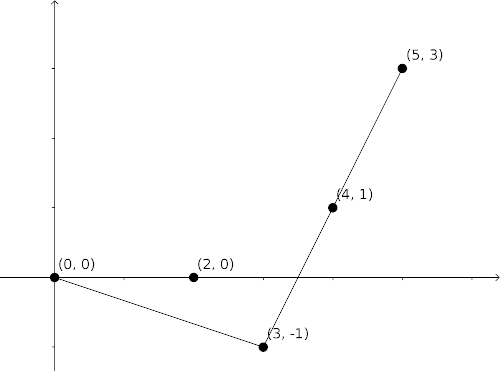
\includegraphics[scale=2.5]{/home/carlo/Tesi/images/figure_4_1}
				\caption{Newton polygon of $f(X) \in \Q_3[X]$}
				\label{figure:figure4.1}
			\end{figure}
		\end{example}
		Let's introduce some basic terms we'll adopt from now on.
		\begin{defn}
			The \emph{vertices} of the Newton polygon are the points $\left(i_j, \ord a_{i_j}\right)$ where the slope changes, the \emph{segments} of the Newton polygon are the segments joining one vertex to the next one; if a segment joins $(i, m)$ to $(i', m')$ its slope is $\tfrac{m' - m}{i' -i}$ and its length is $i' - i$, i.e. the length of its projection onto the horizontal axis.
		\end{defn}
		We have defined the Newton polygon only for a polynomial with constant term $1$, but this doesn't cause loss of generality because the main use of the Newton polygon is to characterize zeroes (and radius of convergence) of $f(X)$. Given a generic $g(X) \in \Cp[X]$ we can write:
		\[
			g(X) = b_kX^k + \dots + b_nX^n = b_k\cdot X^k \cdot \left(1 + \frac{b_{k+1}}{b_k}X + \dots + \frac{b_n}{b_k}X^{n-k}\right) =: b_k \cdot X^k \cdot f(X)
		\]
		and we can study $f(X)$, which satisfies our initial hypothesis.	Before proving our main result about the Newton polygon for polynomials, let's recall what symmetric polynomials are.
		\begin{defn}
			Let $K$ be a commutative ring with unit, $\underline{X} := (X_1, \dots, X_n)$ and let $P(\underline{X}) \in K[\underline{X}]$ be a polynomial in $n$ variables. We say that $P(\underline{X})$ is symmetric if for every $\sigma \in S_n$ we have $P(X_{\sigma(1)}, \dots, X_{\sigma(n)}) = P(X_1, \dots, X_n)$, where $S_n$ is the symmetric group of $n$ elements. \newline
			The symmetric polynomials $\left\{e_i(\underline{X}) : i \in \{0, 1, \dots, n\}\right\}$ defined by
			\begin{gather*}
				e_0(\underline{X}) = 1,\\
				e_k(\underline{X}) = \sum_{1 \leq i_1 < \dots < i_k \leq n} X_{i_1}X_{i_2}\dots X_{i_k}
			\end{gather*}
			are the \emph{elementary symmetric polynomials}.
		\end{defn}
		It is well known that the symmetric polynomials in $n$ variables form a subring $K[\underline{X}]^{S_n}$ and if $P(\underline{X})$ is symmetric then there exists $Q(\underline{Y}) \in K[\underline{Y}]$ such that $P(\underline{X}) = Q(e_1(\underline{X}), \dots, e_n(\underline{X}))$, i.e. the elementary symmetric polynomials ``generate'' all symmetric polynomials.
		It is easy to prove that if $f(X) \in K[X]$ is a monic polynomial of degree $n$ (here we add the hypothesis that $K$ is an integral domain, i.e. there are no divisors of zero) and all its roots are $\alpha_1, \dots, \alpha_n$ then
		\[
			f(X) = \prod_{j=1}^n \left(X - \alpha_j\right) = \sum_{j=0}^n (-1)^{n-j} \cdot e_{n-j}(\alpha_1, \dots, \alpha_n) \cdot X^j,
		\]
		which is a precise relation between the coefficients of $f$ and its roots. Finally we recall that if $f(X) = 1 + \sum_{i=1}^n a_iX^i \in K[X]$ has degree $n$ (here $K$ is a field) and $\alpha_1, \dots, \alpha_n$ are all of its roots, we can write
		\[
		f(X) = \prod_{j=1}^n \left(1 - \frac{X}{\alpha_j}\right) = \sum_{j=0}^n (-1)^j \cdot e_j\left(\frac{1}{\alpha_1}, \dots, \frac{1}{\alpha_n}\right) \cdot X^j;
		\]
		in-fact $f(0) = 1$ and we can divide by $1 = (-1)^na_n\alpha_1\dots\alpha_n$ both sides of $f(X) = a_n(X - \alpha_1)\dots(X - \alpha_n)$.\newline
		We are ready to state and prove the following.
		\begin{thm}
			\label{thm:newton-polygon-polinomial-zeroes}
			Let $f(X) = 1 + \sum_{i=1}^n a_iX^i \in 1 + X\Cp[X]$ be a polynomial of degree $n$, let $\alpha_1, \dots, \alpha_n \in \Cp$ be all of its roots and $\lambda_i := \mathrm{ord}_p\,\left(1/\alpha_i\right)$. If $\lambda$ is a slope of the Newton polygon of $f$ with length $l$, it follows that precisely $l$ of the $\lambda_i$ are equal to $\lambda$. Vice-versa, if $\gamma$ is a \padic order of a reciprocal root then there is a segment of the Newton polygon with slope $\gamma$.
		\end{thm}
		\begin{proof}
			The last statement is trivial if we prove the first one: in-fact the total length of the Newton polygon is $n$ so we have already considered all the roots (counting multiplicity).\newline
			Let's suppose the $\alpha_i$ arranged so that $\lambda_1 \leq \lambda_2 \leq \dots \leq \lambda_n$. Let's suppose that $\lambda_1 = \lambda_2 = \dots = \lambda_r < \lambda_{r+1}$. We then claim that the first segment of the Newton polygon is the one joining $(0,0)$ to $(r, r\lambda_1)$. We know that $a_i = (-1)^i \cdot e_i\left(1/\alpha_1, \dots, 1/\alpha_n\right)$ and, recalling how the $i$-th elementary symmetric polynomial is defined (sum of all possible products of $i$ different variables) and that $\ord(x + y) \geq \min\{\ord(x),\ord(y)\}$, we obtain 
			\[
			\ord(a_i) \geq i\lambda_1,
			\]
			which means that the point $(i, \ord(a_i))$ is on or above the line joining $(0,0)$ to $(r, r\lambda_1)$. Let's now consider $a_r$: only one of the products of $r$ of the $1/\alpha_i$ has \padic order $r\lambda_1$ and it is exactly $1/(\alpha_1 \dots \alpha_r)$, while all the other products have bigger \padic order since they must include at least one $1/\alpha_i$ with $i > r$. Then, by the isosceles triangle principle, $\ord(a_r) = r\lambda_1$. Finally, let's consider $a_i$ with $i > r$: for the same reasoning as before we have $\ord(a_i) > i\lambda_1$. \newline
			All these considerations means exactly that the first segment of the Newton polygon is the one joining $(0,0)$ and $(r, r\lambda_1) = (r, \lambda_1 + \dots + \lambda_r)$. Now, if we have $\lambda_s < \lambda_{s+1} = \dots = \lambda_{s+t} < \lambda_{s+t+1}$ the line joining $(s, \lambda_1 + \dots + \lambda_s)$ to $(s+t, \lambda_1 + \dots + \lambda_s + t\lambda_{s+1})$ is a segment of the Newton polygon. The proof is very similar: if $s \leq i$ then $\ord(a_i) \geq \lambda_1 + \dots + \lambda_s + (i-s)\lambda_{s+1}$, since this is the minimum \padic order in $e_i\left(1/\alpha_1, \dots, 1/\alpha_n\right)$, reached for example by $1/(\alpha_1\dots\alpha_i)$, $\ord(a_{s+t}) = \lambda_1 + \dots + \lambda_s + t\lambda_{s+1}$ by the isosceles triangle principle and if $i > s+t$ then $\ord(a_i) > \lambda_1 + \dots +\lambda_s + (i - s)\lambda_{s+1}$ since we have to choose at least one $1/\alpha_j$ with $j > s+t$.
		\end{proof}
		This theorem, in other words, says that the slopes of the Newton polygon of $f(X)$ are counting with multiplicity the \padic orders of the reciprocal roots of $f(X)$. The aim of the rest of this chapter will be to extend this result to formal power series, but we'll need to do a little more work before. 
	\section{Newton polygons for power series}
		The definition of the Newton polygon for $f(X) \in 1 + X\Cp\ser{X}$ is the same of \cref{defn:newton-polygon-polynomials}: it is the inferior convex hull of all the points in $\Gamma$ (which, this time, will be infinite). Sometimes we'll denote the Newton polygon of $f(X)$ by $\mathfrak{N}(f)$. From now on we'll only consider proper power series, i.e. we'll exclude the case in which $f(X)$ is a polynomial. We can distinguish three different kinds on Newton polygon.
		\begin{enumerate}[label=(\arabic*)]
			\label{enumerate:newton-polygon-types}
			\item We get infinitely many segments of finite length, for example the Newton polygon $f(X) = 1 + \sum_{i=1}^{+\infty} p^{i^2}X^i$ shown in \cref{figure:figure4.2}.
			\item At some point the line we're rotating simultaneously hits infinite points. In this case the Newton polygon has only a finite number of segments, the last one being infinitely long. An example is $f(X) = 1 + \sum_{i=1}^{+\infty} X^i$, whose Newton polygon is simply the horizontal axis.
			\item At some point the line we're rotating has not hit any point yet but it cannot rotate any farther without passing above some points. If this happens, we let the last segment of the Newton polygon have slope equal to the least upper bound of all possible slopes for which the line passes below all the points. A simple example is given by $f(X) = 1 + \sum_{i=1}^{+\infty} pX^i$, whose Newton polygon is the horizontal axis as shown in \cref{figure:figure4.3}.
		\end{enumerate}
		There is a degenerate case of type $(3)$: the vertical line through $(0,0)$ cannot be rotated at all without crossing above some points $(i, \ord a_i)$. An example of this possibility is given by $f(X) = \sum_{i=0}^{+\infty} \tfrac{X^i}{p^{i^2}}$, whose Newton polygon is shown in \cref{figure:figure4.3.1}.
		\begin{figure}
			\centering
			\subfloat[][Newton polygon of type 1 \label{figure:figure4.2}]{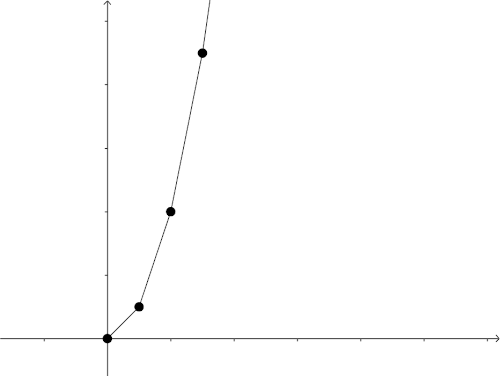
\includegraphics[scale=1.25]{/home/carlo/Tesi/images/figure_4_2}} \qquad \qquad
			\subfloat[][Newton polygon of type 3 \label{figure:figure4.3}]{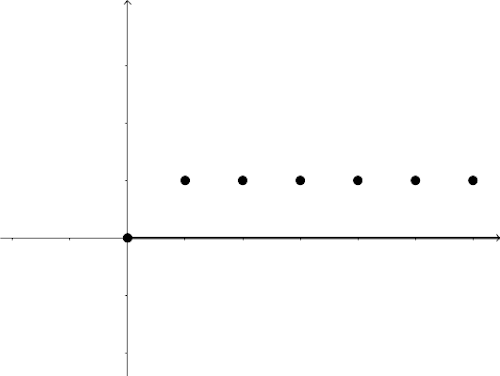
\includegraphics[scale=1.25]{/home/carlo/Tesi/images/figure_4_3}} \\
			\subfloat[][Degenerate Newton polygon \label{figure:figure4.3.1}]{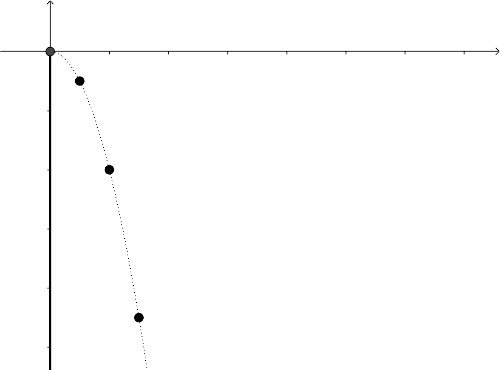
\includegraphics[scale=1.25]{/home/carlo/Tesi/images/figure_4_3_1}} \qquad \qquad
			\subfloat[][Newton polygon of $f(X)$ \label{figure:figure4.4}]{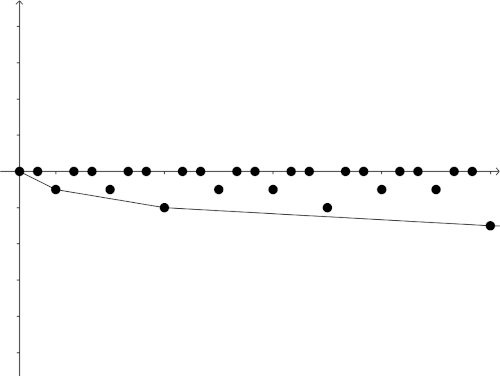
\includegraphics[scale=1.25]{/home/carlo/Tesi/images/figure_4_4}}	
			\caption{Various Newton polygons}		
		\end{figure}
		We'll exclude this case from our study since, as we'll prove in the next proposition, all such series have zero radius of convergence.
		\begin{prop}
			Let $f(X) = 1 + \sum_{i=1}^{+\infty} a_iX^i \in 1 + X\Cp\ser{X}$ be a power series whose Newton polygon is a degenerate case of type $(3)$, i.e. 
			\[
				\forall m \in \R \quad \exists i_m \in \N : \mathrm{ord}_p\, a_{i_m} < m \cdot i_m.
			\]
			Then the radius of convergence of $f$ is $0$.
		\end{prop} 
		\begin{proof}
			We just need to prove that $\limsup\, \pabs{a_n}^{1/n} = +\infty$. Let's define a subsequence of the coefficients $(a_{n_k})_{k \geq 1}$ by induction. We set $n_1 = i_{-1}$ so that $(n_1, \ord a_{n_1})$ lies below the line $y = -x$. Let's now consider the lines $\ell_1$, joining $(0, 0)$ to $(n_1, \ord a_{n_1})$, and $\ell_2$, with equation $y = -2x$: by hypothesis there must be an infinite number of points $(i, \ord a_i)$ lying below both of these two lines. Then there is at least one such point $(j, \ord a_j)$ with $j > n_1$ and we set $n_2 := j > n_1$. We can iterate this procedure (every time we choose $n_k > n_{k-1}$ such that $(n_k, \ord a_{n_k})$ lies below both $y = -kx$ and the line joining $(0,0)$ to $(n_{k-1}, \ord a_{n_{k-1}})$). We have obtained an increasing sequence $(n_k)_{k \geq 1} \subseteq \N$ such that
			\[
				\ord a_{n_k} < -k \cdot n_k \implies \pabs{a_{n_k}}^{1/n_k} > p^k.
			\]
			Using this subsequence we can conclude.
		\end{proof}
		From now on we'll always consider analytic functions with a non-trivial disc of convergence. Before proving general properties of the Newton polygon of analytic functions, let's consider a concrete example.
		\begin{example}
			Let's consider the function $f$ defined by
			\[
				f(X) = \sum_{n=0}^{+\infty} \frac{X^n}{n+1} = \frac{1}{X} \cdot \sum_{n=0}^{+\infty} \frac{X^{n+1}}{n+1} = -\frac{1}{X} \cdot \log_p(1 - X).
			\]
			Looking at the right member it's immediate to see that $f$ converges in $D(1^-)$. If we denote $\ell_i$ the segment joining $\left(p^i-1, -i\right)$ to $\left(p^{i+1}-1, -i-1\right)$ then it's easy to see that the Newton polygon of $f$ is the polygonal line $\bigcup_{i \in \N} \ell_i$ shown in \cref{figure:figure4.4} for $p=3$.
			Assuming that the power series analogue of \cref{thm:newton-polygon-polinomial-zeroes} holds, then, by looking at the Newton polygon of $f$, we would expect to find exactly $p^{i+1} - p^i$ roots having \padic order $1/\left(p^{i+1} - p^i\right)$ for every $i \in \N$ and no other roots. \newline 
			Let's prove this claim: let's fix $j \in \N$ and consider $x = 1 - \zeta$, where $\zeta \in \Cp$ is a primitive $p^{j+1}$-th root of $1$. Then we know by \cref{exercise:7-p.74} that $\ord x = 1/\left(p^{j+1} - p^j\right)$ and that $\log_p(1 - x) = 0$ by \cref{corollary:log-root-of-1} so $f(x) = 0$. Since there are exactly $p^{i+1} - p^i$ primitive roots of $1$, we have found all the predicted roots. Let's now prove that there are no other roots of $f$, i.e. any root is of the form $1 - \xi$ where $\xi$ is a primitive $p^k$-th root of $1$. Let $x \in D(1^-)$ be a root of $f$ and let
			\[
				x_j := 1 - (1 - x)^{p^j}
			\]
			for any $j \in \N$. Using Newton's binomial expansion we get
			\[
				\pabs{x_j} = \pabs{1 - (1 - x)^{p^j}} = \pabs{\sum_{i=1}^{p^j} \binom{p^j}{i} (-x)^i} \leq \pabs{x} < 1,
			\]
			which implies $x_j \in D(1^-)$ for every $j$. We claim that for any $M > 0$ we can find $j_m \in \N$ such that $\pabs{x_{j_m}}< M$. Fixed $M > 0$ we just need to find a $j$ such that
			\[
				\max_{1 \leq i \leq p^j} \pabs{\binom{p^j}{i}x^i} < M.
			\]
			Since $\pabs{x} < 1$ we can find $N \in \N$ such that if $n > N$ then $\pabs{\binom{p^j}{n}x^n} < M$. Now we just need to find a $j$ such that
			\[
					\max_{1 \leq i \leq N} \pabs{\binom{p^j}{i}x^i} < M.
			\]
			Writing $m := \max_{1 \leq i \leq N} (1/\pabs{i!}) > 0$ we have that
			\[
				\pabs{\binom{p^j}{i}} \leq \pabs{\frac{p^j}{i!}} \leq \pabs{p^j} \cdot m
			\]
			and we can conclude, since $\pabs{p^j} \to 0$ as $j \to +\infty$. Now let's consider $j \in \N$ such that $x_j \in D(r_p^-)$; thanks to \cref{prop:exp-and-log-inverse} we have
			\[
				1 - x_j = \exp_p(\log_p(1 - x_j)) =\exp_p\left(p^j\cdot \log_p(1 - x)\right) = \exp_p(0) = 1
			\]
			hence $(1 - x)^{p^j} = 1$ so that $x = 1 - \zeta$ where $\zeta$ is a $p^j$-th root of $1$ and it's one of the roots we already considered. \newline
			We have proved that, for this particular $f(X)$, the power series analogue of \cref{thm:newton-polygon-polinomial-zeroes} holds.
		\end{example}
		Let's now prove a simple but interesting result which explains how we can find the radius of convergence of a series just by looking at its Newton polygon.
		\begin{prop}
			\label{prop:newton-polygon-radius-convergence}
			Let $f(X) = 1 + \sum_{i=1}^{+\infty} a_iX^i \in 1 + X\Cp\ser{X}$ and let $b$ be the least upper bound of all slopes of the Newton polygon of $f$. Then the radius of convergence of $f(X)$ is $p^b$ (if $b=+\infty$ then $f$ converges everywhere).
		\end{prop}
		\begin{proof}
			Let's fix $x \in \Cp$ with $\pabs{x} < p^b$, i.e. $-b' := \ord x > -b$. Then $\ord(a_ix^i) = \ord a_i -ib'$ but, since $b' < b$, it's clear that sufficiently far out all the points $(i, \ord a_i)$ will lie arbitrarily far above $(i, b'i)$, see \cref{figure:figure4.5}. This means exactly $\lim_{i\to +\infty} \ord(a_ix^i) = +\infty$, i.e. $f(X)$ converges at $x$. \begin{figure}
				\centering
				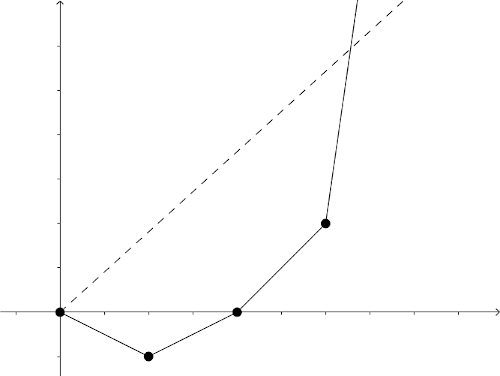
\includegraphics[scale=1.5]{/home/carlo/Tesi/images/figure_4_5}
				\caption{Case $\protect\pabs{x} < p^b$} % Workaround, it works
				\label{figure:figure4.5}
			\end{figure}
			Let's now consider the case $\pabs{x} > p^b$, i.e. $-b' := \ord x < -b$. Since $b' > b$ we find an infinite number of $i \in \N$ such that $\ord(a_ix^i) = \ord a_i - ib' < 0$ which implies that $f(X)$ does not converge at $x$. We can then conclude that the radius of convergence of $f$ is exactly $p^b$.
		\end{proof}
		Obviously this proposition doesn't tell us anything about the convergence of $f(X)$ at the radius of convergence, i.e. if $\pabs{x} = p^b$. 
		\begin{prop}
			\label{prop:newton-polygon-circonference-convergence}
			Let $f(X) = 1 + \sum_{i=1}^{+\infty} a_iX^i \in 1 + X\Cp\ser{X}$ be an analytic power series with radius of convergence $r=p^b$, where $b$ is the least upper bound of the slopes of the Newton polygon. Then $f(X)$ converges on $D(r)$ if and only if $\mathfrak{N}(f)$ is of type $(3)$ (see the beginning of \cref{enumerate:newton-polygon-types}) and $\lim_{i \to +\infty} d_i = +\infty$, where $d_i$ is the distance between $(i, \mathrm{ord}_p\, a_i)$ and the last line of $\mathfrak{N}(f)$.
		\end{prop}
		\begin{proof}
			If $b \notin \Q$ there's nothing to prove since no element of $\Cp$ can have order $b$; from now on we'll assume $b \in \Q$.
			First of all we prove that if the Newton polygon of $f$ is of type $(1)$ or $(2)$ then $f(X)$ does not converge if $\pabs{x} = p^b$. \newline 
			Let's first consider a Newton polygon of type $(1)$ and let $\Lambda$ be the set of all its slopes. Then $b = \sup \Lambda$ and if $b = +\infty$ there's nothing to prove. If $b < +\infty$ then there exists $y_0 \in \R$ such that $\ell\colon y = y_0 + bx$ is an ``asymptote'' of the Newton polygon, see \cref{figure:figure-extra-1} (the slopes are increasing and their $\sup$/$\lim$ is $b$). Then we can consider the vertices of the Newton polygon, indexed by $\left(i_j\right)_{j \in \N}$. It is clear that the distance $d_j$ between $\left(i_j, \ord a_{i_j}\right)$ and $\ell$ tends to $0$ and so does $\left(\ord a_{i_j} - i_jb\right)$, which is equal to $d_j/\cos(\arctan b)$ (if $b=0$ then it is equal to $d_j$). If $\pabs{x} = p^b$ then $\ord x = -b$ so $\ord(a_ix^i) = \ord a_i - ib$. We then conclude that $\ord(a_ix^i) \not\to +\infty$ when $i \to +\infty$, i.e. $f$ does not converge at $x$. 
			Instead if $f$ has a Newton polygon of type $(2)$ then $b$ is its final slope and, by definition, there are infinite points on this final segment. This means that if we call the final line $\ell\colon y_0 + bx$ then we can find an increasing subsequence $\left(i_j\right)_{j \in \N} \subseteq \N$ such that $\ord a_{i_j} = y_0 + i_jb$ so $\ord\left(a_{i_j}x^{i_j}\right) = y_0 \not\to +\infty$ and we can conclude that there's no convergence in $x$.\newline
			Let's now suppose that $\mathfrak{N}(f)$ is of type $(3)$ and $x \in \Cp$ with $\pabs{x} = p^b$. Then $f(X)$ converges in $x$ if and only if $\lim_{i \to +\infty} \ord\left(a_ix^i\right) = +\infty$; as before, with a little trigonometry, we have
			\begin{gather*}
				\ord\left(a_ix^i\right) = \ord a_i - ib = 
				\begin{cases}
					d_i, & \text{if $b=0$;} \\
					\frac{d_i}{\cos(\arctan b)}, & \text{otherwise;} 
				\end{cases}
			\end{gather*}
			and we can conclude (by hypothesis $\lim_{i \to +\infty} d_i = +\infty$). An example is $f(X) = 1 + \sum_{i=1}^{+\infty} 2^iX^{2^i} \in 1 + X\C_2\ser{X}$, whose Newton polygon is shown in \cref{figure:figure4.5.1}.
			\begin{figure}
				\centering
				\subfloat[][Newton polygon with an asymptote \label{figure:figure-extra-1}]{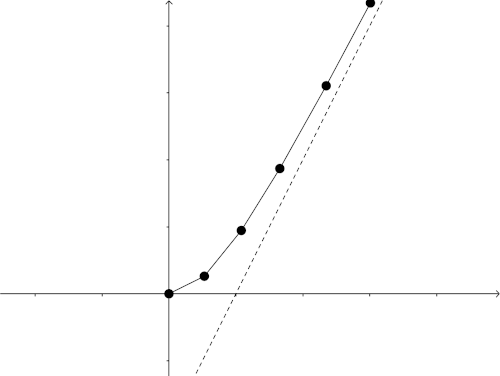
\includegraphics[scale=1.25]{/home/carlo/Tesi/images/figure_extra_1}} \qquad
				\subfloat[][Newton polygon with convergence at border \label{figure:figure4.5.1}]{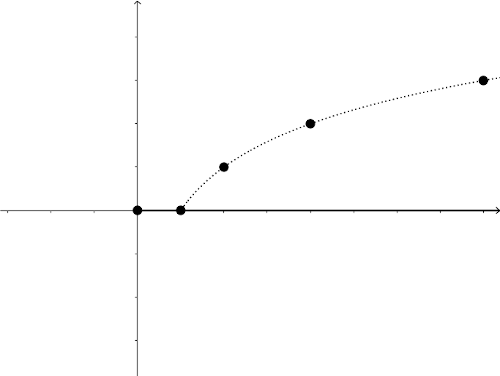
\includegraphics[scale=1.25]{/home/carlo/Tesi/images/figure_4_5_1}}
				\caption{Two other types of Newton polygons}
			\end{figure}
		\end{proof}
		Let's introduce a useful trick we'll often use in the next proofs.
		\begin{lemma}
			\label{lemma:newton-polygon-translation}
			Let $c \in \Cp^\times$ with $\mathrm{ord}_p\, c = \lambda$, $f(X) = 1 + \sum_{i=1}^{+\infty} a_iX^i \in 1 + X\Cp\ser{X}$ and $g(X) := f\left(X/c\right)$. Then the Newton polygon of $g$ is obtained subtracting the line $y = \lambda x$ to the Newton polygon of $f$.
		\end{lemma}
		\begin{proof}
			If we write $g(X) = 1 + \sum_{i=1}^{+\infty} b_iX^i$ then it's immediate that $b_i = a_i/\left(c^i\right)$ so $\ord b_i = \ord a_i - i\lambda$ and we can conclude.
		\end{proof}
		We'll now prove four technical lemmas we'll then use to prove our final result.
		\begin{lemma}
			\label{lemma:lemma6-p.102}
			Let $f(X) = 1 + \sum_{i=1}^{+\infty} a_iX^i \in 1 + X\Cp\ser{X}$ and suppose that $\lambda_1$ is the first slope of its Newton polygon. Let $c \in \Cp$ with $\mathrm{ord}_p\,c = \lambda \leq \lambda_1$ and assume that $f(X)$ converges on the closed disc $D(p^{\lambda})$ (this automatically happens if $\lambda < \lambda_1$ or if the Newton polygon has more than one segment). Let 
			\[
				g(X) = (1 - cX)f(X) \in 1 + X\Cp\ser{X}.
			\]
			Then $\mathfrak{N}(g)$ is obtained by joining $(0,0)$ to $(1, \lambda)$ and then translating $\mathfrak{N}(f)$ by $\vec{v} = (1, \lambda)$ ($1$ to the right and $\lambda$ upwards). If $\mathfrak{N}(f)$ has last slope $\lambda_f$ and $f(X)$ converges on $D(p^{\lambda_f})$ then $g(X)$ also converges on $D(p^{\lambda_f})$. Conversely, if $g(X)$ converges on $D(p^{\lambda_f})$ then so does $f(X)$.
		\end{lemma}
		\begin{proof}
			A graphic interpretation of the lemma can be found at \cref{figure:figure4.6}.
			\begin{figure}
				\centering
				\subfloat[][Newton polygon of $f_1(X)$]{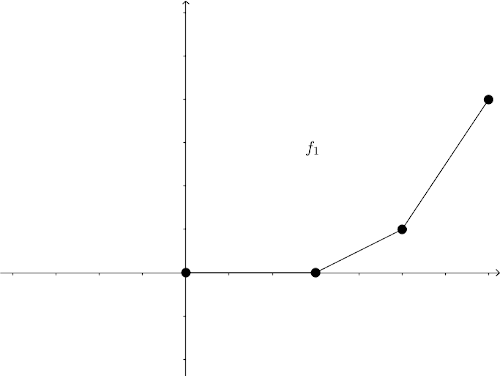
\includegraphics[scale=1.25]{/home/carlo/Tesi/images/figure_4_6_1}} \qquad \qquad \subfloat[][Newton polygon of $g_1(X)$]{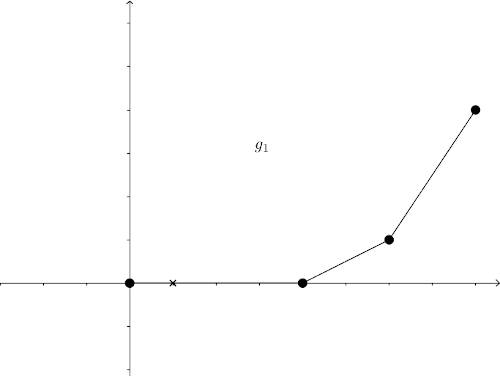
\includegraphics[scale=1.25]{/home/carlo/Tesi/images/figure_4_6_2}} \\
				\subfloat[][Newton polygon of $f(X)$]{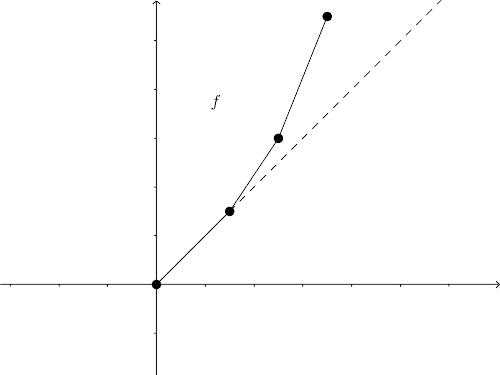
\includegraphics[scale=1.25]{/home/carlo/Tesi/images/figure_4_6_3}} \qquad \qquad
				\subfloat[][Newton polygon of $g(X)$]{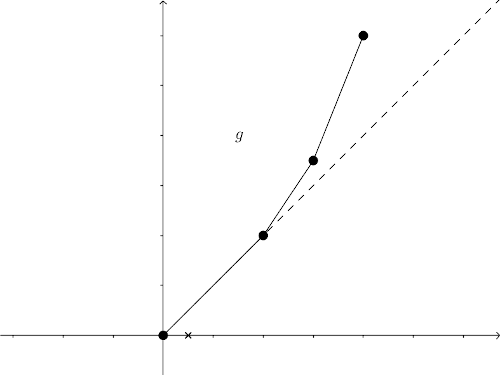
\includegraphics[scale=1.25]{/home/carlo/Tesi/images/figure_4_6_4}} 
				\caption{Example of \protect\cref{lemma:lemma6-p.102}}
				\label{figure:figure4.6}
			\end{figure}
			We can consider only the special case $c=1, \lambda = 0$. In-fact, let's suppose the lemma holds for this case and let $f(X)$ and $g(X)$ as in the statement. Then $f_1(X) := f\left(\tfrac{X}{c}\right)$ and $g_1(X) := (1 - X)f_1(X)$ satisfy our hypothesis (with the parameters $\underline{c}=1, \underline{\lambda} = 0, \underline{\lambda_1} = \lambda_1 - \lambda$, by \cref{lemma:newton-polygon-translation}). Thus, since we're assuming the lemma to be true if $c=1$, we know the shape of the Newton polygon of $g_1(X)$ (and the convergence of $g_1(X)$ on $D(p^{\lambda_f - \lambda})$ when $f$ converges on $D(p^{\lambda})$). Now, $g(X) = g_1(cX)$ so,  using again \cref{lemma:newton-polygon-translation}, we obtain the desired information about the Newton polygon of $g(X)$ (and the desired convergence, which is immediate). So we can just prove the lemma when $c = 1$.\newline
			If $g(X) = 1 + \sum_{i=1}^{+\infty} b_iX^i$ then, since by definition $g(X) = (1 - X)f(X)$, we have $b_{i+1} = a_{i+1} - a_i$ for $i \geq 0$ (clearly $a_0 = 1$). Then
			\begin{equation*}
				\ord b_{i+1} \geq \min\left\{\ord a_{i+1}, \ord a_i \right\} \tag{$\star$}
			\end{equation*}
			and the equality holds when $\ord a_{i+1} \neq \ord a_i$. It is easy to see that both $(i, \ord a_i)$ and $(i, \ord a_{i+1})$ lie on or above the Newton polygon of $f(X)$ and so does $(i, \ord b_{i+1})$, by $(\star)$. If $(i, \ord a_i)$ is a vertex then necessarily $\ord a_{i+1} > \ord a_i$ so $\ord b_{i+1} = \ord a_i$. This means exactly that the Newton polygon of $g(X)$ has the shape described in the lemma, as far as the last vertex of $f(X)$. If $\mathfrak{N}(f)$ is of type $(1)$ we can conclude here: there is no last vertex and no last slope. It remains only to show that when $\mathfrak{N}(f)$ has last slope $\lambda_f$ then also $\mathfrak{N}(g)$ does and if $f(X)$ converges on $D(p^{\lambda_f})$ then so does $g(X)$. We already know $\ord b_{i+1} \geq \min\left\{\ord a_{i+1}, \ord a_i \right\}$ so $g(X)$ converges wherever $f(X)$ does; then if $\lambda_g$ is the least upper bound of the slopes of $\mathfrak{N}(g)$ we have $\lambda_g \geq \lambda_f$ (by \cref{prop:newton-polygon-radius-convergence}). We must only rule out the case $\lambda_g > \lambda_f$. If it were the case, then, for some large $i$, the point $(i+1, \ord a_i)$ would lie below $\mathfrak{N}(g)$ so we'd have $\ord b_j > \ord a_i$ for every $j  \geq i+1$ (this holds in this particular case where $\lambda = 0$ since $0 \leq \lambda_1 \leq \lambda_f < \lambda_g$). Using $j = i+1$ we obtain $\ord a_{i+1} = \ord a_i$ because $a_{i+1} = b_{i+1} + a_i$. Then, using $j = i+2$, we obtain $\ord a_{i+2} = \ord a_{i+1} = \ord a_i$ and so on for every $j$. This means $\ord a_j = \ord a_i$ for every $j \geq i$ and contradicts the assumed convergence of $f(X)$ on $D(1) \subseteq D(p^{\lambda_f})$. Then we must have $\lambda_g = \lambda_f$ and $\mathfrak{N}(g)$ is exactly of the predicted shape. This implies in particular that if $f(X)$ converges on $D(p^{\lambda_f})$ then so does $g(X)$ (see \cref{prop:newton-polygon-circonference-convergence}). The converse assertion, i.e. convergence of $g(X)$ implies convergence of $f(X)$, can be proved in an analogue way.
		\end{proof}
		\begin{lemma}
			\label{lemma:lemma7-p.103}
			Let $f(X) = 1 + \sum_{i=1}^{+\infty} a_iX^i \in 1 + X\Cp\ser{X}$ have Newton polygon with first slope $\lambda_1$. Let's assume that $f(X)$ converges on $D\left(p^{\lambda_1}\right)$ and that the line $\ell\colon y = \lambda_1x$ actually passes through a point $(i, \mathrm{ord}_p\, a_i)$ with $i \geq 1$ (both of these conditions are automatically satisfied if $\mathfrak{N}(f)$ has more than one slope). Then there exists an $x \in \Cp$ for which $\mathrm{ord}_p\, x = -\lambda_1$ and $f(x) = 0$.
		\end{lemma}
		\begin{proof}
			Let's first consider the case $\lambda_1 = 0$ and then reduce the general case to this one. If $\lambda_1 = 0$ we have $\ord a_i \geq 0$ for every $i \in \N$ and $\lim_{i \to +\infty} \ord a_i = +\infty$ since $f(X)$ converges on $D(1)$. Let $N := \max \left\{i \in \N^\times : \ord a_i=0 \right\}$ and let $f_n(X) := 1 + \sum_{i=1}^n a_iX^i \in 1 + X\Cp[X]$. By \cref{thm:newton-polygon-polinomial-zeroes}, if $n \geq N$ then the polynomial $f_n(X)$ has precisely $N$ roots with \padic order $0$, let them be $x_{n, 1}, \dots, x_{n, N}$ (it's immediate that $\mathfrak{N}(f_n)$ has a first segment with slope $0$ and length $N$). Let's define a sequence: $x_N := x_{N, 1}$ and, for $n \geq N$, $x_{n+1} := x_{n+1, i}$ where $i$ is such that  $\pabs{x_{n+1, i} - x_n}$ is minimal. We claim that $\left(x_n\right)_{n \geq N} \subseteq \Cp$ is Cauchy and its limit $x$ is the desired root of $f$. If $S_n$ denotes the set containing the roots of $f_n(X)$, counted with multiplicity, for $n \geq N$ we have
			\[
				\pabs{f_{n+1}(x_n) - f_n(x_n)} = \pabs{f_{n+1}(x_n)} = \prod_{\alpha \in S_{n+1}} \pabs{1 - \frac{x_n}{\alpha}}
			\]
			where we used $f_n(x_n) = 0$ and $f_{n+1}(X) = \prod_{\alpha \in S_{n+1}} \left(1 - \tfrac{X}{\alpha}\right)$. It's clear that if $\alpha \in S_{n+1}$ then $\ord \alpha \leq 0$: in-fact we cannot have $\ord \alpha > 0$ and $f_{n+1}(\alpha) = 0$ by the isosceles triangle principle (recall that $\ord a_i \geq 0$). Now if $\alpha \in S_{n+1}$ has $\ord \alpha < 0$ then $\pabs{1 - \tfrac{x_n}{\alpha}} = 1$, since $\pabs{x_n} = 1$. Then we can write
			\[
				\pabs{f_{n+1}(x_n) - f_n(x_n)} = \prod_{i=1}^N \pabs{1 - \frac{x_n}{x_{n+1, i}}} = \prod_{i=1}^N \pabs{x_{n+1, i} - x_n} \geq \pabs{x_{n+1} - x_n}^N,
			\]
			by the choice of $x_{n+1}$. We have obtained
			\[
				\pabs{x_{n+1} - x_n}^N \leq \pabs{f_{n+1}(x_n) - f_n(x_n)} = \pabs{a_{n+1}x_n^{n+1}} = \pabs{a_{n+1}} 
			\]
			so $\lim_{n \to +\infty} \pabs{x_{n+1} - x_n}^N = 0$ (by hypothesis $\lim_{n \to +\infty} \pabs{a_{n+1}} = 0$) and we have proved that $\left(x_n\right)_{n \geq N}$ is Cauchy (see \cref{lemma:cauchy-sequence-ultrametric}). Since $\Cp$ is complete there exists $x := \lim_{n \to +\infty} x_n$ and, by continuity of $\pabs{\ }$, we have $\pabs{x} = 1$. It's clear that for any $y \in D(1)$ we have $\lim_{n \to +\infty} f_n(y) = f(y)$ (the \padic absolute value of the difference tends to zero) so we have $f(x) = \lim_{n \to +\infty} f_n(x)$. Now,
			\[
				\pabs{f_n(x)} = \pabs{f_n(x) - f_n(x_n)} = \pabs{x - x_n}\cdot\pabs{\sum_{i=1}^n a_i\frac{x^i - x_n^i}{x - x_n}} \leq \pabs{x - x_n}
			\]
			because $\pabs{a_i} \leq 1$ and $\pabs{\tfrac{x^i - x_n^i}{x - x_n}} = \pabs{x^{i-1} + x^{i-2}x_n + \dots + x_n^{i-1}} \leq 1$. Hence we can conclude that $f(x) = \lim_{n \to +\infty} f_n(x) = 0$ and we have proved the lemma if $\lambda_1 = 0$.\newline
			The general case follows easily. Let $\pi \in \Cp$ be any number with $\ord \pi = \lambda_1$. Clearly such a $\pi$ exists: for example, if $(i, \ord a_i)$ lies on $y=\lambda_1x$ and $i \geq 1$ (such a point exists by assumption) then $\pi$ can be any $i$-th root of $a_i$ (recall that $\Cp$ is algebraically closed). Now let $g(X) := f\left(X/\pi\right)$; it's clear by \cref{lemma:newton-polygon-translation} that $g(X)$ satisfies the conditions of the lemma with $\lambda_1 = 0$. Then we already 
			know that there exists $x_0$ with $\ord x_0 = 0$ such that $g(x_0) = 0$. Then if $x = x_0/\pi$ we have $\ord x = -\lambda_1$ and $f(x) = f\left(x_0/\pi\right) = g(x_0) = 0$.
		\end{proof}
		\begin{lemma}
			\label{lemma:lemma8-p.105}
			Let $f(X) = 1 + \sum_{i=1}^{+\infty} a_iX^i \in 1 + X\Cp\ser{X}$ and let $\alpha \in \Cp$ such that $f(\alpha) = 0$. Let $g(X)$ be obtained by dividing $f(X)$ by $1 - \tfrac{X}{\alpha}$. Then $g(X)$ converges on $D(\pabs{\alpha})$.
		\end{lemma}
		\begin{proof}
			First of all, let's observe that $\alpha \neq 0$ and that dividing $f(X)$ by $1 - \tfrac{X}{\alpha}$ is the same thing of multiplying $f(X)$ by the geometric series $\sum_{i=0}^{+\infty} \left(\tfrac{X}{\alpha}\right)^i$. Let's write $g(X) = 1 + \sum_{i=1}^{+\infty} b_iX^i$ and let $f_n(X) := 1 + \sum_{i=1}^n a_iX^i$ be the $n$-th partial sum of $f(X)$. By an easy computation we infer that
			\[
				b_i = \sum_{j=0}^i \frac{a_j}{\alpha^j}
			\]
			where we set $a_0 = 1$. Then it's easy to see that
			\[
				b_i\alpha^i = f_i(\alpha)
			\]
			hence $\pabs{b_i\alpha^i} = \pabs{f_i(\alpha)} \to 0$ as $i \to +\infty$, since $f(\alpha) = 0$ and $f(x) = \lim_{n \to +\infty}f_n(x)$ wherever $f$ converges. This means exactly that $g(X)$ converges on $D(\pabs{\alpha})$.
		\end{proof}
		\begin{lemma}
			\label{lemma:order-zeroes-function}
			Let $f(X) = 1 + \sum_{i=1}^{+\infty} a_iX^i \in 1 + X\Cp\ser{X}$ such that $\lambda$ is the first slope of $\mathfrak{N}(f)$ and $f$ converges on some disc $D$. If $\alpha \in D$ is a root of $f$, i.e. $f(\alpha) = 0$, then $\mathrm{ord}_p\, \alpha \leq -\lambda$. If $\lambda$ is the only slope of $\newt{f}$ and no point of $\newt{f}$ lies on $y=\lambda x$, then $\mathrm{ord}_p\,\alpha < -\lambda$.
		\end{lemma}
		\begin{proof}
			Let's suppose that $\alpha \in D$ is such that $\ord \alpha = -\lambda' > -\lambda$. We have
			\[
				\ord(a_i\alpha^i) = \ord a_i -i\lambda' > \ord a_i -i\lambda \geq 0,
			\]
			where we used that all the points $(i, \ord a_i)$ lie on or above the line $y=\lambda x$ (by definition of Newton polygon). Then we have $\ord 1 = 0$ and $\ord(a_i\alpha^i) > 0$ for $i \geq 1$ and so $\alpha$ cannot be a root of $f$. The last statement can be proved with an analogue reasoning.
		\end{proof}
		Finally we are ready to prove the main theorem of this section which will imply, as a corollary, the power series analogue of \cref{thm:newton-polygon-polinomial-zeroes}.
		\begin{thm}[\padic Weierstrass Preparation Theorem]
			\label{thm:weierstrass-padic-preparation}
			Let $f(X) = 1 + \sum_{i=1}^{+\infty} a_iX^i \in 1 + X\Cp\ser{X}$ converge on $D(p^{\lambda})$. Let $N$ be the total horizontal length of all segments in $\mathfrak{N}(f)$ having slope less or equal to $\lambda$ if this length is finite $($i.e. if $\mathfrak{N}(f)$ hasn't an infinitely long last segment of slope $\lambda)$. On the other hand, if the Newton polygon of $f$ has last slope $\lambda$, then let $N$ be the greatest index $i$ such that $(i, \ord a_i)$ lies on that final segment $($there must be such a final index since $f$ converges on $D(p^{\lambda}))$. Then there exists a polynomial $h(X) \in 1 + X\Cp[X]$ of degree $N$ and a power series $g(X) = 1 + \sum_{i=1}^{+\infty} b_iX^i$, which converges and is non-zero on $D(p^{\lambda})$, such that
			\[
				h(X) = f(X) \cdot g(X).
			\]
			The polynomial $h(X)$ is uniquely determined by these properties and $\mathfrak{N}(h)$ coincides with $\mathfrak{N}(f)$ up to $x = N$.
		\end{thm}
		\begin{proof}
			We use induction on $N$. Let's first consider the basic case $N = 0$, where the first slope of $\mathfrak{N}(f)$ is greater or equal to $\lambda$. In this case it's evident that we can assume $\lambda \in \Q$ without loss of generality. We have to show that $g(X) = 1/f(X)$ converges and is non-zero on $D(p^{\lambda})$ (recall that any power series with a non-zero constant term is invertible). We can only consider the special case $\lambda = 0$. In-fact, let $f(X) \in 1 + X\Cp\ser{X}$ converge on $D(p^{\lambda})$: we can choose $c \in \Cp$ with $\ord c = \lambda$ using \cref{prop:qpa-every-order} (we assumed $\lambda \in \Q$) and then define $\tilde{f}(X) := f\left(\tfrac{X}{c}\right)$. Now, $\tilde{f}$ converges on $D(1)$ and if $\lambda = 0$ then $N = 0$, i.e. the first slope of its Newton polygon is greater or equal to $0$ by \cref{lemma:newton-polygon-translation}. So, assuming the theorem holds when $N = \lambda = 0$ we infer that there exists $\tilde{g}(X) \in 1 + X\Cp\ser{X}$ which converges and is non-zero on $D(1)$ such that $1 = \tilde{f}(X)\cdot\tilde{g}(X)$. Using $cX$ in place of $X$ we obtain $1 =f(X) \cdot \tilde{g}(cX)$ and it's immediate that $g(X) := \tilde{g}(cX)$ has all the desired properties. So we can only consider the special case $\lambda = 0$. Thus, we can suppose $\ord a_i > 0$ for every $i \in \N$ and $\lim_{i \to +\infty} \ord a_i = +\infty$ (we have convergence on $D(1)$). It's easy to obtain the following equality for the coefficients of $g(X) = 1/f(X)$:
			\[
				b_i = -\left(\sum_{j=1}^i b_{i-j}a_j \right),
			\]
			where we set $b_0 = 1$. From an easy induction on $i$ it follows that $\ord b_i > 0$ for $i \geq 1$. This implies that the first slope of $\mathfrak{N}(g)$ is greater than $0$ (or it's equal to $0$ but with no points on it) and, by \cref{lemma:order-zeroes-function}, we know that $g$ doesn't have roots on $D(1)$. Now it remains only to show that $g(X)$ actually converges on $D(1)$, i.e. that $\lim_{i \to +\infty} \ord b_i = +\infty$. Let's fix $M > 0$: we can find $m \in \N$ such that $i > m$ implies $\ord a_i > M$. Now if
			\[
				\epsilon := \min_{1 \leq j \leq m} \ord a_j> 0
			\]
			we claim that $i > nm$ implies $\ord b_i > \min\{M, n\epsilon\}$, from which it easily follows $\ord b_i \to +\infty$ as $i \to +\infty$. We'll prove this claim by induction on $n$. We have already proved the case $n = 0$. Now, let's suppose $n \geq 1$ and that the claim holds for $n - 1$; if $i > nm$ we have
			\[
				b_i = -\left(b_{i-1}a_i + \dots + b_{i-m}a_m + b_{i-(m+1)}a_{m+1} + \dots + a_1 \right).
			\]
			The terms $b_{i-j}a_j$ with $j > m$ have \padic order greater than $M$, while if $j \geq m$ we have $\ord(b_{i-j}a_j) \geq \ord b_{i-j} + \epsilon$ and, since $i - j > (n-1)m$, by inductive hypothesis we obtain
			\[	
				\ord(b_{i-j}a_j) \geq \ord b_{i-j} + \epsilon > \min\{M, (n-1)\epsilon\} + \epsilon.
			\]
			This proves our claim, hence the theorem when $N = 0$ (the statement about the Newton polygon here is trivial since $h(X) = 1$).\newline
			Now let's consider the general case with $N \geq 1$ and suppose that the theorem holds for $N - 1$. Let $\lambda_1 \leq \lambda$ be the first slope of $\mathfrak{N}(f)$; if it is the only slope then, since $N \geq 1$, there's at least one point on $y = \lambda_1x$. We can then use \cref{lemma:lemma7-p.103} to find $\alpha$ such that $f(\alpha) = 0$ and $\ord \alpha = -\lambda_1$. Let's define
			\[
				f_1(X) := \frac{f(X)}{1 - \frac{X}{\alpha}} = f(X) \cdot \sum_{j=0}^{+\infty} \left(\frac{X}{\alpha}\right)^j \in 1 + X\Cp\ser{X}.
			\]
			By \cref{lemma:lemma8-p.105}, $f_1$ converges on $D(p^{\lambda_1})$. Setting $c := \tfrac{1}{\alpha}$ we have $f(X) = (1 - cX)\cdot f_1(X)$. Let $\lambda_1'$ be the first slope of $\mathfrak{N}(f_1)$; it must necessarily be $\lambda_1' \geq \lambda_1$. In-fact $\lambda_1' < \lambda_1$ implies that $\mathfrak{N}(f_1)$ has more than one slope and that, by \cref{lemma:lemma7-p.103}, $f_1$ has a root with \padic order $-\lambda_1'$ and so does $f$, but this is impossible by \cref{lemma:order-zeroes-function} since $-\lambda_1' > -\lambda_1$. We can now apply \cref{lemma:lemma6-p.102}, with parameters $\underline{f} = f_1, \underline{g} = f, \underline{\lambda} = \lambda_1, \underline{\lambda_1} = \lambda_1'$ and we get that $\mathfrak{N}(f_1)$ is obtained translating $\mathfrak{N}(f) \setminus \ell((0,0), (1, \lambda_1))$ by $\vec{v} = (-1, -\lambda_1)$, where $\ell(P, Q)$ is the segment joining $P$ to $Q$. We claim that $f_1$ converges on $D(p^{\lambda})$: if $\lambda$ isn't the final slope of $\mathfrak{N}(f)$ then it's trivially true, otherwise \cref{lemma:lemma6-p.102} tells us that when $\mathfrak{N}(f)$ has last slope $\lambda$ and $f$ converges on $D(p^{\lambda})$ then so does $f_1$. Thus, $f_1$ satisfies all the conditions of the theorem with $N-1$ instead of $N$ (recall that, to obtain $\mathfrak{N}(f_1)$, we removed a segment with slope $\lambda_1 \leq \lambda$ and with length $1$ from $\mathfrak{N}(f)$). By inductive hypothesis we can find $h_1(X) \in 1 + X\Cp[X]$ of degree $N-1$ and a series $g(X) \in 1 + X\Cp\ser{X}$, convergent and non-zero on $D(p^{\lambda})$, such that
			\[
				h_1(X) = f_1(X) \cdot g(X).
			\]
			Multiplying both sides by $(1 - cX)$ and setting $h(X) := (1 - cX)h_1(X)$ we obtain
			\[
				h(X) = f(X) \cdot g(X),
			\]
			where $h$ and $g$ have the desired properties. Let's also observe that $\mathfrak{N}(h_1)$ coincides with $\mathfrak{N}(f_1)$ up to $x = N-1$ and that, since $h(X) = (1 - cX)h_1(X)$, $\mathfrak{N}(h)$ is obtained joining $(0,0)$ to $(1, \lambda_1)$ and then translating $\mathfrak{N}(h_1)$. Then it's clear that $\mathfrak{N}(h)$ will coincide with $\mathfrak{N}(f)$ up to $x = N$.\newline 
			Now we have only to prove the uniqueness of $h(X)$ (we have only proved its existence).
			Let's suppose that $\tilde{h}(X) \in 1 + X\Cp[X]$ is another polynomial of degree $N$ such that \[
				\tilde{h}(X) = f(X) \cdot g_1(X),
			\]
			where $g_1(X) \in 1 + X\Cp\ser{X}$ converges and is non-zero on $D(p^{\lambda})$. We have
			\[
				\tilde{h}(X)\cdot g(X) = f(X)\cdot g(X) \cdot g_1(X) = h(X) \cdot g_1(X). \tag{$*$}
			\]
			To prove uniqueness it suffices to show that $(*)$ implies that $h$ and $h_1$ have the same roots with the same multiplicities (they both have constant term $1$). The case $N=1$ is trivial. Let's now consider $N > 1$. The polynomial $h(X)$ is the one we built before so we already know that $\mathfrak{N}(h)$ coincides with $\mathfrak{N}(f)$ up to $x = N$. Using \cref{thm:newton-polygon-polinomial-zeroes}, this means that every root of $h(X)$ is in $D(p^{\lambda})$ (by assumption all the slopes of $\mathfrak{N}(h)$ are less or equal to $\lambda$). Let $\alpha \in \Cp$ be a root of $h(X)$. Since $\alpha \in D(p^{\lambda})$ we can compute $g(\alpha)$ and $g_1(\alpha)$ and, by hypothesis, they're not zero. So $\alpha$ must also be a root of $\tilde{h}(X)$. Let's define 
			\[
				\tilde{k}(X) := \frac{\tilde{h}(X)}{1 - \frac{X}{\alpha}}, \qquad k(X) := \frac{h(X)}{1 - \frac{X}{\alpha}};
			\]
			they're two polynomials in $1 + X\Cp[X]$ of degree $N - 1$ satisfying $\tilde{k}(X)\cdot g(X) = k(X)\cdot g_1(X)$. We can repeat this process with every other root of $h(X)$ and, at the end, both polynomials will be $1$ so we have proved uniqueness.
		\end{proof}
		This is a very powerful theorem, with a lot of interesting corollaries.
		\begin{corollary}
			\label{corollary:newton-polygon-zeroes}
			If a segment of the Newton polygon of $f(X) \in 1 + X\Cp\ser{X}$ has finite length $N$ and slope $\lambda$, then there are exactly $N$ values of $x$ (counting multiplicity) for which $f(x) = 0$ and $\mathrm{ord}_p\, x = -\lambda$.
		\end{corollary}
		\begin{proof}
			It is an immediate application of \cref{thm:weierstrass-padic-preparation} and \cref{thm:newton-polygon-polinomial-zeroes}. 
		\end{proof}
		\begin{example}
			We can use the Newton polygon to study the exact region of convergence of $\E_p(X)$, the Artin-Hasse exponential (see \cref{defn:artin-hasse}). We already know, by \cref{prop:artin-hasse-formula} and \cref{prop:artin-hasse-formula}, that
			\[
				\E_p(X) = \exp_p\left(\sum_{i=0
				}^{+\infty} \frac{X^{p^i}}{p^i}\right)
			\]
			and that $\E_p(X)$ converges on $D(1^-)$. We'll show that this is the exact region of convergence, i.e. that $\E_p(X)$ doesn't converge if $\pabs{x} = 1$. Let's define
			\[
				f(X) = \sum_{i=0}^{+\infty} \frac{X^{p^i -1}}{p^i} \in 1 + X\Cp\ser{X},
			\]
			so that $\E_p(X) = \exp_p(X \cdot f(X))$. Now, $\E_p(X)$ converges at $x \in \Cp$ if and only if $x\cdot f(x) \in D(r_p^-)$. We'll show that $f(X)$ doesn't even converge if $\pabs{x} = 1$. Writing $f(X) = 1 + \sum_{n=1}^{+\infty} a_iX^i$, it's immediate that
			\begin{gather*}
				(i, \ord a_i) =
				\begin{cases}
					\left(p^k - 1, -k\right), & \text{if $\exists k \in \N$ such that $i = p^k - 1$;} \\
					(i, 0), & \text{otherwise;}
				\end{cases}.
			\end{gather*}
			If $\ell_i$ is the segment joining $\left(p^i-1, -i\right)$ to $\left(p^{i+1}-1, -i-1\right)$ then we have $\mathfrak{N}(f) = \bigcup_{i \in \N} \ell_i$ (see \cref{figure:figure-extra-2} for $p=2$). It is clearly a type $(1)$ polygon (infinite number of finite segments). The segment $\ell_i$ has slope $\lambda_i =- \tfrac{1}{p^i(p - 1)} < 0$ and we have $\lim_{i \to +\infty} \lambda_i = 0$. This proves that $0$ is the least upper bound of all slopes of $\mathfrak{N}(f)$ so, using \cref{prop:newton-polygon-radius-convergence}, we can conclude: the radius of convergence of $f$ is $1 = p^0$ and we cannot have convergence ``at the border'', since we would need a type $(3)$ polygon.
			\begin{figure}
				\centering
				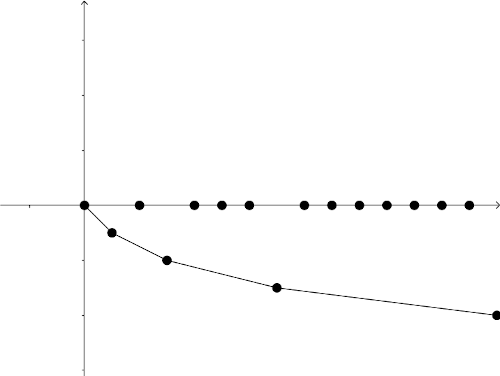
\includegraphics[scale=1.5]{/home/carlo/Tesi/images/figure_extra_2}
				\caption{Newton polygon of $f(X)$ for $p=2$}
				\label{figure:figure-extra-2}
			\end{figure}
		\end{example}
		Finally, we'll show a nice application of \cref{thm:weierstrass-padic-preparation}, which will imply the non-existence of a non-constant power series which converges on $\Cp$ and is never zero. This means exactly that we cannot have an exponential with the same properties of the classical one: in-fact in the classical case, if $h(X)$ is a convergent power series, then $e^{h(X)}$ is everywhere convergent and non-zero. We'll first need a technical lemma.
		\begin{lemma}
			\label{lemma:infinite-zeroes}
			Let $f(X)$ be a power series which converges on $D(p^{\lambda})$. If $f(X)$ has an infinite number of zeroes on $D(p^{\lambda})$ then $f(X)$ is identically zero.
		\end{lemma}
		\begin{proof}
			If $f(X) = 0$ there's nothing to prove, otherwise we can assume, by contradiction, $f(X) \in 1 + X\Cp\ser{X}$ (we can write $f(X) = a_dX^d \cdot g(X)$, where $d$ is such that $a_d$ is the first non-zero coefficient and study $g(X) \in 1 + X\Cp\ser{X}$). We can then apply \cref{thm:weierstrass-padic-preparation}, using $\lambda$, to obtain $N \in \N$, $h(X) \in 1 + X\Cp[X]$, a polynomial of degree $N$, and $g(X) \in 1 + X\Cp\ser{X}$, a power series convergent and non-zero on $D(p^{\lambda})$, such that
			\[
				h(X) = f(X) \cdot g(X).
			\]
			By hypothesis, $f(X)$ has infinite zeroes in $D(p^{\lambda})$ and, since $g(X)$ is never zero on $D(p^{\lambda})$, $h(X)$ must have infinite zeroes on $D(p^{\lambda})$. But $h(X)$ is a non-zero polynomial of degree $N$ so it cannot have infinite zeroes, and this is a contradiction. Thus the only possible case is $f(X) = 0$.
		\end{proof}
		\begin{prop}
			Let $f(X) = 1 + \sum_{i=1}^{+\infty} a_iX^i \in 1 + X\Cp\ser{X}$ be an everywhere convergent power series. For every $\lambda$, let $h_{\lambda}(X)$ be the polynomial obtained applying \cref{thm:weierstrass-padic-preparation}. Then $h_{\lambda} \to f$ as $\lambda \to +\infty$ (i.e., each coefficient of $h_{\lambda}$ converges to the corresponding coefficient of $f$). In particular, if $f$ is not a polynomial, then its zeroes are $(r_n)_{n \geq 1}$ (i.e. they're countable infinite) and 
			\[
				f(X) = \prod_{i=1}^{+\infty} \left(1 - \frac{X}{r_i}\right).
			\] 
		\end{prop}
		\begin{proof}
			If $f(X)$ is a polynomial, then the statement is trivial. From now on we'll consider $f(X)$ to be a proper power series. It's clear that such an $f$ must have a type $(1)$ Newton polygon. Let $(\lambda_n)_{n \geq 1}$ be the slopes of $\mathfrak{N}(f)$ (clearly we consider them in order, i.e. such that $\lambda_1 < \lambda_2 < \dots < \lambda_n < \dots$). Since $f(X)$ converges everywhere, by \cref{prop:newton-polygon-radius-convergence} we must have $\lim_{n \to +\infty} \lambda_n = +\infty$. It is also clear that $f$ has a countable infinite set of zeroes (there's clearly no contradiction here, because the zeroes are in $\Cp$): in-fact, applying \cref{corollary:newton-polygon-zeroes}, we obtain that for any segment of $\mathfrak{N}(f)$ we have a finite number of zeroes (and clearly the segments of the Newton polygon are countable infinite). Let it be $(r_n)_{n \geq 1}$, where they're listed in such a way that the first ``cluster'' corresponds to slope $\lambda_1$, the second to slope $\lambda_2$ and so on. Applying \cref{thm:weierstrass-padic-preparation} with $\lambda = \lambda_n$ we obtain a polynomial $1 + X\Cp[X] \ni h_n(X) := h_{\lambda_n}(X)$ and a power series $g_n(X) \in 1 + X\Cp\ser{X}$, convergent and non-zero on $D(p^{\lambda_n})$, such that
			\[
				h_n(X) = f(X) \cdot g_n(X).
			\]
			Let's introduce some terminology:
			\begin{gather*}
				h_n(X) = 1 + \sum_{i=1}^{d_n} a_{n,i}X^i, \qquad g_n(X) = 1 + \sum_{i=1}^{+\infty} b_{n, i}X^i,
			\end{gather*}
			where we set $d_n := \deg h_n(X)$. By \cref{thm:weierstrass-padic-preparation} we know that $d_n$ is the total horizontal length of segments of $\mathfrak{N}(f)$ with slope less or equal to $\lambda_n$ and this also means that
			\[
				h_n(X) = \prod_{j=1}^{d_n} \left(1 - \frac{X}{r_j}\right). \tag{$*$}
			\]
			First of all, let's prove that the sequences $(a_{n,m})_{n \geq 1}$ are all Cauchy \emph{uniformly} in $m$, i.e. we'll find an upper bound which doesn't depend on $m$. 
			Let $k \in \N$ be such that $\lambda_1 < \dots < \lambda_k < 0 \leq \lambda_{k+1}$, i.e. the first $k$ slopes of $\mathfrak{N}(f)$ are negative. Let's consider $r_1, \dots, r_{d_k}$, all the roots of $f$ (they're not necessarily distinct) corresponding to the negative slopes of $\mathfrak{N}(f)$. Then $\pabs{1/r_i} = p^{\ord r_i} > 1$, for every $1 \leq 1 \leq d_k$. Instead, for any other root $r_m$ with $m > d_k$ we have $\pabs{1/r_m} \leq 1$, since it corresponds to a non-negative slope. Let's set $M := \pabs{1/r_1}\cdots\pabs{1/r_{d_k}}$ (if all slopes are non-negative we simply set $M = 1$). Recalling the relations between coefficients and reciprocal of roots (using elementary symmetric polynomials), for $n \geq k$, by $(*)$, we have
			\[
				a_{n, m} = (-1)^m \cdot e_m\left(\frac{1}{r_1}, \dots, \frac{1}{r_{d_k}}, \frac{1}{r_{d_k + 1}}, \dots, \frac{1}{r_{d_n}}\right).
			\]
			Since for any $j > d_k$ we have $\pabs{1/r_j} \leq 1$, it's easy to see that
			\[
				\pabs{a_{n,m}} \leq \pabs{1/(r_1 \cdots r_{d_k})} = M,
			\]
			for any $m \in \N$ and $n \geq k$. We have found a common upper bound for all the coefficients of all the polynomials $h_n(X)$ with $n \geq k$. Now we have
			\[
				h_{n+1}(X) = h_n(X) \cdot \prod_{j=d_n+1}^{d_{n+1}} \left(1 - \frac{X}{r_j}\right)
			\]
			so we obtain
			\[
				a_{n+1, m} = a_{n, m} + \sum_{j=1}^m (-1)^j\cdot a_{n, m-j}\cdot e_j\left(\frac{1}{r_{d_n + 1}}, \dots, \frac{1}{r_{d_{n+1}}}\right),
			\]
			where we set $a_{n, 0} = 1$. Since $\lim_{n \to +\infty} d_n = +\infty$ (by construction) we can choose a large enough $n$ such that $\lambda_{n+1} > 0$. Then, $\pabs{1/r_j} = p^{\ord r_j} = p^{-\lambda_{n+1}} < 1$ for any $d_n + 1 \leq j \leq d_{n+1}$. Now it's easy to see that 
			\begin{gather*}
				\forall\, j \in \N, \quad  \pabs{e_j\left(\frac{1}{r_{d_n + 1}}, \dots, \frac{1}{r_{d_{n+1}}}\right)} \leq \pabs{\frac{1}{r_{d_n + 1}}} = p^{-\lambda_{n+1}} \\
				\implies \pabs{a_{n+1, m} - a_{n,m}} = \max_{1 \leq j \leq m} \pabs{a_{n, m-j}\cdot e_j\left(\frac{1}{r_{d_n + 1}}, \dots, \frac{1}{r_{d_{n+1}}}\right) } \leq M \cdot  p^{-\lambda_{n+1}}.
			\end{gather*}
			Since  $\lim_{n \to +\infty} p^{-\lambda_{n+1}} = 0$, $(a_{n, m})_{n \geq 1}$ is Cauchy (see \cref{lemma:cauchy-sequence-ultrametric}). Let's observe that our bounds don't depend on $m$, i.e. $\pabs{a_{n+1, m} - a_{n, m}} \leq M\cdot p^{-\lambda_{n+1}}$ for any $m \in \N$ and $n \geq k$. Since $(\lambda_n)_{n \geq 1}$ is non-decreasing, for $m > n \geq k$ we obtain
			\[
				\pabs{a_{m, i} - a_{n, i}} \leq \max_{n \leq j < m}\pabs{a_{j+1, i} - a_{j,i}} \leq \max_{n \leq j < m} Mp^{-\lambda_{j+1}} = Mp^{-\lambda_{n+1}}.
			\]
				
			Now, we know that $g_n(X)$ converges and is non-zero on $D(p^{\lambda_n})$; this means exactly that, if $\gamma_n$ is the first slope of $\mathfrak{N}(g_n)$, then $\gamma_n > \lambda_n$. In-fact, $\gamma_n \leq \lambda_n$ would imply, by \cref{corollary:newton-polygon-zeroes}, the existence of $\alpha \in \Cp$ such that $\pabs{\alpha} = p^{\gamma_n} \leq p^{\lambda_n}$ such that $g(\alpha) = 0$ and this cannot be the case. From a geometrical point of view, this means that every point $(i, \ord b_{n,i})$ lies on or above the line $y = \gamma_n \cdot x$, i.e.
			\[
				\ord b_{n,i} \geq i \cdot \gamma_n.
			\]
	 		We have already proved that $\lim_{n \to +\infty} \lambda_n = +\infty$ so $\lim_{n \to +\infty} \gamma_n = +\infty$ and this implies $\lim_{n \to +\infty} \ord b_{n,i} = +\infty$, i.e. $\lim_{n \to +\infty} b_{n,i} = 0$ for every $i \geq 1$. Let's now come back to the relation $h_n(X) = f(X)\cdot g_n(X)$ and let's consider the single coefficients; we obtain 
			\begin{align*}
				a_{n, 1} &= b_{n,1} + a_1; \\
				a_{n, 2} &= b_{n,2} + a_1b_{n,1} + a_2; \\
				\vdots \\
				a_{n, m} &= b_{n, m} + \sum_{j=1}^{m-1} a_jb_{n, m-j} + a_m.
			\end{align*}
			Then, for any $m \geq 1$, we have $\lim_{n \to +\infty} a_{n, m} = a_m$. Let's fix $x \in D(1)$ and $\epsilon > 0$ and consider
			\begin{gather*}
				\pabs{f(x) - h_n(x)} = \pabs{\sum_{i=1}^{+\infty} (a_i - a_{n, i}) x^i} \leq \max\left\{\max_{1 \leq i \leq d_n} \pabs{a_i - a_{n,i}},\, \max_{i > d_n}\,\pabs{a_i} \right\}
			\end{gather*}
			where we set $a_{n, i} = 0$ if $i > d_n$. We already know $\lim_{n \to +\infty} d_n =+\infty$ and we know that $\lim_{i \to +\infty} \pabs{a_i} = 0$ since $f$ converges everywhere (see \cref{prop:summable_families}). Let's choose $n \in \N$ such that $i > d_n$ implies $\pabs{a_i} < \epsilon$. Now we have only to give an upper bound on the first term, but this is easy thanks to the bounds we proved before:
			\begin{gather*}
				\pabs{a_i - a_{n, i}} = \lim_{m \to +\infty} \pabs{a_{m, i} - a_{n, i}} \leq \lim_{m \to +\infty} Mp^{-\lambda_{n+1}} = Mp^{-\lambda_{n+1}} \\
				\implies \max_{1 \leq i \leq d_n} \pabs{a_i - a_{n,i}} \leq M\cdot p^{-\lambda_{n+1}}
			\end{gather*}
			and we can assume that $n \in \N$ is big enough such that $M\cdot p^{-\lambda_{n+1}} < \epsilon$ and $i > d_n$ implies $\pabs{a_i} < \epsilon$. Since $\epsilon$ is chosen arbitrarily, we conclude that if $x \in D(1)$ then
			\[
				f(x) = \lim_{n \to +\infty} h_n(x) = \lim_{n \to +\infty} \prod_{j=1}^{d_n} \left(1 - \frac{x}{r_j}\right) = \prod_{j=1}^{+\infty} \left(1 - \frac{x}{r_j}\right).
			\]
			Let's define $\ell(X) := \prod_{j=1}^{+\infty} \left(1 - \frac{X}{r_j}\right)$. It can be proved that $\ell(X) \in 1 + X\Cp\ser{X}$ exploiting the fact that $\lim_{n \to +\infty} \pabs{1/r_n} = 0$ and that its coefficient of $X^m$ is simply the sum of the series of all possible products of $m$ of the $-1/r_i$'s (which converges). Now, $\ell(X)$ converges on $D(1)$ because $\ell(x) = f(x)$ for any $x \in D(1)$. We can conclude that, in $\Cp\ser{X}$, we have
			\[
				f(X) = \ell(X) = \prod_{j=1}^{+\infty} \left(1 - \frac{X}{r_j}\right) 
			\]
			since $g(X) := f(X) - \ell(X)$ is a power series convergent on $D(1)$ with infinite zeroes and, by \cref{lemma:infinite-zeroes}, it must be $g(X) = 0$. 	
		\end{proof}
		This proposition resembles a lot the Weierstrass factorization theorem of complex analysis, although the \padic result is much more clean: there are no exponential factor in the product. One immediate implication is that any power series which converges everywhere and is never zero must be a constant: here is why we cannot have an exponential similar to the classic one, which converges everywhere, is never zero but isn't constant. Finally we can think as power series which converges everywhere simply as ``polynomials with infinite zeroes'', which can be factorized in the same exact way we factorize polynomials. 
		
	\backmatter
	%\chapter{Basic Notations}
		\begin{itemize}
			\item $\R^+ = \R_{\geq 0} = [0, +\infty[$
			\item $\N = \{0, 1, 2, ...\}$ 
			\item WLOG = Without Loss Of Generality
			\item PID = Principal Ideal Domain
			\item $\delta_{i, j} = \delta_i^j$ is the Kronecker symbol (it's $1$ if $i=j$ and $0$ otherwise)
			\item If $(X, d)$ is a metric space, $B_{<r}(a) := \{x \in X \mid d(a, x) < r \}$ and $B_{\leq r}(a) := \{x \in X \mid d(a, x) \leq r \}$
			\item If $A$ is a set, $\#A = |A| = \text{card}(A)$
		\end{itemize}

	\chapter{\bibname}
	\nocite{robert:padic-analysis, koblitz:padic-numbers, bourbaki:topologie, chen:padics, michon:padic-arithmetic, thorne:teichmuller, conrad:algebraic-closure}
	%\printbibliography[heading=book, category=book]
	%\printbibliography[heading=online, category=online]
	\bibbycategory
\end{document} 